\documentclass[oneside, 12pt]{report}
\usepackage[utf8]{inputenc}
\usepackage{graphicx}
\graphicspath{ {./} }

\pagenumbering{arabic}

\usepackage{geometry}

\usepackage{setspace}
\onehalfspacing

\geometry{a4paper, margin=2.5cm}
\usepackage[pdflang={en-GB}]{hyperref}

\usepackage{amsmath}
\numberwithin{equation}{section}
 
\usepackage{float}

\usepackage{chemformula}
\usepackage{cleveref}
\usepackage{siunitx}
\DeclareSIUnit\angstrom{\text {Å}}

\usepackage{multirow}

\usepackage{booktabs}
\usepackage{tabulary}

\usepackage[font={small,it},labelfont=bf]{caption}
\usepackage{subcaption}

\usepackage[T1]{fontenc}

\usepackage{listings}

\usepackage{caption} %Adds captions to figures
\usepackage{subcaption}

%\usepackage[table]{xcolor} 
\usepackage{tabularx}%Inserts table

\usepackage[acronym]{glossaries}
\makeglossaries

\newacronym{ir}{IR}{Infrared}
\newacronym{em}{EM}{Electromagnetic}
\newacronym{thz}{THz}{Terahertz}
\newacronym{tds}{THz-TDS}{THz Time-Domain Spectroscopy}
\newacronym{tpi}{TPI}{Terahertz Pulsed Imaging}
\newacronym{dft}{DFT}{Density Functional Theory}
\newacronym{alm}{\(\alpha\)LM}{\(\alpha\)-Lactose Monohydrate}
\newacronym{xrd}{XRD}{X-Ray Diffraction}
\newacronym{vdos}{VDOS}{Vibrational Density of States}
\newacronym{pc}{PC}{Photoconductive}
\newacronym{eo}{EO}{Electro-Optic}
\newacronym{snr}{SNR}{Signal-to-Noise Ratio}
\newacronym{cw}{CW}{Continuous Wave}
\newacronym{bbo}{BBO}{\(\beta\)-Barium Borate}
\newacronym{qcl}{QCLs}{Quantum Cascade Lasers}
\newacronym{td}{TD}{Time Domain}
\newacronym{fd}{FD}{Frequency Domain}
\newacronym{si}{SI}{Semi-Insulating}
\newacronym{lt}{LT}{Low Temperature Grown}
\newacronym{ft}{FT}{Fourier Transform}
\newacronym{rms}{RMS}{Root Mean Squared}
\newacronym{hf}{HF}{Hartree-Fock}
\newacronym{mbse}{MBSE}{Many Body Shr\"{o}dinger Wavefunction}
\newacronym{lda}{LDA}{Local Density Approximation}
\newacronym{gga}{GGA}{Generalised Gradient Approximation}
\newacronym{bz}{BZ}{Brillouin Zone}
\newacronym{sto}{STO}{Slater Type Orbital}
\newacronym{gto}{GTO}{Gaussian Type Orbital}
\newacronym{dfpt}{DFPT}{Density Functional Perturbation Theory}
\newacronym{pbe}{PBE}{Perdew-Burke-Ernzerhof}
\newacronym{dc}{DiC}{Dispersion Correction}
\newacronym{ts}{TS}{Tkatchenko-Scheffler}
\newacronym{bj}{BJ}{Becke-Johnson}
\newacronym{paw}{PAW}{Projector Augmented-Wave}
\newacronym{ptfe}{PTFE}{Polytetrafluoroethane}
\newacronym{fwhm}{FWHM}{Full Width at Half Maxiumum}
\newacronym{vdw}{VDW}{Van der Waals}
\newacronym{ipa}{IPA}{Isopropyl Alcohol}
\newacronym{uv}{UV}{Ultraviolet}
\newacronym{atr}{ATR}{Attenuated Total Reflectance}
\newacronym{ftir}{FTIR}{Fourier-Transform Infrared Spectroscopy}
\newacronym{ho}{HO}{Harmonic Oscillator}
\newacronym{md}{MD}{Molecular Dynamics}
\newacronym{qha}{QHA}{Quasi-Harmonic Approximation}
\newacronym{tpx}{TPX}{Polymethylpentene}

\usepackage[style=ieee,sorting=none, citestyle=numeric-comp, backend=bibtex, url=false, doi=false, isbn=false, maxbibnames=99]{biblatex}
\addbibresource{references} %Adds bibliography

\pagenumbering{roman}
\begin{document}

\setlength{\parskip}{5pt}

\begin{titlepage}
   \begin{center}
       \vspace*{4cm}

       \huge \textbf{Investigation and Analysis of Phenomena in the Far-Infrared Region}\\
            
       \vspace{2cm}

       \large Calum Neil Alasdair Towler, MChem

       \vspace{4cm}
            
       \small \textit{Submitted in accordance with the requirements for the degree of Doctor of Philosophy}
            
       \vspace{1cm}
            
       \large \textbf{The University of Leeds}\\
       School of Chemistry\\

        \vspace{2cm}
       
       December 2022
            
   \end{center}
\end{titlepage}
% maybe find a style that groups columns to fixed size

\chapter*{Declaration}
The candidate confirms that the work submitted is his own, except where work which has formed part of jointly authored publications has been included. The contribution of the candidate and the other authors to this work has been explicitly indicated below. The candidate confirms that appropriate credit has been given within the thesis where reference has been made to the work of others.

Two publications have arisen from the work presented in this thesis, both from work detailed in Chapter~4:

\textbf{C. N. A. Towler}, J. Kendrick, and A. D. Burnett, “Understanding the effect of dispersion corrections on the calculated spectra of \(\alpha\)\nobreakdash-lactose monohydrate,” in \textit{2020 45th International Conference on Infrared, Millimeter, and Terahertz Waves (IRMMW\nobreakdash-THz)}, 2020, pp. 1\nobreakdash–2. 25

\vspace{0.1cm}

The time\nobreakdash-domain spectroscopy system used to measure the terahertz absorption spectrum at \SI{4}{K} was originally designed by Dr. Andrew Burnett. The software used to produce terahertz absorption spectra from calculated mode frequencies and intensities was written by Dr. John Kendrick. I collected all the data, produced all the figures and wrote the initial and final drafts of this paper, with all authors contributing between these drafts.

\vspace{0.7cm}

A. D. Burnett, \textbf{C. N. A. Towler}, and J. Kendrick, “Calculating the complex permittivity of powdered crystalline materials,” in \textit{2019 44th International Conference on Infrared, Millimeter, and Terahertz Waves (IRMMW\nobreakdash-THz)}, 2019, pp. 1–2. 9

\vspace{0.1cm}

I produced the data and designed the figure for the comparison of the calculated and experimental terahertz absorption spectra of \(\alpha\)\nobreakdash-Lactose Monohydrate. No other contribution to this work occurred.

This copy has been supplied on the understanding that it is copyright material and that no quotation from the thesis may be published without proper acknowledgement.

The right of Calum Neil Alasdair Towler to be identified as Author of this work has been asserted by Calum Neil Alasdair Towler in accordance with the Copyright, Designs and Patents Act 1988.



\clearpage
\vspace*{10cm}
\begin{center}
    {\textit{This thesis is dedicated to my wonderful parents}}
\end{center}


\chapter*{Acknowledgements}
Firstly, I want to extend my enormous gratitude to Dr. Andrew Burnett who was my primary supervisor throughout my PhD and my Masters project. His support, guidance and patience has been invaluable throughout and I will forever be thankful for everything. Not only did he provide vital knowledge and direction but he also assisted with motivation and perspective when, owing to various difficult challenges during the PhD, these were not substantial.

I would also like to extend my thanks to Dr. Aniela Dunn, Dr. Thomas Gill, Dr. Joshua Freeman and Dr. David Bacon, as well as the other members of the University of Leeds Terahertz Group, for providing their expertise and assistance when I was often out of my depth. From monitoring me in the clean room to endlessly diagnosing issues with the various experimental set-ups, their help was a critical element of my success in this project.

To my parents, and by extension my siblings and their children, your unwavering support over the last few years has made this project possible. Thank you so much for helping me attain this monumental achievement. 

Finally, to my friends old and new. Thank you all for the wonderful times over the last few years. In particular, I would like to thank my friends Sam and Emma, who were there for me at every step and who kept me happy and alive during those critical junctures. 

Thank you, again, everyone.


\chapter*{Abstract}
The far-infrared (IR) frequency range, or more specifically the terahertz (THz) frequency range, of the electromagnetic spectrum has been comparatively underutilised in the field of solid-state vibrational spectroscopy. This was historically owing to a lack of coherent sources and detectors but now stems from the challenges involved with the interpretation of the resultant spectra as the excited motions in this frequency range consist of complex motions that must be deciphered with the aid of computational simulation using methods such as Density Functional Theory (DFT). This, in turn, gives rise to its own challenges as the accurate simulation of large organic molecular crystals can be computationally expensive. 

In DFT, weak intermolecular bonds such as H-bonds are poorly represented and an empirical correction is often included to account for them. These are called dispersion corrections and an investigation into the appropriate dispersion correction for \(\alpha\)-Lactose Monohydrate (\(\alpha\)-LM) was conducted. This molecule was chosen owing to its uncommonly sharp absorption peaks in this frequency range. DFT uses the harmonic approximation to calculate vibrational mode frequencies but this will inevitably remove important anharmonic effects, such as thermal expansion, from the calculation which may reduce correlation between calculated and experimental spectra. The Quasi-Harmonic Approximation (QHA) allows for thermal expansion to be incorporated into the system by applying the harmonic approximation to a range of volumes. This was used to calculate the thermodynamic properties and temperature dependent mode properties of \(\alpha\)-LM. This in turn was used to calculate the THz absorption spectrum of \(\alpha\)-LM at \SI{300}{K}.

The primary source of THz radiation for broadband spectroscopy is photoconductive switches. These are excited with femtosecond laser pulses that are focused onto a gap between two electrodes. An investigation into the appropriate gap-size for a photoconductive switch being excited by a \SI{150}{mW} fibre laser was carried out, with the appropriate gap-size being determined to be \SI{20}{\micro\metre}.


\tableofcontents

\listoffigures
\listoftables

\printglossary[type=\acronymtype, nonumberlist, nopostdot]

\chapter{Introduction}
\pagenumbering{arabic}
\label{ch:int}
\input{Ch1_Introduction.tex}

\chapter{Generation and Detection of Terahertz Radiation and the Methodology of Terahertz Time-Domain Spectroscopy}
\label{ch:exp_theory}
There are now many methods of generating and detecting significant field strengths of coherent \acrshort{thz} radiation and these will be discussed in this chapter, with a particular focus on photoconductive (\acrshort{pc}) switches and electro\nobreakdash-optic (\acrshort{eo}) crystals. 
The custom\nobreakdash-built spectrometer and its variants that are used in this work will be described and the principle of \acrshort{tds} and the process of data collection will be explained. 
Finally, the method behind the extraction of spectral properties of measured samples and some of the challenges associated with this will be discussed.

\section{Terahertz Generation and Detection}
With the value of \(k_BT\) at room temperature being \SI{6.21}{\acrshort{thz}}, most matter emits \acrshort{thz} radiation but these emissions are weak, incoherent and not suitable for practical use. However, these weak emissions have been used in astronomy where spectral lines in the \acrshort{thz} region can be used for probing the composition and state of stellar objects~\cite{Stacey2011}.

Coherent \acrshort{thz} radiation sources can be broadly separated into two categories: electrical and photonic. Electrical sources generate \acrshort{thz} radiation through up\nobreakdash-conversion of lower\nobreakdash-frequency signals~\cite{Orihashi2005, Davies2002, Gold1998} or by utilising electron beams~\cite{He2013, Schmidt2002, Williams2002}, whereas photonic sources generate \acrshort{thz} radiation through down\nobreakdash-conversion of optical and \acrshort{ir} sources~\cite{McIntosh1995, Dai2011, Warren1991, Wu1995} or by direct THz emission~\cite{Williams2007,Faist1994} and are discussed in further detail below. Whilst no electrical sources are used in this work, there are a range of these sources that are used by the wider \acrshort{thz} community. 

One significant area of development in electronic \acrshort{thz} generation and detection has been in the area of \acrfull{qcl}, which can produce both continuous wave (\acrshort{cw}) \acrshort{thz} and pulsed \acrshort{thz} radiation in a narrow frequency region. In \acrshort{qcl}, sub\nobreakdash-bands are developed in a material through a variety of different methods~\cite{Williams2007}. Electronic transitions between these states can be manipulated to fall inside the \acrshort{thz} range. Quantum tunnelling allows a single electron to perform more than one of these transitions, producing the cascading effect after which the device is named~\cite{Faist1994}.
This frequency can often be tuned, with one group reporting a range of 2.06 – \SI{4.65}{\acrshort{thz}} with an output power of up to \SI{4.2}{\micro W}~\cite{Lu2016}. 
\acrshort{qcl} have been demonstrated to produce \SI{2.4}{W} in power in pulsed mode~\cite{Lin2017} and \SI{0.23}{W} in \acrshort{cw} mode~\cite{Wang2016}, and so a significant amount of research continues in the development of these devices for \acrshort{thz} generation. The high power available at selective frequencies may allow pumping of phonon modes for \acrshort{thz} pump spectroscopies. 
However, owing to the nature of these devices, the key limitation for this technology is the low temperatures required to operate it, resulting from the collapse of population inversion at higher temperatures~\cite{Williams2007}. The high powers demonstrated above were achieved at 10 and \SI{15}{K} respectively. This is problematic as techniques involving cryogens add to the complexity and cost of an overall procedure and these tend to be the main sources of temperature control. Therefore, another key area of development for \acrshort{qcl} has been in raising their operational temperatures. Currently, the highest operational temperature in pulsed mode is \SI{250}{K}~\cite{Khalatpour2020}, recently rising to \SI{261}{K}~\cite{Khalatpour2022}, and \SI{129}{K}~\cite{Biermann2014} for \acrshort{cw}, but these produce significantly less output power.
Recently, it was demonstrated that thermo\nobreakdash-electric cooling can replace cryogens for this purpose~\cite{Kainz2019}. This allows low temperatures to be reached using a simpler and cheaper method, increasing the accessibility of this technique.
Whilst simply operating \acrshort{qcl}, they only act as \acrshort{thz} generators but through self\nobreakdash-mixing~\cite{Keeley2017}, \acrshort{qcl} can act as detectors and a single device has been demonstrated as being able to act simultaneously as a generator and detector for the purposes of gas spectroscopy~\cite{Linfield2018}. \acrshort{qcl} can also be used as detectors when combined with electronic components such as Schottky diodes~\cite{Wanke2010}.
Some modern applications of \acrshort{qcl} are using these devices on satellites for the study of species in the Earth's upper atmosphere layers~\cite{Swinyard2016}, imaging~\cite{Dean2014} and wireless communication~\cite{Chen2011}. Whilst these devices show tremendous promise for the future of many \acrshort{thz} applications, the ability of \acrshort{qcl} to generate radiation below \SI{1}{\acrshort{thz}} is lowered as maintaining the required population inversion becomes much more difficult at lower frequencies. This has been achieved using strong magnetic fields~\cite{Wade2008} which complicates the system design significantly.

Solid\nobreakdash-state electrical devices capable of frequency\nobreakdash-multiplying lower\nobreakdash-frequency signals have been pursued owing to the comparatively significant development in microwave generation technology. However, these struggle to get to frequencies above \SI{1}{THz}~\cite{Kinev2021}. Devices like Schottky diodes which have been demonstrated to be capable of rapid sampling rates that enable real\nobreakdash-time observation of changes to systems such as wetting or protein unfolding~\cite{Rettich2015}.

The main alternative photonic sources are photomixers~\cite{McIntosh1995}, where high frequency optical femtosecond lasers are focused and combined onto a \acrshort{pc} switches to produce coherent \acrshort{cw} \acrshort{thz} radiation at a narrow frequency for applications surrounding non-linear optical effects. These devices have seen significant development using a range of materials to increase efficiency~\cite{AlMuhadar2022}.
It was demonstrated that by focusing an optical beam onto the ambient gases in air a plasma is formed that emits low frequency EM radiation~\cite{Hamster1993} and development in this area has resulted in a procedure where a \acrfull{bbo} crystal is used to generate the second harmonic of the incident beam. The combination of these is focused onto air which will ionise and emit a broadband THz pulse with a bandwidth of up to \SI{30}{THz}~\cite{Dai2011}. This technique allows coherent emission and detection throughout the \acrshort{ir} range which is a significant improvement on most current techniques. However, an amplified laser is required which typically utilise lower repetition rates in order to generate the high powers required. With lower repetition rates comes a reduction in data samples which will decrease the \acrshort{snr} on the extracted data.

\subsection{Photoconductive Switches}
\label{subsec:pcswitches}
For spectroscopic applications, photoconductive (\acrshort{pc}) switches~\cite{Warren1991} are widely used as a source of pulsed, coherent \acrshort{thz} generation and as a \acrshort{thz} detector. A \acrshort{pc} switch, shown in \Cref{fig:PCA}, consists of a semiconductor that is coated with a pair of Au electrodes, using a thin Ti layer as an adhesive to help the Au bind more cohesively. These electrodes are deposited in a way that leaves a small gap that where the size of the gap is on the order of tens to hundreds of microns. A femtosecond laser is focused onto this gap, where it generates electron\nobreakdash-hole pairs in the semiconductor if the laser energy is larger than or equal to the bandgap of the semiconductor. A bias is applied across the gold electrodes, which accelerates the charge carriers across the gap~\cite{Auston1984}. \acrshort{thz} radiation is generated without applying a bias through the photo\nobreakdash-Dember effect~\cite{Vaisakh2014} but significantly more photocurrent is generated in the semiconductor when a bias is applied. The bias is usually electrically chopped to allow for lock\nobreakdash-in detection. This acceleration produces a transient current in the surface of the semiconductor, radiating a single\nobreakdash-cycle coherent \acrshort{thz} wave~\cite{Burford2017} with an amplitude, \(E_{THz}\), proportional to the first derivative of the generated time dependent transient current \(J(t)\):

\begin{figure}
    \centering
    \includegraphics[width=0.4\textwidth]{Figures/Misc/Theory/PCA.png}
    \captionsetup{font = footnotesize, justification = centering}
    \caption[A Diagram of a Photoconductive Switch]{A diagram of a photoconductive switch. The gold electrodes are biased to accelerate charge carriers released upon absorption of an incident infrared pulse. These accelerating charge carriers radiate terahertz radiation in all directions which is collected using parabolic mirrors.}
    \label{fig:PCA}
\end{figure}

\begin{equation}
E_{THz} \propto{\frac{\delta J(t)}{\delta t}}
\end{equation}

This is proportional to both the incident optical fluence and the magnitude of the bias across the electrodes, which dictate the carrier density and velocity respectively. The generated photocurrent is defined as:

\begin{equation}
\frac{\delta J}{\delta t} = en\frac{\delta v}{\delta t} + ev\frac{\delta n}{\delta t}
\end{equation}

Where \(e\) is the carrier charge, \(v\) is the carrier velocity and \(n\) is the carrier density. This means that the waveform of the emitted \acrshort{thz} radiation depends on several factors including both the incident laser pulses and the characteristics of the material used for the semiconducting layer. As shown in \Cref{fig:exampletd}, the \acrshort{thz} signals measured in the time domain (\acrshort{td}) in this work consist of a large positive peak followed by a large negative peak and finishing with a series of oscillations. The laser pulsewidth and intensity control the magnitude of the positive peak, owing to the initial production and acceleration of charge carriers only occurring during illumination. The subsequent peak's magnitude and shape is related to the substrate composition, such as its resistivity, breakdown voltage and carrier lifetime. Having a high resistivity and breakdown voltage minimizes heating effects of dark current owing to the bias and allows for greater bias magnitudes, increasing the overall photocurrent generated across the gap~\cite{Warren1991, Tani1997_2}. This is important for increasing the maximum incident optical fluence or electrical bias across the \acrshort{pc} switch before the device breaks down. The width of the negative peak is dependent on the lifetime of the carriers, as shown in \Cref{fig:PCCarrierLifetime}. Controlling this parameter is important as the width of the peaks has a direct impact on the bandwidth available in the frequency domain (\acrshort{fd}).

\begin{figure}[t]
    \centering
    \includegraphics{Figures/Misc/Theory/PCsCarrierLifetime.png}
    \captionsetup{font = footnotesize, justification = centering}
    \caption[Calculated Photocurrent with Different Carrier Lifetimes]{Calculated photocurrent with different carrier lifetimes. Adapted from Winnerl \textit{et al.}~\cite{Winnerl2008}. Whilst the peak to peak magnitudes are similar for each pulse, their differing shape has an effect on the bandwidth in the frequency domain.}
    \label{fig:PCCarrierLifetime}
\end{figure}

\acrshort{pc} switches are limited in output owing to carrier screening, where the induced photocurrent generates its own electric field owing to the separation of charges, which interferes with the external electrical bias field. This results in saturation of the output \acrshort{thz} power, and increasing the incident optical fluence further can result in critical damage to the \acrshort{pc} switch~\cite{Kim2005} owing to heating and electrical breakdown. This is shown in \Cref{fig:saturation} where the flattening of the curve indicates that the \acrshort{pc} switch is close to breakdown and further increases in optical power will result in permanent damage and effective destruction of the \acrshort{pc} switch.

\begin{figure}
    \centering
    \includegraphics[scale=0.4]{Figures/Misc/Theory/OptSweepGaAs102G.png}
    \captionsetup{font = footnotesize, justification = centering}
    \caption[An Example of Saturation in a Photoconductive Switch]{An example of saturation in a photoconductive switch as optical power is increased. Further increases in the incident optical power would result in permanent damage to the device.}
    \label{fig:saturation}
\end{figure}

\begin{figure}
\begin{subfigure}{1\textwidth}
    \centering
    \includegraphics[scale=0.4]{Figures/Misc/SysDev/PKtoPKGvsSG.png}
    \caption{The peak to peak amplitudes of the sampled waveforms with increasing incident optical power for \SI{20}{\micro\metre} emitters.}
    \label{fig:sapphGaAspkpk}
    \vspace{10 mm}
\end{subfigure}
\vspace{10 mm}
\begin{subfigure}{1\textwidth}
    \centering
    \includegraphics[scale=0.4]{Figures/Misc/Theory/SIGaAsvsSapphG.png}
    \caption{The time dependent amplitudes for each emitters at their maximum incident optical power, which was 120 and \SI{130}{mW} for SI\nobreakdash-GaAs and sapphire respectively.}
    \label{fig:saphGaAsTD}
\end{subfigure}
\captionsetup{font = footnotesize, justification = centering}
\caption[The Peak to Peak Amplitudes of the Terahertz Waveforms and the Time-Domain Waveforms for each Emitters Maximum Power]{The peak to peak amplitudes of the \acrshort{thz} waveforms and the \acrshort{td} waveforms for each emitters maximum power. The emitters are on sapphire and \acrshort{si}-GaAs substrates and the gap size for each is \SI{20}{\micro\metre}. The smaller amplitude and lower tolerance for higher optical powers in the case of the  \acrshort{si}-GaAs substrate emitter is clear to see.}
\label{fig:gaasvssapph}
\end{figure}

These \acrshort{pc} switches can also be used in reverse as detectors which involves the same femtosecond optical source as for generation but with no external bias across the gap, as the incoming \acrshort{thz} field provides the field to accelerate the generated charge carriers. The induced photocurrent is proportional to the strength of the \acrshort{thz} electric field at a given time and by using a mechanical delay line, that alters the length of the optical pulse path, the field strength across the whole \acrshort{thz} waveform can be measured. This results in a high signal-to-noise (\acrshort{snr}) ratio owing to the coherent nature of the incoming \acrshort{thz}.

The semiconductor used in this work is \acrfull{lt}-GaAs, but many others have been used~\cite{Burford2017, Bacon2021, Murakumo2016, Dietz2013, Gu2002, Bertulis2006, Collier2016}. \acrshort{lt}\nobreakdash-GaAs has been used as it contains As clusters which act as trapping sites, significantly reducing carrier lifetimes~\cite{Segschneider1997}. These can be increased through annealing up to \SI{600}{\degreeCelsius}, which increases the size and frequency of these clusters~\cite{Gregory2003}. Winnerl \textit{et al.}~\cite{Winnerl2008} demonstrated that when using \acrshort{si}\nobreakdash-GaAs, which has a significantly longer carrier lifetime of several hundreds of picoseconds compared to \(\sim\)\SI{300}{\femto\second} in LT-GaAs, the second peak in the THz trace disappeared. This reduces the overall signal magnitude, resulting in a lower \acrshort{snr}.
Originally, the LT\nobreakdash-GaAs was grown onto a semi\nobreakdash-insulating (\acrshort{si}) GaAs substrate but this did not generate particularly high electric field strengths and was vulnerable to severe damage from over\nobreakdash-biasing~\cite{Bacon2017}. This is owing to the lower electrical resistivity of the \acrshort{si}-GaAs substrate which resulted in a higher dark current and overheating when large biases and optical fluences are used. Several replacements have been found, including quartz~\cite{Bacon2017}, one of the most successful being sapphire~\cite{Russell2013, Bacon2021}. This is demonstrated in \Cref{fig:gaasvssapph}, where the difference between substrates is clear. Sapphire has a much higher electrical resistivity, meaning that the switches are now less at risk of damage from higher voltages, and larger field strengths can be obtained. \acrshort{thz} losses are much less significant than in \acrshort{si}\nobreakdash-GaAs, and as it is transparent to \SI{800}{nm} light, “backside” illumination is now possible. This is where the optical beam travels through the sapphire to the LT\nobreakdash-GaAs, and the produced \acrshort{thz} radiation is collected with minimal losses through the substrate and is shown in \Cref{fig:backandfrontillumination}. This maximises bandwidth and \acrshort{snr} which, with increased field strength, are all desirable attributes for \acrshort{thz} spectroscopy~\cite{Bacon2017}.

\begin{figure}
\begin{subfigure}{0.49\textwidth}
    \centering
    \includegraphics[scale=1.5]{Figures/Misc/Theory/PCAFrontsideIllum.png}
    \caption{Front\nobreakdash-side illumination of a \acrshort{pc} switch.}
    \label{fig:fsillum}
\end{subfigure}
\begin{subfigure}{0.49\textwidth}
    \centering
    \includegraphics[scale=1.5]{Figures/Misc/Theory/PCABacksideIllum.png}
    \caption{Back\nobreakdash-side illumination of a \acrshort{pc} switch.}
    \label{fig:bsillum}
\end{subfigure}
\captionsetup{font = footnotesize, justification = centering}
\caption[Schematic showing Front and Back-Side Illumination of a Photoconductive Switch]{Schematic showing front and back-side illumination of a photoconductive switch.}
\label{fig:backandfrontillumination}
\end{figure}

The materials themselves are not the only controlling factor for the magnitude and maximum operating parameters of a \acrshort{pc} switch. Reducing the size of the electrode gap both increases the carrier generation efficiency~\cite{Tani2002}, resulting in a higher \acrshort{thz} signal, and decreases the breakdown voltage~\cite{Stone2004}, lowering the maximum operational fluence or applicable electrial bias. Thus, a compromise is required resulting in a typical gap size on the order of 10\nobreakdash--\SI{100}{\micro\metre}, but in some cases up to \SI{200}{\micro\metre}~\cite{Bacon2017}. 

\subsection{Electro-Optic Crystals}
Whilst \acrshort{pc} switches were the primary method of \acrshort{thz} generation and detection throughout this work, 
another method of generation and detection which was also utilised is to use an electro\nobreakdash-optic (\acrshort{eo}) crystal~\cite{Wu1995}, such as of ZnTe, as shown in \Cref{fig:EO_Detection}. This utilises a phenomenon called the Pockel’s effect~\cite{vanderValk} where an electric field induces a birefringence in the non\nobreakdash-linear crystal. This is when a material's refractive index is dependent on the propagation direction and polarisation of incoming light. This birefringance causes the incoming linearly polarised optical beam to become slightly elliptically polarised. The transmitted beam is then directed through a quarter\nobreakdash-wave \((\lambda/4)\) plate which is rotated so that if no THz radiation is incident on the non\nobreakdash-linear crystal, the beam transmitted through the \(\lambda/4\) plate would be circularly polarised. The beam is then finally split into orthogonal \(x\) and \(y\) components a using a Wollaston prism. As the beam when no \acrshort{thz} beam is present is circularly polarised these \(x\) and \(y\) components are equal and the difference signal between them is 0. When \acrshort{thz} radiation is incident on the non\nobreakdash-linear crystal this causes the transmitted beam to be elliptical and a difference is seen between the \(x\) and \(y\) components of the beam. This difference is directly proportional to the applied \acrshort{thz} electric field and by scanning the time delay between the \acrshort{thz} and laser probe beam the full electric field of the \acrshort{thz} pulse can be mapped. 

\begin{figure}[b]
    \centering
    \includegraphics[scale=0.9]{Figures/Misc/Theory/EODetection.png}
    \captionsetup{font = footnotesize, justification = centering}
    \caption[A Schematic showing the Process of Detection using an Electro-Optic Crystal]{A schematic showing the process of detection using an electro-optic crystal.}
    \label{fig:EO_Detection}
\end{figure}

The difference in intensity between the two orthogonal components is detected using a pair of balanced photodiodes which are connected to a lock\nobreakdash-in amplifier. The \acrshort{thz} electric field can be calculated from this using:

\begin{equation}
I_y - I_x = \frac{I_0 \omega L}{c} n_0^3 r_{41} E_{THz}
\end{equation}

Where \(I_y\) and \(I_x\) are the optical intensities on each diode, \(I_0\) represents the beam intensity with no \acrshort{thz} signal, \(\omega\) is the angular frequency and \(n_0\) is the refractive index of the crystal at \SI{800}{nm}. \(L\) is the length of the \acrshort{eo} crystal, \(r_{41}\) is the linear \acrshort{eo} coefficient, which is material dependent, and \(c\) is the speed of light in a vacuum. The principle can also be used in reverse to generate \acrshort{thz} radiation. Owing to the differing propagation speeds of different frequencies of light through a medium, the optical and \acrshort{thz} pulses will interfere destructively if overlapping over a particular distance. This distance is called the coherence length and is dependent on the relative refractive index at the optical and \acrshort{thz} frequencies. At higher frequencies the coherence length is shorter which results in a drop off in spectral bandwidth for thicker crystals. This can be counteracted by using thinner crystals but these are both harder to align and are more fragile. This results in a trade\nobreakdash-off between spectral bandwidth and ease\nobreakdash-of\nobreakdash-use of the device when using \acrshort{eo} crystals for broadband spectroscopic purposes and so these tend to be used for narrow-band applications~\cite{Watanabe2018}. They have been used in this work in \Cref{ch:sys_dev} as detectors.

\section{Terahertz Time-Domain Spectroscopy}
\subsection{Terahertz Time-Domain Spectroscopy Systems Used in this Work}
\label{subsec:tdssystems}
In this work, three \acrshort{tds} set\nobreakdash-ups have been used and whilst there are some variations between the generation, detection and data processing methods, only one was used for producing \acrshort{tds} spectra. This will be referred to as System~1 and will be described in the most detail and will be the example system used to describe \acrshort{tds} in general. System~2, which was used for testing \acrshort{pc} switches and the specifications for System~3, which is still under construction, will be described further in \Cref{ch:sys_dev}.

\begin{figure}[h]
\centering
\includegraphics[scale=0.6]{Figures/Systems/EE_BBTHzTDS_V7.png}
\captionsetup{font = footnotesize, justification = centering}
  \caption[Schematic of System~1 which was used for taking the Terahertz Absorption Spectra of \(\alpha\)-Lactose Monohydrate]{Schematic of System~1 which was used for taking the terahertz absorption spectra of \(\alpha\)-Lactose Monohydrate.}
  \label{fig:BBTDS System}
\end{figure}

System~1 is shown in \Cref{fig:BBTDS System} and can be considered a typical \acrshort{tds} set\nobreakdash-up. The optical \SI{800}{nm} pulses are provided by a mode-locked Ti:sapphire laser (Vitara, Coherent) that produces repeating \SI{20}{fs} pulses, centred at \SI{800}{nm}, with a repetition rate of \SI{80}{MHz}. This main pulse train was focused onto a \acrshort{lt}\nobreakdash-GaAs \acrshort{pc} switch with a \SI{5}{mm} thick quartz substrate and a gap size of \SI{100}{\micro\metre}. This was biased at \SI{350}{V} with a \SI{7}{kHz} modulation frequency using a 50\% duty cycle for lock-in detection. After the emitted \acrshort{thz} radiation was collected, collimated and focused through the sample, it was recollected and focused onto another \acrshort{pc} switch with the same parameters as the emitting \acrshort{pc} switch. The induced current in the detecting \acrshort{pc} switch was amplified using a gain of \SI{20}{\unit{\nA.\V^{-1}}}. The time constant for the sampling rate was typically \SI{1}{ms} and the sensitivity of the lock\nobreakdash-in was typically set to \SI{0.01}{V}. The spectrum was constructed from the average of 60 scans with a frequency resolution of \SI{0.01}{\acrshort{thz}}. Owing to the thickness of the emitter there were no system reflections in the selected scan range. This is owing to the primary reflection coming from the substrate containing the emitter and when this substrate is thick enough, this reflection occurs far away enough in time so as not to obscure any temporal features of the \acrshort{thz} pulse. The sample and \acrshort{thz} beams were kept under a dry nitrogen atmosphere. Low temperature measurements were performed by mounting the sample pellet onto a coldfinger of a continuous\nobreakdash-flow helium cryostat (MicrostatHe, Oxford Instruments) which has a pair of polymethylpentene (\acrshort{tpx}) windows.

\subsection{Sample Preparation}
All samples were purchased as powders rather than single crystals and were mixed, usually with a low mass ratio, with \acrfull{ptfe}. This was compressed into a pellet with an approximate thickness of \SI{500}{\micro\metre} using a mass of \SI{10}{\tonne}, which is a force of approximately \SI{98000}{N}. The true thickness of the pellet \textit{in situ} is determined from the THz spectral measurement and this will be discussed in \Cref{subsubsec:thickness}. This process is done owing to the significant absorption of \acrshort{thz} radiation of a wide range of materials which reduces the effective bandwidth of the spectrum. By diluting the samples in a material such as \acrshort{ptfe}, which is very weakly\nobreakdash-absorbing in the \acrshort{thz} region, the effective bandwidth of the system can be extended. 

\subsection{Challenges of Terahertz Time-Domain Spectroscopy}
Owing to the nature of this detection technique, for a given position of the mechanical delay line, a discrete value of the \acrshort{thz} waveform is sampled. By varying the length of the pump beam with respect to the probe beam, which alters the arrival time of the optical pulses, the entire waveform can be sampled. The reverse set-up, where the delay line is active on the probe beam is also possible. In this work, the delay line moves at a constant velocity and samples periodically for a given time constant. Owing to errors produced through sampling while the stage is moving at a constant velocity,  a data\nobreakdash-set that is not constantly separated in time is produced and so these values are interpolated to give a set of values that are. As multiple scans of both the reference and the sample are taken, these are averaged in the \acrshort{td}. This improves \acrshort{snr} ratio by reducing noise with this effect increasing asymptotically with respect to the number of scans~\cite{Popescu1996}. For most systems considered in this work, 60 scans has been selected as the optimum compromise between \acrshort{snr} and measurement time.
The collected waveform is constructed by assuming that each emitted \acrshort{thz} waveform is identical between the incident optical pulses on the emitter and that conditions are constant throughout the measurement. This assumption will not remain true if factors like laser power or humidity are not kept constant but owing to the set-up used these factors are able to be controlled or accounted for. Humidity is monitored by a hygrometer and measurements are performed at < 1\% humidity, utilising a purge box pumped with dry air or nitrogen. The Ti:sapphire crystal is temperature-controlled to minimise the effects of heating on the output and is left to stabilise for at least an hour after being switched on before any measurements are taken. 
As \acrshort{thz} signals can vary over several orders of magnitude in amplitude, measures must be taken to improve \acrshort{snr}. A widely utilised method is using a lock\nobreakdash-in amplifier, which requires a reference frequency. The electrical bias applied to the emitter is electrically chopped using a square wave resulting in both the propagating wave and the detector output being modulated at the chopping frequency, which is widely utilised method of amplifying signals.

\section{Extraction of Spectroscopic Parameters}
Originally, the earliest function a \acrshort{thz} transmission system could perform was detection of water vapour~\cite{vanExt1989}, owing to strong absorptions at these frequencies. This then progressed to using traditional methods such as the Beer\nobreakdash-Lambert Law~\cite{Kasap2006} where the absorption of the sample is related to its concentration. This section details how to extract the desired spectroscopic parameters from the sampled electric field. An overview is depicted in \Cref{fig:dataextraction}. 

The process about to be summarised was developed and described in significant detail by Greenall~\cite{Greenall2017}. The first step is to average and window the \acrshort{td} data, upon which a discrete \acrfull{ft} is performed. The sample data is divided by the reference data to calculate the transfer function, \(H\). The transfer function is a quantitative representation of the spectroscopic system. The phase component of \(H\), \(\angle H\), is used to calculate the real refractive index which in turn allows the calculation of the magnitude of the transfer function, \(|H|\). Finally, this is used to calculate the absorption coefficient using the method described below~\cite{Greenall2017}.

\begin{figure}[b]
    \centering
    \includegraphics{Figures/Misc/Theory/SignalToParamFlow.png}
    \captionsetup{font = footnotesize, justification = centering}
    \caption[An Overview of the Data Extraction Process]{An overview of the data extraction process. Time-dependent electric time stamps can be used to calculate the refractive index and then the absorption.}
    \label{fig:dataextraction}
\end{figure}

\subsection{Relationship Between Spectroscopic Parameters}
The refractive index of a sample, \(n\), is the ratio between the phase propagation velocity in the medium and in a vacuum. As frequency is held fixed, this results in changes to the wavelength of the incident wave. When a wave propagates through a sample, some of the energy of the wave is absorbed and the wave is attenuated. The degree of attenuation is described by the frequency dependent extinction coefficient, \(\kappa\), which is related to \(n\) by:

\begin{equation}
\Tilde{n} = n - i\kappa
\end{equation}

Where \(\Tilde{n}\) is the complex, frequency dependent refractive index. \(\kappa\) describes the attenuation of the amplitude per unit length, but is used less frequently in a chemical setting than \(\alpha\), which is the absorption coefficient and is related to \(\kappa\) by:

\begin{equation}
\alpha = \kappa \frac{2\omega}{c}
\label{eqn:abs}
\end{equation}

Where \(\omega\) is the angular frequency and \(c\) is the speed of light in a vacuum. A dielectric can generally be modelled as an array of charges bound in various ways to a structure. For 
example, in an ionic crystalline material, positive and negative ions are arranged in a fixed structure which repeats in 3D. In molecular crystals, the ions are held together with chemical bonds. When an electric field is applied to the dielectric, these charges interact with the field and will displace from their original position, straining the inter and intra\nobreakdash-molecular forces that hold the crystal together. If this phenomenon occurs over a significant enough portion of the material, an electric dipole is induced which is proportional to the charge magnitude and displacement. This polarisation is proportional to the permittivity of the sample:

\begin{equation}
P = (\Tilde{\epsilon}-1) \epsilon_0 E
\end{equation}

Where \(P\) is the induced polarisation, \(\Tilde{\epsilon}\) is the complex permittivity, \(\epsilon_0\) is the permittivity of free space and \(E\) is the incident electric field. This relationship arises from the coupling of the electric wave to the polarisation of the dielectric, which impedes the wave~\cite{Kasap2006}. Therefore, the complex permittivity is equal to the square of the complex refractive index and so the refractive index is dictated by the polarisation mechanisms in the sample.  The relationship between refractive index and permittivity can be expanded to:

\begin{equation}
\Tilde{\epsilon} = \Tilde{n}^2 = (n - i\kappa)^2
\end{equation}

The complex permittivity can be split into real and imaginary parts too:

\begin{equation}
\Tilde{\epsilon} = (\epsilon' - i\epsilon'') = (n^2 - \kappa^2) - i(2n\kappa)
\end{equation}

Where \(\epsilon'\) is the real permittivity and represents the ratio between the capacitance of a vacuum and of a dielectric. \(\epsilon''\) is the complex permittivity and describes the energy lost in coupling between the electric field and the dielectric polarisation. Substituting in using \Cref{eqn:abs}, this expression now demonstrates the relationship between permittivity and absorption:

\begin{equation}
\Tilde{\epsilon} = \left(n^2 - \frac{\alpha c^2}{2\omega}\right) - i\left(n\frac{\alpha c}{\omega}\right)
\end{equation}

\subsection{Transfer Model}
To extract these parameters from the collected data, a model relating them to the transfer function of the system has been developed~\cite{Duvillaret1996}. 

\begin{figure}
\centering
\begin{subfigure}{0.49\textwidth}
    \centering
    \includegraphics[scale=0.6]{Figures/Misc/Theory/TransferModel_Basic.png}
    \captionsetup{font = footnotesize, justification = centering}
    \caption{A model of a \acrshort{thz} pulse interacting with a sample’s surface. Most of the pulse is transmitted but a small amount is reflected.}
    \label{fig:transfermodel1}
\end{subfigure}
\begin{subfigure}{0.49\textwidth}
    \centering
    \includegraphics[scale=0.6]{Figures/Misc/Theory/WaveAttenuation.png}
    \captionsetup{font = footnotesize, justification = centering}
    \caption{The effect of propagation through a sample on a \acrshort{thz} wave (depicted as a sine wave for clarity). The wavelength decreases as the wave velocity decreases and the wave is attenuated.}
    \label{fig:waveattentuation}
\end{subfigure}
\captionsetup{font = footnotesize, justification = centering}
\caption[Extraction of Experimental Peak Widths]{The process of extracting peak properties from the experimental terahertz absorption spectrum.}
\label{Fig:transfermodel}
\end{figure}

When a \acrshort{thz} wave reaches an interface, such as the sample’s edge, a fraction of the \acrshort{thz} radiation is reflected whilst the rest propagates through, as shown in \Cref{fig:transfermodel1}. The ratio between these components is the transmission coefficient, \(T_{1,2}\), and is dictated by the relative refractive indices of the two mediums, \(\Tilde{n}_1\) and \(\Tilde{n}_2\). This is calculated by:

\begin{equation}
T_{1,2} = \frac{2\Tilde{n}_2}{\Tilde{n}_1 + \Tilde{n}_2}
\end{equation}

The transmitted \acrshort{thz} radiation will then propagate through the material. In most suitable materials, the \acrshort{thz} radiation will be attenuated and will undergo a phase shift. This can be seen in \Cref{fig:waveattentuation}, where the incident wave has a greater amplitude and wavelength than the final wave. The ratio between the final and incident \acrshort{thz} waves, which is often complex, is the propagation coefficient of the sample, \(P_s\). This is thickness dependent, (where \(l\) is thickness), and is calculated by:

\begin{equation}
P_s = e^{-i\frac{\omega l}{c} \Tilde{n}}
\end{equation}

As both a sample and reference scan are required, a reference model is also required. An identical \acrshort{thz} wave propagates through dry air which will be displaced by the sample. The propagation coefficient, \(P_A\), is identical to \(P_S\) except that \(\Tilde{n} = 1\). These equations combine to provide a sample model:

\begin{equation}
E_{sam} = T_{A,S} P_S T_{S,A} E_0 H_{sys}
\end{equation}

Where \(T_{A,S}\) and \(T_{S,A}\) are the air-sample and sample-air transmission coefficients respectively, \(E_0\) is the incident \acrshort{thz} radiation and \(H_{sys}\) is the instrument transfer function. A similar model can be produced for the reference:

\begin{equation}
E_{ref} = P_A E_0 H_{sys}
\end{equation}

\(E_0\) and \(H_{sys}\) are constant over both sample and reference measurements, and so when combined these should cancel out. In practice, this is not the case and this will be discussed further below when discussing reflections. By normalising the sample against the reference, the model transfer function, without considering reflections within the sample, will be:

\begin{equation}
H = \frac{E_{sam}}{E_{ref}} = T_{A,S} \frac{P_S}{P_A} T_{S,A} = \frac{4\Tilde{n}}{(\Tilde{n} + 1)^2} e^{-i\frac{\omega l}{c} (\Tilde{n}-1)}
\end{equation}

\subsection{Extraction of Refractive Index and Absorption}
By using simple assumptions which are valid whilst resonance does not occur in the sample, it is possible to derive expressions for the refractive index, \(n\) and extinction coefficient, \(\kappa\), individually.  In most relevant cases it can be assumed that the phase change over the measurement primarily occurs during propagation. This permits an expression in which the phase of the model transfer function can be equated to solely the propagation terms:

\begin{equation}
\angle H = \angle \frac{P_S}{P_A} = -\frac{\omega l}{c}(n-1)
\end{equation}

From this, \(n\) can be approximated as real and is calculated, and an expression for \(|H|\) can be formed:

\begin{equation}
|H| = \frac{4n}{(n+1)^2}e^{-\frac{\omega l}{c}\kappa}
\end{equation}

This is inverted to form an expression in terms of \(\kappa\), from which \(\alpha\) can be calculated using \Cref{eqn:abs}:

\begin{equation}
\kappa = \frac{-c}{\omega l} ln\left(|H|\frac{(n+1)^2}{4n}\right)
\end{equation}

\subsection{Dynamic Range}
As with all spectroscopic systems, there is an operating frequency range where signals below or above will not be detected. In addition to this, at frequencies close to the ends of this range, the detector noise will obscure signals owing to their low relative amplitude. This culminates in a noise floor, where detector noise completely obscures any measured signal. By normalising a reference measurement against the \acrfull{rms} of the noise floor, referred to as the dynamic range of the system, the frequency\nobreakdash-dependent maximum absorption, \(\alpha_{max}\), of the system for a specific sample can be determined. This means that signals less than this maximum absorption can be considered to be accurate, but any that are greater will be distorted by detector noise, providing an effective bandwidth for the system. This is shown in \Cref{fig:my_absconeat}.

\begin{figure}
    \centering
    \includegraphics[width=0.8\textwidth]{Figures/Spectra/AbsCoGNeat.png}
    \captionsetup{font = footnotesize, justification = centering}
    \caption[The Absorption Spectrum of \(\alpha\)-Lactose Monohydrate with the corresponding Maximum Absorption of the System]{The absorption spectrum of \(\alpha\)-Lactose Monohydrate with the corresponding maximum absorption of the system. The oscillations in the base absorption of the spectrum are called etalons. These are a consequence of reflections and will be discussed in \Cref{subsec:Reflections}.}
    \label{fig:my_absconeat}
\end{figure}

\subsection{Sample Reflections}
\label{subsec:Reflections}
Until this point, the model assumes that there is a single reflection that propagates in the reverse of the incident direction and does not reach the detector. This assumption can be correct if a time window is used to truncate out reflections, which can be done for thick, weakly absorbing samples. However, for a significant proportion of samples measured the first reflection can be present close enough to the main pulse that truncating them would result in either loss of frequency resolution or spectral information about the low frequency modes of the system. So spectral information is not lost, the model described above must be expanded to include these sample reflections.

If the reflection or reflections do not overlap with the oscillations from the main pulse, a window function is used to truncate the data so as to discard the reflection.  In this work, a Tukey window is used which is a rectangular window function but with a cosine roll-off.

\begin{figure}
    \centering
    \includegraphics{Figures/Misc/Theory/Window.png}
    \captionsetup{font = footnotesize, justification = centering}
    \caption[A Graph depicting a Tukey Window and its Effect on the Time-Domain Data]{A graph depicting a Tukey window and its effect on the time-domain data.}
    \label{fig:window}
\end{figure}

As shown in \Cref{fig:window}, the window function allows removal of reflections whilst maximising frequency resolution. If the reflections are not removed, they produce artefacts in the measured parameters called etalons, which can be seen in \Cref{fig:my_absconeat}. As the reflection is localised in time, this results in a sinusoidal error term in the extracted refractive index that is dependent on frequency~\cite{Greenall2017}. This propagates through to the rest of the spectral parameters as they are calculated from the refractive index.
The reflections can arise both from the sample or the system itself, from the emitter, detector or other optics in the beam path as each interaction with a material-air interface will cause a reflection.

\subsubsection{Incorporating Reflections into Model}
\begin{figure}
    \centering
    \includegraphics{Figures/Misc/Theory/TransferModel_Resonance.png}
    \captionsetup{font = footnotesize, justification = centering}
    \caption[The Sample Model updated to include Reflections]{The sample model updated to include reflections. Each time a sample-air interface is reached, a reflection occurs. The incident path has been offset for clarity but should be imagined as travelling perpendicular to the sample’s surface.}
    \label{fig:transferreflections}
\end{figure}

The assumptions about the sample and the beam are still held true, except that there is now a reflection each time the pulse reaches a sample-air interface. This creates a resonance within the sample, as shown in \Cref{fig:transferreflections}, where the beam has been directed at an angle for clarity. In reality, the beam is travelling perpendicular to the sample’s surface, as before. Each transmitted pulse appears as a delayed, attenuated copy of the original pulse, and their separation depends on the thickness and refractive index of the sample. The reflection coefficient of the system must now be considered, and is described by:

\begin{equation}
R_{1,2} = 1 - T_{1,2} = \frac{\Tilde{n}_2-\Tilde{n}_1}{\Tilde{n}_2+\Tilde{n}_1}
\end{equation}

This can be incorporated into expression for the model derived above, producing:

\begin{equation}
H = T_{A,S} \frac{P_S}{P_A} T_{S,A} (1+R_{S,A}^2 P_S^2)
\end{equation}

Which represents the original pulse transmitting entirely through the sample and an additional pulse that has reflected off the sample-air interface and propagated through the sample twice. Adding more reflections to the model is done by multiplying by \((1+R_{S,A}^2 P_S^2)\) for however many reflections are being considered. Whilst this model reduces etalons in the extracted parameters, they are not completely removed owing to uncertainty in the thickness measurement, and the degree of reduction is proportional to frequency. 

\subsubsection{Thickness Extraction}
\label{subsubsec:thickness}
\begin{figure}{t} 
\centering

\begin{subfigure}{0.49\textwidth}
\centering
\includegraphics[width=\textwidth]{Figures/Misc/Theory/ThicknessEffectonN.png}
\caption{Various refractive index values at different frequencies for different simulated thicknesses.}
\label{fig:thicknesseffect}
\end{subfigure}
\begin{subfigure}{0.49\textwidth}
\centering
\includegraphics[width=\textwidth]{Figures/Misc/Theory/ThicknessExtraction.png}
\caption{The Total Variance plotted against Thickness.}
\label{fig:thicknessextraction}
\end{subfigure}

\captionsetup{font = footnotesize, justification = centering}
\caption[The Effect of Different Thicknesses on the Refractive Index Values and the Thickness Extraction Curve]{The effect of different thicknesses on the refractive index values and the thickness extraction curve. In (a), a wide range has been plotted for clarity. In practice, a much smaller range of thicknesses is considered as shown in (b). The minimum corresponds to the thickness of the pellet.}
\label{Fig:thickness}
\end{figure}

An additional feature of this model is that it can be used to iteratively extract the thickness of the sample itself. This is critical in circumstances where a direct measurement of the sample is not possible, such as cryogenic experiments. A starting thickness is either assumed or measured and the steps detailed above are carried out. A range of sensible thicknesses are selected and the steps above are iterated through for each thickness. This produces a range of refractive index datasets, most of which will contain significant spectral artefacts.

By trying to minimise the total variance of the spectrum of the real refractive index, the optimal thickness can be selected. This corresponds to the smoothest trace in \Cref{fig:thicknesseffect}, but not all etalons can be removed this way. This method is used in \Cref{ch:ivdw} to extract the temperature\nobreakdash-dependent thickness of a pellet of \acrshort{alm}.

\section{Conclusion}
This chapter has described a variety of \acrshort{thz} generation and detection methods, focusing specifically on \acrshort{pc} switches and \acrshort{eo} crystals. Additionally, the process behind and the main system used for \acrshort{tds} in this work was described, as was the process of extraction spectroscopic parameters and some of the challenges behind this. 


\chapter{Density Functional Theory and its Applications for Vibrational Spectroscopy}
\label{ch:dft_theory}
\section{Introduction}
Owing to the complicated and varied nature of phenomena in the \acrshort{thz} range, interpretation of the measured spectral properties requires calculation of the nature, frequency and intensity of the underlying modes. These, in turn, are calculated from the electronic ground state of the system. This is achieved by solving the many-body Schr\"{o}dinger equation (\acrshort{mbse}), which is shown in \Cref{eqn:MBSE}, and in this work this will be achieved using \acrfull{dft} \cite{Kohn1965}.

\begin{equation}
\left( -\frac{1}{2}\sum_i\boldsymbol{\Delta}_i + \sum_i \boldsymbol{V}(\mathbf{r}_i) + \sum_{i\neq j}\frac{1}{ \lvert \mathbf{r}_i - \mathbf{r}_j \rvert } \right) \boldsymbol{\Psi} (\mathbf{r}_1, ..., \mathbf{r}_N) = \boldsymbol{E}\boldsymbol{\Psi} (\mathbf{r}_1, ..., \mathbf{r}_N)
\label{eqn:MBSE}
\end{equation}

\(\boldsymbol{\Delta}_i\) is the Laplace Operator acting on atom \(i\), \(\boldsymbol{V}(\mathbf{r}_i)\) is the potential energy, \(\mathbf{r}_i\) is the nuclear coordinates, \(\boldsymbol{\Psi}\) is the wavefunction and \(\boldsymbol{E}\) is the energy of the system. Initially, \acrshort{dft} was only used for very simple and uniform systems such as metals but development over the last few decades has enabled its use in for more complicated systems and studying chemical phenomena, such as pharmaceutically relevant compounds \cite{Berzins2020}, phase transformations in crystal structures \cite{Ruggiero2018, Paul2019}, nanomaterial properties \cite{Makkar2021} and amino acids \cite{Hachtel2019}. Other methods have been developed for attempting this and are widely used in the context of an isolated molecule in the gas phase. Whilst they can be used for periodic systems, they either tend to not match experimental data or become extremely expensive computations that can be unfeasible for large systems.

This chapter will describe \acrshort{dft} and the methodology of applying it to useful chemical systems, followed by a description of the software packages, general procedure and calculation parameters used. 

\section{Density Functional Theory}
\label{sec:DFTheory}
\subsection{Solving the Many Body Schr\"{o}dinger Equation}
Underpinning most quantum mechanical theories, \acrshort{dft} also uses the Born\nobreakdash-Oppenheimer approximation which states that any motion of a nucleus is much slower than the motion of an electron. This allows for an instantaneous response by the electron to the nucleus and as such, nuclei are treated as fixed in space, reducing the number of contributions to the total energy of the system. Attempting to solve the \acrshort{mbse} is too complex for all but the smallest systems so a number of simplifications have been developed over the years. In particular, the electron orbitals are defined to be one-electron non-interacting orbitals where:

\begin{equation}
\boldsymbol{\Psi} (\mathbf{r}_1, ..., \mathbf{r}_N) \xrightarrow{} \{\psi_1(\mathbf{r}),  \psi_2(\mathbf{r}), ..., \psi_N(\mathbf{r})\}
\end{equation}

\begin{equation}
\boldsymbol{\Psi}(\mathbf{r}_1, ..., \mathbf{r}_N) = \prod_i^N \psi_i (\mathbf{r}_i)
\end{equation}

These assumptions allow the separation of the total energy of the system, \(\boldsymbol{E}_{tot}\), into the following terms:

\begin{equation}
\boldsymbol{E}_{tot} = \boldsymbol{E}_{KE} + \boldsymbol{E}_{H} + \boldsymbol{E}_{Z} + \boldsymbol{U}_{Z} + \boldsymbol{E}_{XC} 
\label{eqn:GSComponents}
\end{equation}

where \(\boldsymbol{E}_{KE}\) is the kinetic energy of the electrons, \(\boldsymbol{E}_{H}\) is the Hartee energy which is the Coulombic potential energy, \(\boldsymbol{E}_{Z}\) is the potential energy between the electrons and the nuclei, \(\boldsymbol{U}_{Z}\) is the potential energy between the nuclei and \(\boldsymbol{E}_{XC}\) is the correlation exchange energy between the electrons. As these electron orbitals are non-interacting, each one has its own associated coordinate system in three dimensions. This results in a calculation that increases in magnitude as more electrons were added, which meant that calculations involving large amounts of electrons slowed down dramatically. Kohn, Honenburg and Sham \cite{Kohn1965, Hohenberg1964} developed a method that attempted to solve this. By defining each term in \Cref{eqn:GSComponents} as a functional dependent on the electron density, \(\rho\), the number of coordinates that needed to be calculated was reduced from \(3N\) to three. The total energy of the system can now be represented as:

\begin{equation}
\boldsymbol{E}[\rho] = \boldsymbol{E}_{KE}[\{\psi_i[\rho]\}] + \boldsymbol{E}_{H}[\rho] + \boldsymbol{E}_{Z}[\rho] + \boldsymbol{U}_{Z}[\rho] + \boldsymbol{E}_{XC}[\rho]
\end{equation}

The electron density is calculated using one electron orbitals, represented using basis sets, which are shown by:

\begin{equation}
\boldsymbol{\rho}(\mathbf{r}) = \sum_{i}^{\boldsymbol{N}} \lvert {\psi_i(\mathbf{r})} \rvert ^2
\end{equation}

This allows orbitals to be calculated as a linear combinations of atomic orbitals and this is discussed further in \Cref{subsec:bloch} and \Cref{subsec:pseudopot}. The Kohn\nobreakdash-Sham equation, which is a modified \acrshort{mbse}, is used to calculate these one electron orbitals with:

\begin{equation}
\left( -\frac{1}{2}\boldsymbol{\Delta} + V_z(\mathbf{r}) + V_H[\rho](\mathbf{r}) + V_{XC}[\rho](\mathbf{r)}\right) \psi_i(\mathbf{r}) =  \epsilon_i \psi_i (\mathbf{r})
\end{equation}

Each term can be calculated exactly with the exception of the final term, \(V_{XC}[\rho]\). This is the exchange correlation energy and represents the interaction between the electrons. These are described as functionals and there are many possible approximations for this, the simplest being the \acrfull{lda} \cite{Sahni1988}. This is where the electron density is assumed to be homogeneous. More complex functionals incorporate the gradient of the electron density as well and the simplest of these is called the \acrfull{gga} \cite{Perdew1996}. These can often be broken into separate exchange and correlation components that can be mixed to form new functionals such as meta\nobreakdash-\acrshort{gga}s \cite{Furness2021} and hybrid functionals such as B3LYP \cite{Stephens1994}. B3LYP is often used by the chemical community for small molecules but is computationally expensive. In this work, a version of \acrshort{gga} developed by Perdew \textit{et. al.} \cite{Perdew1996_2} has been used throughout this work and is referred to as the \acrfull{pbe} functional. This is a relatively simple functional that this group has previously shown can provide accurate results and is computationally efficient when compared to hybrid and meta functionals.

\subsection{Periodic Systems}
\label{subsec:bloch}
Whilst simplifying the \acrshort{mbse} drastically decreases the magnitude of the calculation, for crystals and other extended systems further simplification is needed as the number of electrons is still on the order of approximately \(10^{23}\). This is done by considering that the unit cell, the smallest infinitely repeating section of the crystal, must have the same orbitals at the same position in the unit cell regardless of where that is in the crystal. This is described by:

\begin{equation}
\psi_{n\mathbf{k}}(\mathbf{r} + \mathbf{R}) = \psi_{n\mathbf{k}}(\mathbf{r})e^{i\mathbf{k}\mathbf{R}}
\end{equation}

\begin{equation}
\psi_{n\mathbf{k}}(\mathbf{r}) = u_{n\mathbf{k}}(\mathbf{r})e^{i\mathbf{k}\mathbf{R}}
\end{equation}

\begin{equation}
u_{n\mathbf{k}}(\mathbf{r} + \mathbf{R}) = u_{n\mathbf{k}}(\mathbf{r})
\end{equation}

where \(\mathbf{R}\) is any lattice vector, \(n\) is the band index and \(\mathbf{k}\) is the Bloch vector, where orbitals are calculated at each Bloch vector. These Bloch vectors are described in the reciprocal lattice, which represents the Fourier Transform of the physical lattice. The first \acrfull{bz} represents the primitive cell in this reciprocal space and these Bloch vectors are constrained to this area. The centre of the \acrshort{bz} is called the `Gamma' point, typically \(\Gamma\)-Point, and only phonons involved with this centre are \acrshort{ir}\nobreakdash-active. The most desired parameters are extracted by integrating over the \acrshort{bz}:

\begin{equation}
\rho(\mathbf{r}) = \frac{1}{\Omega_{BZ}} \sum_n \int_{BZ} f_{n\mathbf{k}} \lvert \psi_{n\mathbf{k}}(\mathbf{r}) \rvert^2 d\mathbf{k}
\end{equation}

This is costly and unnecessary as orbitals that are close together are typically identical or very similar. This means the integral can be replaced by a weighted sum over a grid of points and these points are called k\nobreakdash-points. In this work, each calculation used the Monkhorst-Pack \cite{Monkhorst1976} method for the description of k-points. The number of points required can be further reduced through symmetry operations and this reduced calculated area is called the irreducible \acrshort{bz}. The equation becomes: 

\begin{equation}
\rho(\mathbf{r}) = \sum_{n\mathbf{k}} \omega_\mathbf{k} f_{n\mathbf{k}} \lvert \psi_{n\mathbf{k}}(\mathbf{r}) \rvert^2 d\mathbf{k}
\end{equation}

The number of these points can be reduced for calculation speed and increased for computational accuracy and the details of how these were chosen for the calculations in this thesis will be discussed in \Cref{subsubsec:convergence}. 

\begin{figure}
    \centering
    \includegraphics{Figures/Misc/Theory/BZ+IBZ.png}
    \captionsetup{font = footnotesize, justification = centering}
    \caption[A Schematic of the Brillouin Zone]{A schematic of the \acrshort{bz}. The black dots represent all required k-points and the red dots represent the k-points that can be mapped onto all others using symmetry operations. This is called the irreducible Brillouin Zone.}
    \label{fig:BZIBZ}
\end{figure}

For single molecule calculations performed by those in the chemical community, the molecular orbitals themselves are typically represented by basis sets that are constructed from localised functions centred around each atomic nucleus \cite{Huzinaga1985}. These can be Slater Type Orbitals (\acrshort{sto}), which have the form \(\boldsymbol{r^ne^{-\zeta r}}\) or Gaussian Type Orbitals (\acrshort{gto}), which have the form \(\boldsymbol{e^{-r}}\). \acrshort{sto}s typically are better at representing the shape of the wavefunction but are more complex to integrate over whilst \acrshort{gto}s are worse at representing the wavefunction but the integral can be more easily calculated. These are generally combined to give hybrid orbitals the smallest of which is \acrshort{sto}\nobreakdash-3G \cite{Halgren1978}, which combine the advantages of both. Whilst these can be used in solid\nobreakdash-state, these can be difficult to implement owing to translational symmetry in the solid. Despite this, these are used by CP2K \cite{Khne2020} and Crystal17 \cite{dovesi2020crystal} but a majority of \acrshort{dft} codes use plane waves. One method of circumventing this has been to use plane waves instead \cite{Hohenberg1964}. This gives the wavefunction the form: 

\begin{equation}
\psi_{n\mathbf{k}}(\mathbf{r}) = \frac{1}{\Omega^{0.5}} \sum_{\boldsymbol{G}} C_{\boldsymbol{G}n\mathbf{k}}e^{i(\boldsymbol{G}+\mathbf{k})\mathbf{r}}
\end{equation}

The reduced cost arises from the easy conversion between reciprocal and real space and the ease of calculating certain parameters in each space, such as the exchange correlation and Hartree potentials:

\begin{equation}
C_{\mathbf{r}n\mathbf{k}} = \sum_G C_{\boldsymbol{G}n\mathbf{k}} e^{i\boldsymbol{G}\mathbf{r}} \overset{FFT}{\leftrightarrow} C_{\mathbf{G}n\mathbf{k}} = \frac{1}{N_{FFT}} \sum_{\mathbf{r}} C_{\boldsymbol{r}n\mathbf{k}} e^{-i\boldsymbol{G}\mathbf{r}}
\end{equation}

As with localised basis sets, an infinite number of either is required to exactly represent the wavefunction which is not practical. Whilst the localised basis sets are constructed from a pre\nobreakdash-determined number of orbitals, plane waves are constrained by defining a cut\nobreakdash-off energy that provides a limit to the maximum energy of any constituent plane wave. Reducing this cut\nobreakdash-off energy reduces the accuracy of the calculation but also reduces its cost and the reverse is also true. This parameter is selected on a per\nobreakdash-calculation basis and this is discussed further in \Cref{subsubsec:convergence}. The key advantage is that one number can be used to smoothly increase the accuracy of the calculation whereas this is not possible with localised basis sets.

\subsection{Pseudopotentials}
\label{subsec:pseudopot}
When considering systems that contain elements heavier than He, the electrons that are typically involved in covalent bonding are in outer orbitals called valence orbitals. The remaining electrons are referred to as core electrons and do not take part in any bonding processes. Whilst \acrshort{dft} does not model the electrons themselves, but the electron density, calculating this to a high degree of accuracy for the area in space where these core orbitals will be will not significantly improve the accuracy of the calculation but may significantly increase its computational cost as a much finer mesh of k\nobreakdash-points will have to be used. As such, the concept of a pseudopotential was developed to model the core electrons collectively.

Traditional pseudopotentials typically take two forms; `norm\nobreakdash-conserving` and `ultrasoft`. Norm\nobreakdash-conserving pseudopotentials \cite{Hamann1979} must satisfy two conditions. Firstly, inside a specified cut\nobreakdash-off radius, the normalisation of a pseudo\nobreakdash-wavefunction should be equal to the normalisation of the all\nobreakdash-electron wavefunction. The other condition is that the wavefunctions should be equal outside of this cut\nobreakdash-off radius. Ultrasoft pseudopotentials \cite{Vanderbilt1990} relax this constraint by not requiring that the normalisations of the wavefunctions to be exactly equal. This reduces their computational cost further but at the expense of their ability to be implemented in different chemical environments without testing their suitability. Whilst these were originally developed for localised basis sets, they are also used when modelling the wavefunction using plane waves.

Another approach to this problem is the \acrfull{paw} method \cite{Blochl1994}. This works through construction of a transformation operator that can calculate the properties of the all\nobreakdash-electron system from the pseudo\nobreakdash-wavefunction. These are typically pre\nobreakdash-calculated for a given atomic environment and therefore further save computational expense. \acrshort{paw} potentials combine the computationally efficient advantages of pseudopotentials but provide the ability to still calculate the all\nobreakdash-electron material properties if required. This can facilitate a lower plane wave cut\nobreakdash-off energy than available if you needed to use norm\nobreakdash-conserving pseudopotentials..These will be used for all calculations in this work as these are available with VASP \cite{Hafner2008} and this is the code used in this work.

\subsection{Calculation of Vibrational Modes}
\label{subsec:vibmodestheory}
The frequencies and intensities of any phonon modes that are present in the system can be calculated by determining the effect of ion displacement on the energy of the system. The key assumption underpinning this is that at its equilibrium position, movements of an ion will result in a harmonic potential energy distribution. This assumption is called the harmonic approximation. This allows the energy of the system when ions are perturbed from equilibrium to be written as a Taylor expansion with the form:

\begin{equation}
\boldsymbol{E} = \boldsymbol{E}_0 + \frac{\delta \boldsymbol{E}}{\delta u}.u + \frac{1}{2!} \frac{\delta^2 \boldsymbol{E}}{\delta u^2}.u^2 + \frac{1}{3!} \frac{\delta^3 \boldsymbol{E}}{\delta u^3}.u^3 + ...
\label{eqn:ETaylor}
\end{equation}

where \(\boldsymbol{E}\) is the total energy of the system, \(\boldsymbol{E}_0\) is the energy of the system at equilibrium  and \(\boldsymbol{u}\) is the displacement from equilibrium position. When an ion is displaced, each other ion that experiences a force will oscillate around a new equilibrium position. At this new equilibrium, the gradient of the potential energy is zero and so the first term in \Cref{eqn:ETaylor} becomes zero. Third order terms and higher are considered to have negligible impact in this approximation and generally do not have to be calculated, but contain information about any anharmonicity in the system. These can be important in a wide range of systems and conditions and this will be discussed further in \Cref{ch:qha}. The energy now is defined as:

\begin{equation}
\boldsymbol{E} = \boldsymbol{E}_0 + \frac{1}{2} \sum \boldsymbol{u}_{\alpha, \kappa}.\Phi_{\alpha, \alpha'}^{\kappa, \kappa'}.\boldsymbol{u}_{\kappa', \alpha'}
\end{equation}
where:
\begin{equation}
\Phi_{\alpha, \alpha'}^{\kappa, \kappa'} =  \frac{\delta^2 \boldsymbol{E}}{\delta \boldsymbol{u}_{\alpha, \kappa} \delta \boldsymbol{u}_{\alpha', \kappa'}}
\end{equation}

where \(\alpha\) is the Cartesian direction in which the displacement occurs, \(\kappa\) is the label of each atom in the considered unit cell and \(\Phi_{\alpha, \alpha'}^{\kappa, \kappa'}\) is the force constant matrix of the system, which effectively represents the effect on the force experienced on an atom by moving another. One solution to this differential equation is modelling the displacement with a travelling wave:

\begin{equation}
\boldsymbol{u}_{\alpha, \kappa} = \epsilon_{m, \alpha, \kappa, \boldsymbol{q}}e^{i\boldsymbol{q}.\boldsymbol{R}_{\alpha, \kappa} - \omega t}
\end{equation}

By differentiating the energy equation to get the force and substituting in the trial solution, the vibrational mode frequencies at the \(\Gamma\)\nobreakdash-point can be calculated from:

\begin{equation}
\boldsymbol{D}_{\alpha, \alpha'}^{\kappa, \kappa'} (\boldsymbol{q}) \epsilon_{m, \alpha, \kappa, \boldsymbol{q}} = \omega^2_{m,\boldsymbol{q}} \epsilon_{m, \alpha, \kappa, \boldsymbol{q}}
\end{equation}

where:
\begin{equation}
\boldsymbol{D}_{\alpha, \alpha'}^{\kappa, \kappa'} (\boldsymbol{q}) = \frac{1}{\sqrt{m_{\kappa} m_{\kappa'}}} \sum \boldsymbol{\Phi}_{\alpha, \alpha'}^{\kappa, \kappa'} e^{-i\boldsymbol{q}.\boldsymbol{R}}
\end{equation}

\(\boldsymbol{D}_{\alpha, \alpha'}^{\kappa, \kappa'} (\boldsymbol{q})\) is referred to as the dynamical matrix and is the Fourier Transform of the force constant matrix, \(\Phi_{\alpha, \alpha'}^{\kappa, \kappa'}\). The eigenvalues of this equation are the vibrational mode frequencies and are calculated by taking the square root of \(\omega^2_{m,\boldsymbol{q}}\) and the eigenvector \(\epsilon_{m, \alpha, \kappa}\) is the atomic displacements of this mode. \(m\) refers to the mass of the atom and \(\boldsymbol{q}\) is the wavevector.

There are two main methods for calculating \(\boldsymbol{D}_{\alpha, \alpha'}^{\kappa, \kappa'} (\boldsymbol{q})\); numerically, using the finite displacement method and analytically, using \acrfull{dfpt} \cite{Giannozzi2005}. Finite displacement \cite{Kresse1995, Parlinski1997} works through displacing an ion by a small distance, \(\pm u\), and calculating the resulting forces on every other ion in the system for each direction of the displacement. Using the central-difference formula, the force matrix can be calculated:

\begin{equation}
\frac{\delta F_{\kappa, \alpha}}{\delta u} \approx \frac{F_{\kappa, \alpha}^+ - F_{\kappa, \alpha}^-}{2u} = \frac{\delta^2 E}{\delta u_{\kappa, \alpha} \delta u_{\kappa', \alpha'}}
\end{equation}

This completes a row of \(\boldsymbol{D}_{\alpha, \alpha'}^{\kappa, \kappa'} (\boldsymbol{q})\) and by displacing along the other two Cartesian coordinates, the rows associated with this atom are completed. Through repetition over each atom in the unit cell, which can be reduced through symmetry operations, the full dynamical matrix can be calculated. 

\acrshort{dfpt} determines this response through use of perturbation theory \cite{Baroni2001}, which allows calculation of the dynamical matrix from an analytical expression relating the energy of the electron density to a perturbation of ionic position. This technique is not used in this work to calculate the dynamical matrix owing to the 48 hour limit on calculations run on ARC3, the University of Leeds High Performance Computing facility. As VASP \cite{Hafner2008}, the main \acrshort{dft} software package used in this work, is currently is not able to restart this calculation after it is stopped and this work has focused on \acrshort{alm}, which required more than 48 hours to complete, \acrshort{dfpt} has not been used in this work to calculate phonon frequencies. 

However, it is used to calculate the Born effective charges \cite{Gonze1997}. These are the coefficients that relate a polarisation along the unit cell in a particular direction to the corresponding displacement this causes. As, for \acrshort{tds}, many samples are diluted using a non\nobreakdash-absorbing medium, the production of an experimentally\nobreakdash-comparable simulated spectrum from the frequencies and intensities of the calculated modes can be challenging. This and how intensities are extracted from the Born effective charges will be discussed in \Cref{subsec:pdielec}.

\subsection{Dispersion Corrections}
\label{subsec:dcs}
Whilst \acrshort{dft} is effective at modelling intramolecular forces, it is comparatively much weaker with intermolecular forces such as H\nobreakdash-bonds \cite{Kristyan2004}. This poses a problem when investigating organic molecules as often H\nobreakdash-bonds are present in these systems and the thermodynamic properties can significantly depend on them. As such, numerous empirical dispersion corrections have been created to attempt to recreate these interactions within \acrshort{dft} with minimal computational cost. Owing to the significant sensitivity of calculated spectral features to small fluctuations of electron density, including interactions such as H\nobreakdash-bonding into the calculation is of vital importance. Most functionals, such as the \acrshort{pbe} functional used in this work, do not appropriately describe higher order electron correlational effects such Van der Waals bonding. One method of achieving this is to add a correction term to the energy for each calculation step, often called a dispersion correction (\acrshort{dc}). Whilst there are alternative methods for incorporating noncovalent interactions in \acrshort{dft} \cite{Kozuch2010}, using \acrshort{dc}s such as those examined in this work are comparatively much less costly and these are now an easily implemented part of most quantum calculation packages.
In total, five \acrshort{dc}s were evaluated in \Cref{ch:ivdw} and will be described here. The oldest and simplest was the \acrshort{dft}-D2 \cite{Grimme2006} \acrshort{dc} which corrects the energy of the system using the formula:

\begin{equation}
\boldsymbol{E}_{D2} = -\frac{1}{2}\ \sum_{i=1}^{\boldsymbol{N}_{at}} \sum_{j=1}^{\boldsymbol{N}_{at}} \sideset{}{'}\sum_{\boldsymbol{L}} \frac{\boldsymbol{C}_{6ij}}{\boldsymbol{r}_{ij,\boldsymbol{L}}^6} \boldsymbol{f}_{d,6}(\boldsymbol{r}_{ij, \boldsymbol{L}}) 
\end{equation}

where \( f(r_{ij}) \) is the damping factor and is given by:

\begin{equation}
\boldsymbol{f}_{d,6}(\boldsymbol{r}_{ij}) = \frac{\boldsymbol{s}_6}{1 + \boldsymbol{e}^{-d(\boldsymbol{r}_{ij} / (\boldsymbol{s}_{\boldsymbol{R}} \boldsymbol{R}_{0ij})-1)}} 
\end{equation}

Parameters \( \boldsymbol{C}_{6ij} \) and \( \boldsymbol{R}_{0ij} \) are computed using:

\begin{equation}
\boldsymbol{C}_{6ij} = \sqrt{\boldsymbol{C}_{6ii} \boldsymbol{C}_{6jj}} 
\end{equation}

\begin{equation}
\boldsymbol{R}_{0ij} = \boldsymbol{R}_{0i} + \boldsymbol{R}_{0j} 
\end{equation}

\(\boldsymbol{N}_{at}\) is the number of atoms and \(\boldsymbol{L}\) is all translations of the unit cell. When \(\boldsymbol{L} = 0\), \(i \neq j\). \(\boldsymbol{C}_{6ij}\) is the dispersion coefficient for the interaction between atom \(i\) in cell \(\boldsymbol{L} = 0\) and atom \(j\) in cell \(\boldsymbol{L}\). The damping factor minimises contributions from atoms that are normal bond lengths away. The parameter \(\boldsymbol{s}_6\) is specific to the selected functional for the calculation, where for \acrshort{pbe} this value is \(0.75\), and  the parameter \(\boldsymbol{s}_{\boldsymbol{R}}\) is usually fixed at \(1.0\). Finally, \(\boldsymbol{R}_{0ij}\) is the sum of the atomic radii and \(\boldsymbol{r}_{ij}\) is the distance between atoms \(i\) and \(j\).

This method was revised by Grimme to give the \acrshort{dft}\nobreakdash-D3 \cite{Grimme2010} \acrshort{dc} that allows for three atoms to be considered instead of two. This allows for geometry effects to be included as the coefficients \(\boldsymbol{C}_{nij}\) are dependent on atomic coordination unlike in \acrshort{dft}\nobreakdash-D2. This takes the form:

\begin{equation}
\boldsymbol{E}_{D3} = -\frac{1}{2}\ \sum_{i=1}^{\boldsymbol{N}_{at}} \sum_{j=1}^{\boldsymbol{N}_{at}} \sideset{}{'}\sum_{\boldsymbol{L}} \left(\boldsymbol{f}_{d,6} (\boldsymbol{r}_{ij, \boldsymbol{L}}) \frac{\boldsymbol{C}_{6ij}} {\boldsymbol{r}_{ij,\boldsymbol{L}}^6} + \boldsymbol{f}_{d,8} (\boldsymbol{r}_{ij, \boldsymbol{L}}) \frac{\boldsymbol{C}_{8ij}} {\boldsymbol{r}_{ij,\boldsymbol{L}}^8}\right)
\end{equation}

where:

\begin{equation}
\boldsymbol{f}_{d,n}(\boldsymbol{r}_{ij}) = \frac{\boldsymbol{s}_n}{1 + 6 (\boldsymbol{r}_{ij} / (\boldsymbol{s}_{\boldsymbol{R},n} \boldsymbol{R}_{0ij}))^{-{\alpha}_{n}}} 
\end{equation}

\begin{equation}
\boldsymbol{R}_{0ij} = \sqrt{\frac{\boldsymbol{C}_{8ij}}{\boldsymbol{C}_{6ij}}}
\end{equation}

\({\alpha}_{6}\), \({\alpha}_{8}\), \(\boldsymbol{s}_{\boldsymbol{R},8}\) and \(\boldsymbol{s}_6\) are fixed at 14, 16, 1 and 1 respectively. \(\boldsymbol{s}_{\boldsymbol{R},6}\) and \(\boldsymbol{s}_8\) are functional dependent but are usually 1. D3 can also utilise another damping function from Becke and Johnson\cite{Becke2005} (\acrshort{dft}\nobreakdash-D3BJ) which is more computationally efficient to calculate. This takes the form:

\begin{equation}
\boldsymbol{f}_{d,n}(\boldsymbol{r}_{ij}) = \frac{\boldsymbol{s}_n \boldsymbol{r}_{ij}^n} {\boldsymbol{r}_{ij}^n + (\boldsymbol{a}_1 \boldsymbol{R}_{0ij} + \boldsymbol{a}_2)^n}
\end{equation}

Here, \(\boldsymbol{s}_6\) is fixed at 1 and \(\boldsymbol{s}_8\), \(\boldsymbol{a}_1\) and \(\boldsymbol{a}_2\) are functional dependent, but also usually have a value of 1. While others have scaled these parameters, our previous work showed that scaling these parameters does not improve the correlation between calculated and experimental spectra \cite{Kendrick2020}.  Finally, Tkatchenko and Scheffler \cite{Tkatchenko2009} (\acrshort{dft}-\acrshort{ts}) produced a non-empirical \acrshort{dc} which was calculated from the electron charge-density but otherwise is formally equivalent to the \acrshort{dft}\nobreakdash-D2 method. This is calculated with:

\begin{equation}
\boldsymbol{\alpha}_i = \boldsymbol{\nu}_i^2 \boldsymbol{\alpha}_i^{free}
\end{equation}

\begin{equation}
\boldsymbol{C}_{6ii} = \boldsymbol{\nu}_i \boldsymbol{C}_{6ii}^{free}
\end{equation}

\begin{equation}
\boldsymbol{R}_{0i} = \left(\frac{\boldsymbol{\alpha}_i}{\boldsymbol{\alpha}_i^{free}}\right)^{\frac{1}{3}} \boldsymbol{R}_{0i}^{free}
\end{equation}

The quantities \( \boldsymbol{\alpha}_i^{free} \), \( \boldsymbol{C}_{6ii}^{free} \) and \( \boldsymbol{R}_{0i}^{free} \) are the free-atomic polarisability, dispersion coefficient and atomic radii. The effective atomic volumes \( \boldsymbol{\nu}_i \) are calculated with:

\begin{equation}
\boldsymbol{\nu}_i = \frac{\int \boldsymbol{r}^3 \boldsymbol{w}_i (\mathbf{r}) \boldsymbol{n} (\mathbf{r}) \boldsymbol{d}^3\mathbf{r}}{\int \boldsymbol{r}^3 \boldsymbol{n}_i^{free}(\mathbf{r}) \boldsymbol{d}^3 \mathbf{r}}
\end{equation}

where \(\boldsymbol{n}(\mathbf{r})\) is the total electron density and \(\boldsymbol{n}_i^{free}(\mathbf{r})\) is the spherically averaged electron density of the free atom. The Hirshfeld weight \(\boldsymbol{w}_i (\mathbf{r})\) is defined as:

\begin{equation}
\boldsymbol{w}_i (\mathbf{r}) = \frac{\boldsymbol{n}_i^{free}(\mathbf{r})}{\sum_{j=1}^{\boldsymbol{N}_{at}} \boldsymbol{n}_j^{free} (\mathbf{r})}
\end{equation}
    
The strength of the dipole-dipole dispersion coefficient is calculated by:

\begin{equation}
\boldsymbol{C}_{6ij} = \frac{2 \boldsymbol{C}_{6ii} \boldsymbol{C}_{6jj}}{{\frac{\alpha_j}{\alpha_i}} \boldsymbol{C}_{6ii} + \frac{\alpha_i}{\alpha_j} \boldsymbol{C}_{6jj}}
\end{equation}
and the atomic radii, \( \boldsymbol{R}_{0ij} \), is the same as in \acrshort{dft}-D2.

These corrections and their effect on both the structural optimisation and the calculation of mode frequency and intensity will be discussed further in \Cref{ch:ivdw}.

There are some additional corrections available with the VASP calculation package. The term \(\boldsymbol{w}_i\) in \acrshort{ts} can be altered to use an iterative scheme but this is designed for ionic solids so has no benefit in this study. There are two corrections that were attempted to be used; `Many-body Dispersion Energy' \cite{PhysRevLett.108.236402} and `DDsC' \cite{Steinmann2011} corrections. These either were not able to be optimised to the ground electronic state within acceptable tolerances for the calculation or took too long to do so, making them impractical for regular usage for the purposes of spectral analysis. The hardware and software that we use may improve in efficiency in the future so that these corrections may be able to be used on complex structures such as \acrshort{alm}. Additionally, at the time of writing, D4 \cite{Caldeweyher2017} is now available which maybe also show promise and this should be investigated in future. 

\section{Calculation of Theoretical Spectra}
\subsection{Geometry Optimisation and Mode Calculation}
\label{subsec:GODMCalc}
\Cref{sec:DFTheory} describes how the energy of a system is calculated, but this alone is not enough. As mentioned before, all the spectroscopic properties extracted from a \acrshort{dft} calculation are done so from the ground electronic state, which is calculated using an iterative self\nobreakdash-consistent method. This requires the atomic positions within the unit cell, and the unit cell itself, to be in their lowest energy configuration which effectively represents the system at \SI{0}{K}. As this temperature is impossible to achieve, all structures must first be optimised before its spectrum can be calculated. Both the atomic positions and the unit cell parameters may be changed systematically to lower the systems total energy and once the changes in this value are reduced to below a pre-determined tolerance, the system is considered optimised. In our group, the tolerances that have been previously found to be suitable \cite{Kendrick2020} are \SI{5.0e-6}{eV} changes between steps of the self\nobreakdash-consistency loop and \SI{5.0e-5}{eV} changes between steps of the initial optimisation of the ionic positions and unit cell dimensions. The optimisation of just the ionic positions has a electronic energy tolerance is \SI{1.0e-7}{eV} and uses the change in forces between step, with a value of \SI{5.0e-4}{eV}. The changes in total energy and forces across these optimisations are demonstrated in \Cref{fig:energy_force_step} where the difficulty in finding optimised conditions with such tight tolerances is clear.

\begin{figure}
\begin{subfigure}{1\textwidth}
    \centering
    \includegraphics[scale=0.5]{Figures/Analysis/IVDW/D2_Energy_Force_Step1.png}
    \caption{Change in Energy between Step}
    \label{fig:energy_step}
    \vspace{10 mm}
\end{subfigure}
\vspace{10 mm}
\begin{subfigure}{1\textwidth}
    \centering
    \includegraphics[scale=0.5]{Figures/Analysis/IVDW/D2_Energy_Force_Step2.png}
    \caption{Change in Force between Step}
    \label{fig:force_step}
\end{subfigure}
\captionsetup{font = footnotesize, justification = centering}
\caption[Changes in Energy and Force Between each Optimisation Step]{Changes in Energy and Force between each optimisation step. It is evident that a significant part of the optimisation is spent close to the correct solution but only achieves it after quite some time.}
\label{fig:energy_force_step}
\end{figure}

\subsubsection{Convergence}
\label{subsubsec:convergence}
The number of k\nobreakdash-points along each axis and the plane wave cut\nobreakdash-off energy are two calculation parameters that must be optimised to find sensible values before the main calculation can begin. This occurs through increasing these parameters until no significant change of the energy of the system is detected. \Cref{fig:convergence_params} demonstrates this process for an \acrshort{alm} calculation performed in this work. The Monkhurst\nobreakdash-Pack k\nobreakdash-points grids were 715, 826 and 937 in each reciprocal lattice coordinate respectively. Any increase from the first group resulted in a change in the energy of the system of less than \SI{0.001}{eV} which was deemed not enough to justify the additional computational time. The plane wave cut\nobreakdash-off energy was varied between 600 and \SI{1200}{eV} and was selected to be \SI{900}{eV}, where an increase resulted in a change of less than \SI{0.01}{eV} to the energy of the system. 

\begin{figure}
\begin{subfigure}{1\textwidth}
    \centering
    \includegraphics[scale=0.4]{Figures/Misc/IVDW/KPTConG.png}
    \caption{K-Point Convergence}
    \label{fig:kpt_convergence}
    \vspace{10 mm}
\end{subfigure}
\vspace{10 mm}
\begin{subfigure}{1\textwidth}
    \centering
    \includegraphics[scale=0.4]{Figures/Misc/IVDW/CutOffEConG.png}
    \caption{Cut-Off Energy Convergence}
    \label{fig:EC_convergence}
\end{subfigure}
\captionsetup{font = footnotesize, justification = centering}
\caption[The Convergence of the Plane Wave Cut-Off Energy and Number of K-points]{The convergence of the plane wave cut\nobreakdash-off energy and number of k\nobreakdash-points for an \acrshort{alm} calculation. The first k\nobreakdash-point group and \SI{900}{eV} were selected for all subsequent calculations on the \acrshort{alm} system.}
\label{fig:convergence_params}
\end{figure}

One method of examining whether suitable parameters have been chosen is to check the first three modes. These will represent translation of the entire unit cell in each Cartesian coordinate and when the system is simulated with complete accuracy then these modes should be as close to zero frequency as possible. This is owing to the identical nature of each unit cell which means when an ion is translated to the same position in a neighbouring unit cell, it should have the same energy. In practice, this is not the case owing to the finite number of k\nobreakdash-points used to sample the \acrshort{bz}. This results in small changes in the energy of the system when considering translation which manifest as non\nobreakdash-zero frequencies. These can be projected out \cite{Louck1976} and ignored but can serve as a useful measure of how well suited the calculation parameters were. If the k\nobreakdash-point grid is not fine enough, then these translational modes will be large (>~\SI{0.2}{\acrshort{thz}}) and this is an indication that the frequencies for the vibrational modes of interest will be inaccurate. Whilst these will never be exactly zero, small values below this are generally considered acceptable \cite{Kendrick2020}.

\subsubsection{Starting Structures}
Starting structures are usually obtained from X-ray or neutron diffraction patterns. This means, when obtaining a structure, it is desirable to perform the measurement at as low a temperature as possible. The resulting structure will be closer to its ground state than it otherwise would have been and this reduces the likelihood of finding a local minimum instead of the global one. Neutron diffraction patterns are preferred as the accuracy of the positions of H atoms will be much higher and so the optimisation will often be quicker and more accurate. However, these are much less common and so \acrfull{xrd} patterns tend to be used. 

\subsubsection{Packages}
There are many \acrshort{dft} calculation and post-processing packages that can be used for this purpose \cite{Clark2005, Gale2011, dovesi2020crystal} but this work will use the VASP \cite{Hafner2008} \acrshort{dft} package to optimise all atomic positions and unit cell dimensions for all calculations in this work. The dynamical matrix and Born effective charges were also calculated using Phonopy \cite{Togo2015} which uses VASP as its computational engine. This group has used many packages including CASTEP \cite{Clark2005}, VASP and Crystal17 to calculate \acrshort{thz} absorption spectra with success using all three packages. VASP was chosen here as the inclusion of its \acrshort{paw} pseudopotentials mean that a lower plane wave cut\nobreakdash-off energy is required than the equivalent CASTEP calculation. Previous calculations have also shown VASP tends to be less sensitive to k\nobreakdash-point grid size than some of the other codes. As such this, coupled with the ability of Phonopy to use VASP and improve the efficiency of phonon calculations makes VASP an ideal choice for calculations of these large systems.

\subsection{Construction of the Simulated Spectrum}
\label{subsec:pdielec}
PDielec \cite{Kendrick2016}, is a DFT and molecular mechanics post\nobreakdash-processing package for solid\nobreakdash-state applications that enables calculation of IR and THz spectra of a material. This reads in phonon frequencies and normal modes from a wide range of codes while calculating the the mode intensities using the Born effective charges calculated for the given system. In turn the methods included also enable experimental effects such as scattering, particle size, shape and orientation along with experimental sampling method to try and improve the correlation between calculation and experiment. These methods are described in more in detail by Kendrick and Burnett \cite{Kendrick2016, Kendrick2020, john_kendrick_2022_5888313} but will be summarised here. The Born effective charge tensor is used to calculate the oscillator strength tensor \cite{Gonze1997}. The trace of this tensor, which is the sum across the diagonal, for a given transition is equal to the intensity of that transition.
Whilst each mode is associated with a frequency and an intensity, this is not directly comparable with experiment. In vibrational spectroscopy, modes must always have a width and this width causes the absorption mode to have an inherent shape. This shape depends on the properties of the system, such as temperature. At low temperatures, peaks typically demonstrate a Lorentzian peak shape whereas as temperature increases, peak broadening of a Gaussian nature dominates. The transition intensity of the \(j^{th}\) mode, \(I_j\), is related to its integrated molar absorption coefficient, \(A_j\) by \cite{Wilson1955}:

\begin{equation}
A_j = \frac{N \pi}{3 c^2 log_e 10} g_j I_j
\end{equation}

where \(N\) is the number of molecules per unit volume, \(c\) is the speed of light and \(g_j\) is the degeneracy of the mode. This, assuming a Lorentzian shape, can be related to the peak's \acrfull{fwhm}, \(\sigma_j\) by:

\begin{equation}
a_j(\bar{\nu}) = \frac{2 A_j}{\pi} \frac{\sigma_j}{4(\bar{\nu} - \bar{\nu}_j)^2 + \sigma_j^2}
\end{equation}

These peak widths are set within PDielec and can be set to all have the same value or can be individually optimised.

Owing to the powdered nature and potential dilution of the sample used to produce the experimental spectrum that the calculation is attempting to reproduce, these properties must be incorporated otherwise the intensities of the modes will be inaccurate. The dilution can be accounted for using an effective medium approximation and is shown for ZnO in \Cref{fig:ConcPDGUI}. These figures have been generated using calculations of ZnO provided as a simple example within the latest PDielec release \cite{john_kendrick_2022_5888313}.

\begin{figure}
    \centering
    \includegraphics[scale=0.6]{Figures/Misc/Theory/ConcentrationG.png}
    \captionsetup{font = footnotesize, justification = centering}
    \caption[The Effect of Concentration on the Calculated THz Absorption Spectrum of ZnO]{The effect of concentration on the calculated \acrshort{thz} absorption spectrum of ZnO. The peak widths have been set to be constant so any increase is a result of the mixing model.}
    \label{fig:ConcPDGUI}
\end{figure}

The effect of not being a single crystal and the dilution medium on the absorption is also modelled through the use of effective medium theories such as the Maxwell\nobreakdash-Garnett or Bruggerman mixing rules which allow the composite material to be treated as a homogeneous mixture. The effect of particle shape and choice of theory is depicted in \Cref{fig:EMAsShapes} where a range of combinations of crystallite shapes and effective medium theories are shown. A more detailed comparison between these theories was done by Kendrick and Burnett \cite{Kendrick2020} but this arises from the interaction between the phonons and the incident radiation where charges form on the surface of the crystallites which affect the oscillation frequency of these phonons. 

\begin{figure}
    \centering
    \includegraphics[scale=0.6]{Figures/Misc/Theory/ZnOMRG.png}
    \captionsetup{font = footnotesize, justification = centering}
    \caption[A Comparison between Crystallites of Different Shapes using the Bruggerman and Maxwell-Garnett Effective Medium Approximations]{A comparison between the calculated \acrshort{thz} absorption spectra of crystallites with different shapes using the Bruggerman and Maxwell-Garnett effective medium approximations.}
    \label{fig:EMAsShapes}
\end{figure}

The effect of air trapped in the medium is significant and must be incorporated to accurately represent the experimental spectrum. This is shown in \Cref{fig:AirEffect}, and two factors must be considered. The air void volume fraction and the air void radius. \Cref{fig:AirEffect} shows that at the radius dominates the background absorption, especially in the region below \SI{300}{cm^{-1}} which is currently accessible using our \acrshort{tds} systems. PDielec is including Mie scattering to take into account the scattering of light by the air voids and this is what mostly contributes to the rising background absorption seen in the majority of the \acrshort{thz} absorption spectra in this thesis. Further discussion of the importance of including some of these parameters when post\nobreakdash-processing with PDielec will take place in \Cref{ch:ivdw}.

\begin{figure}
    \centering
    \includegraphics[scale=0.6]{Figures/Misc/Theory/EffectOfAirG.png}
    \captionsetup{font = footnotesize, justification = centering}
    \caption[The Effect of Air void Volume Fraction and Air Void Radius on a Calculated THz Absorption Spectrum]{The effect of air void volume fraction and air void radius on a \acrshort{thz} absorption spectrum.}
    \label{fig:AirEffect}
\end{figure}

\subsection{Generalised Calculation Workflow}
\Cref{fig:workflow} shows a detailed flowchart of the calculation process. The area in blue shows how the files were set up to begin testing for convergence. The area in green describes the convergence testing process and how parameters were iteratively increased until they were satisfactory. Finally, the area in red describes the process of optimising the unit cell and ionic positions and subsequent calculation of the dynamical matrix and Born effective charges. This is a generalised flowchart that includes a check as to whether these latter parameters could finish within 48 hours whilst using \acrshort{dfpt} in VASP. If not, then Phonopy was used instead. The output was then processed in PDielec.

\begin{figure}
    \centering
    \includegraphics[scale=1.08]{Figures/Misc/Theory/VASP_Phonopy Workglow.png}
    \captionsetup{font = footnotesize, justification = centering}
    \caption[A Flowchart Depicting the Calculation Process]{A flowchart depicting the set-up of files, convergence testing and main calculation process of a \acrshort{dft} calculation.}
    \label{fig:workflow}
\end{figure}

\section{Conclusion}
This chapter described \acrshort{dft} and the principles and challenges behind its implementation. The process of creating a comparable theoretical spectrum was also detailed. \acrshort{dft} calculations are used extensively in \Cref{ch:ivdw} and \Cref{ch:qha} and will be discussed further there.

\chapter{The Effect of Dispersion Corrections on Calculated Terahertz Absorption Spectra}
\label{ch:ivdw}
\section{Introduction}
As discussed in \Cref{subsec:dcs}, intermolecular forces tend to be poorly modelled when using \acrshort{dft} which can pose a significant challenge to the interpretation of the spectra of organic molecular crystals. This is owing to the common presence of intermolecular bonds, such as London dispersion forces, in this type of material which can significantly alter the calculated phonon properties. These are accounted for using dispersion corrections (\acrshort{dc}s) but there are a range of corrections to choose from with most \acrshort{dft} software packages. 

This chapter describes an investigation into the effects on the calculated \acrshort{thz} absorption spectra of \acrshort{alm} and the underlying vibrational modes for several \acrshort{dc}s. Subsequently, the effect of the optimisation of the starting structure was also carried out. This had the aim of understanding how any differences in the calculated spectra might be caused by discrepancies between the final structures for each \acrshort{dc}. The unit cell of \acrshort{alm}, shown in \Cref{fig:aLM_Structure}, contains two molecules of \(\alpha\)\nobreakdash-Lactose and two molecules of \(H_2O\). As there are a significant amount of \(O\)\nobreakdash--\(H\) bonds present, it is critical that these are accounted for correctly as it is likely these have a significant impact on the \acrshort{thz} absorption spectrum. These bonds and other interactions between the molecules that are present are particularly sensitive to the arrangement of both the molecules within the unit cell and the atoms in the molecules. The influence that these entities have on each other results in a complicated potential energy hypersurface which drastically affect the nature and frequencies of the calculated modes. As the intensities of vibrational modes are dictated by the magnitude of a change in dipole moment across the oscillation, these are extremely sensitive to the locations and motions of the point charges. This means that small changes across this potential energy landscape can have large effects on the final mode properties and this is most apparent when directly comparing the experimental and calculated spectra. The success or failure for any \acrshort{dft} calculation of spectral modes is determined by how comparable the mode frequencies and intensities are to their experimental counterparts. 

The \acrshort{dc}s selected include the D2~\cite{Grimme2006}, D3~\cite{Grimme2010}, D3\acrshort{bj}~\cite{Becke2005} and \acrshort{ts}~\cite{Tkatchenko2009} corrections which were described more completely in \Cref{subsec:dcs}. Additionally, a calculation where no \acrshort{dc} was included has been performed for the purposes of a control and to demonstrate the necessity of such corrections to THz absorption spectra calculations. Finally, the repeatability of calculations was examined with four new calculations using the D3 correction and comparing these to each other and the original D3 calculation. As D2 is one of the oldest corrections, it is expected that it will perform better than having no correction at all but worse than the other corrections as these were created to be improvements to D2. Of the remaining three corrections, using D3 and D3\acrshort{bj} should provide similar results. The \acrshort{ts} correction should produce results approximately between D2 and the D3 corrections owing to it being formally equivalent to D2 but its resultant properties are charge\nobreakdash-density dependent which allows it to more completely account for local atomic environment which contributes greatly to non-covalent interactions. The tools developed and used for the interpretation and analysis of the vibrational motion will also be presented.

\begin{figure}[t]
    \centering
    \includegraphics[width=0.6\textwidth]{Figures/Analysis/IVDW/aLM_struct_UC_2.png}
    \captionsetup{font = footnotesize, justification = centering}
    \caption[The Unit Cell of \(\alpha\)-Lactose Monohydrate]{The Unit Cell of \acrshort{alm}. Key: C - Blue; O - Red; H - Magenta.}
    \label{fig:aLM_Structure}
\end{figure}

\section{Method}
\subsection{Experimental Spectrum}
\begin{figure}[bh!]
    \centering
    \includegraphics[width=0.6\textwidth]{Figures/Spectra/AbsRefInd.png}
    \captionsetup{font = footnotesize, justification = centering}
    \caption[The THz Absorption Spectrum and Refractive Index of \(\alpha\)-Lactose Monohydrate]{The \acrshort{thz} absorption spectrum of an ${\alpha}$LM pellet in a 10\% mass ratio with \acrshort{ptfe}, taken at \SI{4}{K}. The dynamic range of the spectral measurement is shown and crosses the absorption at approximately \SI{4.5}{\acrshort{thz}}. Finally, the top pane shows the frequency\nobreakdash-dependent refractive index of the sample. It can be seen that the large changes in refractive index correspond to the peaks in the absorption spectrum.}
    \label{fig:AbsRefInd}
\end{figure}

\Cref{fig:AbsRefInd} shows the experimental \acrshort{thz} absorption spectrum and refractive index of a pellet of \acrshort{alm} and \acrshort{ptfe} in a 1:9 mass ratio, along with the dynamic range of the \acrshort{thz} measurement. This spectrum was taken at \SI{4}{K} on  System~1, the \acrshort{tds} system described in \Cref{subsec:tdssystems}. As discussed in \Cref{ch:exp_theory}, the dynamic range represents the ratio of the highest detected signal component and the noise floor of the system. This means that after the point at which the absorption and dynamic range intersect, the central frequency and maximum absorption of each peak cannot be accurately determined. Two peaks in this range have been included to determine the impact of the corrections on some higher frequency modes as updates to the \acrshort{tds} system and its generation and detection methods will allow accurate determination of these spectral parameters in the future. 

\subsection{Density Functional Theory Calculation Parameters}
As described in \Cref{ch:dft_theory}, most starting structures for these calculations are obtained from a single\nobreakdash-crystal \acrshort{xrd} pattern. All structural optimisations and spectral calculations were performed on the \acrshort{alm} structure measured at \SI{150}{K} by Smith \textit{et al.}~\cite{Smith2005}, obtained from the Cambridge Crystallographic Database~\cite{Groom2016}. The k\nobreakdash-point grid and plane wave cut-off energy were converged using the method previously described in \Cref{ch:dft_theory}, resulting in a Monkhorst\nobreakdash-Pack k\nobreakdash-point grid of 715 with a total of 35 k\nobreakdash-points and a cut\nobreakdash-off energy of \SI{900}{eV}. A separate geometry optimisation and calculation of the vibrational properties was performed for each \acrshort{dc}, according to the method described in \Cref{sec:DFTheory}. The post\nobreakdash-processing of these \acrshort{dft} calculations to construct a vibrational absorption spectrum is performed using PDielec~\cite{Kendrick2016} using the settings described below. Each scan has a resolution of \SI{0.2}{cm^{-1}} and the peak widths were matched to their experimental \acrshort{fwhm}s. This is discussed further in \Cref{subsec:ch4_spectra}. 

% Figure here for placement purposes.
\begin{figure}
\centering
\begin{subfigure}{1\textwidth}
    \centering
    \includegraphics[scale=0.5]{Figures/Spectra/ExpVsBaselineG.png}
    \caption{Removal of background absorption for better peak analysis.}
    \label{fig:aLM_abs_baseline}
    \vspace{5 mm}
\end{subfigure}
\begin{subfigure}{1\textwidth}
    \centering
    \includegraphics[scale=0.5]{Figures/Spectra/LorentzPeaksG.png}
    \caption{The Lorentzian peaks used to model the experimental peaks and extract the \acrshort{fwhm}s, shown in black. The experimental data with its background absorption subtracted is shown for comparison in red and is offset by \SI{15}{cm^{-1}} for clarity.}
    \label{fig:aLM_abs_lorentz}
\end{subfigure}
\captionsetup{font = footnotesize, justification = centering}
\caption[Extraction of Experimental Peak Widths]{The process of extracting peak properties from the experimental \acrshort{thz} absorption spectrum.}
\label{fig:peak_widths}
\end{figure}

\section{Analysis and Results}
\subsection{Effect of Dispersion Correction on the Calculated Terahertz Absorption Spectrum}
\label{subsec:ch4_spectra}
As discussed in \Cref{subsec:pdielec}, only the individual mode frequencies and intensities are produced in the calculation. To compare these to an experimental spectrum, the modes must be assigned a peak\nobreakdash-width and the absorption values for the frequencies between these peaks must be interpolated. This was done using PDielec, where after trialling each effective medium theory for the best correlation with experiment, Bruggerman's~\cite{Bruggeman1935} theory was selected in a 10\% ratio by mass with \acrshort{ptfe}. To better account for features such background absorption, which typically results from light being scattered through the sample and manifests as a slowly rising base absorption as frequency increases, air voids were included with a void radius of \SI{13}{\micro\metre} and total volume of 5\%. This value is in near agreement with~\cite{Parrott2009} who first introduced air inclusions into calculations for similar pellets. The rising background absorption that increases with frequency is chosen with the aim of increasing calculated and experimental spectral correlation.

\Cref{fig:peak_widths} shows the experimental \acrshort{thz} absorption spectrum with the background removed and the Lorentzian peaks that were used to calculate the peak widths for use in constructing the theoretical spectrum. These peak widths are shown in \Cref{tab:exp_peak_widths}. These were obtained using Origin's Peak Finder function with the background first being removed using the Asymmetric Least Squares Smoothing algorithm where an asymmetric factor of 0.001, a threshold of 0.001, a smoothing factor of 4 and 10 iterations were used. The peaks were found using the 1st derivative method. Each experimental peak width was matched to its corresponding calculated peak and while generally, across all calculations, it was clear which experimental peak corresponded to a given calculated peak, this was sometimes challenging and so the peak was also matched using its intensity. Assignment of peaks and peak widths has been consistent across each \acrshort{dc}s calculation. 

\begin{table}
\centering
\begin{tabular}{@{}cccc@{}}
\toprule
Mode & Mode Frequency / cm\({^{-1}}\) & Peak Width / cm\({^{-1}}\) & Peak Height / cm\({^{-1}}\) \\ \midrule
1 &
17.8 &
0.43 &
6.15 \\

2 &
41.1 &
0.67 &
2.52 \\

3 &
47.2 & 
0.91 &
10.4 \\

4 &
62.3 &
1.77 &
1.61 \\

5 &
88.6 &
1.86 &
7.63 \\

6 &
95.5 &
1.27 &
6.15 \\

7 &
98.4 &
1.76 &
8.04 \\

8 &
111.5 &
2.97 &
22.6 \\

9 &
114.0 &
1.29 &
8.30 \\

10 &
116.9 &
0.84 &
4.55 \\

11 &
138.3 &
3.51 &
14.3 \\

12 &
147.8 &
3.04 &
5.87\\

13 &
149.9 &
3.42 &
7.24 \\
 
14 &
150.4 &
0.87 &
13.5 \\
  
15 &
156.6 &
2.02 &
10.4 \\ \bottomrule
\end{tabular}
\captionsetup{font = footnotesize, justification = centering}
\caption[The Properties of the Lorentzian Peaks used to Model the Experimental Terahertz Absorption Peaks of \(\alpha\)-Lactose Monohydrate]{The properties of the Lorentzian peaks used to model the experimental \acrshort{thz} absorption peaks of \(\alpha\)-Lactose Monohydrate shown in \Cref{fig:aLM_abs_lorentz}.}
\label{tab:exp_peak_widths}
\end{table}

The calculated spectra both with and without a \acrshort{dc} are shown in \Cref{fig:vdw_results_all}. It is evident that not using a \acrshort{dc} drastically affects the spectral features above \SI{3.5}{THz}, but below this shows some agreement with the other corrections. However, the differences that are present show that it is not acceptable to do these calculations without using a \acrshort{dc} if experimentally comparable results are required. The D2 correction seems to have slightly overestimated the modes above \SI{4}{THz}, whilst the remaining corrections are very similar in terms of mode frequencies and shape. From initial inspection, D3 appears to match the experimental spectrum the best although the \acrshort{ts} correction also represents the experimental reasonably well. Comparison of the positions of the first and most intense resolved peak between calculated and experimental spectra is one method of quickly assessing how well a calculation has performed and these are detailed in \Cref{tab:calc_exp_peaks}. The first peak for \acrshort{alm} is particularly important owing to it not shifting with temperature and its small width. Here, the D3 correction matches experiment most closely and is the only calculation to produce a mode frequency within the frequency resolution of System~1 but the \acrshort{ts} correction produces the best experimental correlation with the largest resolved peak. The largest peak in the spectrum is not used as owing to the dynamic range of the system, the true experimental mode frequency is not known accurately. Ideally, this peak would be used as it will dominate any spectral optimisation and correlation.

\begin{figure}
\centering
\begin{subfigure}{1\textwidth}
    \centering
    \includegraphics[scale=0.49]{Figures/Spectra/SpecCompScG.png}
    \caption{The calculated \acrshort{thz} absorption spectrum for each correction. All of the corrections have had largely similar effects on the peak positions whereas having no correction causes a large difference in the final spectrum. }
    \label{fig:vdw_results_all}
\end{subfigure}
\begin{subfigure}{1\textwidth}
    \centering
    \includegraphics[scale=0.49]{Figures/Spectra/ExpCompG.png}
    \caption{The \acrshort{ts} and D3 spectra compared to the experimental spectrum. The D3 correction is evidently the most similar to the experimental spectrum.}
    \label{fig:exp_d3_ts}
\end{subfigure}
\captionsetup{font = footnotesize, justification = centering}
\caption[The Calculated Terahertz Absorption Spectra for each Dispersion Correction and the Experimental Spectrum]{The final spectra for each correction and the experimental spectrum. As expected, the spectrum where no correction was used is not acceptable but the D3\acrshort{bj} correction also did not perform ideally. The D3 spectrum appears to have most of the spectral features in the correct place below the noise cutoff at \SI{4.5}{\acrshort{thz}}}
\label{fig:vdw_results}
\end{figure}

The method chosen to compare experimental and calculated spectra was to calculate the normalised cross\nobreakdash-correlation coefficient~\cite{Kendrick2020}. This is where the signals are normalised and one signal is shifted along an axis, in this case frequency, and the overlap between these signals is calculated for each shift using integration. The signals are normalised using the equation:

\begin{equation}
A_{norm}(i) = \frac{A(i) - A_{mean}}{\sqrt{n}\sigma(A)}
\end{equation}

Where \(A_{norm}(i)\) is the normalised value in row \(i\), \(A(i)\) is the un\nobreakdash-normalised value in row \(i\), \(A_{mean}\) is the average signal value, \(n\) is the number of rows in the dataset and \(\sigma\) is the standard deviation of the whole dataset. The size of this integral is recorded as a function of the value of the shift and the maximum value of this overlap indicates where the signals are most similar. This maximum can then be used to compare the relative success of each correction. The cross\nobreakdash-correlation can take values of -1 to 1, where 0 is no correlation and a value of 1 would mean identical signals. The shift where maximum overlap occurred has also been recorded. This attempts to correct for any systematic error in the calculations but large values indicate a worse result.

%I think here for placement purposes but not 100% sure.
\begin{table}
\centering
\begin{tabular}{@{}ccc@{}}
\toprule
Correction            & First Peak Frequency / cm${^{-1}}$           & Largest Resolved Peak Frequency / cm${^{-1}}$      \\ \midrule
None &
  21.54 &
  109.96 \\
D2 &
  16.38 &
  115.72 \\
D3 &
 18.01 & 
 113.87 \\
D3\acrshort{bj} &
  20.08 &
  112.68 \\
TS &
  19.77 &
  111.13 \\
Exp &
  17.60 &
  111.79 \\ \bottomrule
\end{tabular}
\captionsetup{font = footnotesize, justification = centering}
\caption[The First and Largest Resolved Calculated and Experimental Spectral Peaks]{The first and largest resolved calculated and experimental spectral peaks. For the first peak, the D3 correction has the closest value whilst the \acrshort{ts}correction has the closest value to the largest resolved peak}
\label{tab:calc_exp_peaks}
\end{table}

PDielec also allows frequency scaling, where the mode frequencies are multiplied by a scaling factor, which is commonly used to crudely incorporate anharmonic effects into the system that is not incorporated during the calculation. For each \acrshort{dc}, these values were optimised to maximise correlation between experiment and calculation. The effect of these corrections is shown in \Cref{fig:scaling}, where it can be seen that a majority of the peaks align better with their experimental counterparts after scaling. This can cause small over\nobreakdash-corrections in some cases, such as for the group of three peaks at \SI{115}{cm^{-1}}, however the overall spectrum is better represented. At these low frequencies, the frequency scaling has a much smaller effect on the correlation than the frequency shift but when considering the mid\nobreakdash-\acrshort{ir} as well, scaling can have a much larger effect. Additionally, the \acrfull{rms} error is also calculated which the average difference between the correlated and experimental values. An increase in correlation does not necessarily result in a decrease in \acrshort{rms} error. Both values for the original and optimised calculated spectra are presented in \Cref{tab:calc_exp_corr}. It is worth noting that the inclusion of the experimental peaks past the dynamic range of the \acrshort{tds} system is likely to reduce comparability between experimental and calculated spectra in this region. This will likely reduce correlation and increase \acrshort{rms} error, however this should be consistent across all corrections.

\begin{figure}[h]
    \centering
    \includegraphics[width=0.7\textwidth]{Figures/Spectra/ScalCompG.png}
    \captionsetup{font = footnotesize, justification = centering}
    \caption[The Effect of Incorporating PDielec Frequency Scaling and Shifting on the D3 Calculated Terahertz Absorption Spectra]{The effect of incorporating PDielec frequency scaling and shifting on the D3 calculated spectra. It can be seen that there is much better agreement with the experimental spectrum after these effects are applied.}
    \label{fig:scaling}
\end{figure}

\begin{table}[h]
\centering
\begin{tabular}{@{}ccccc@{}}
\toprule
Correction & x-Correlation & Magnitude & RMS Error & Frequency \\
 & & of Shift / cm\(^{-1}\) & & Scaling \\ \midrule
None &
  0.6456 &
  1.4 &
  0.164 &
  1.0000 \\
D2 &
  0.7173 &
  -4.8 &
  0.182 &
  1.0000 \\
D3 &
  0.7693 &
  -6.2 &
  0.160 &
  1.0000 \\
D3\acrshort{bj} &
  0.7906 &
  -4.6 &
  0.158 &
  1.0000 \\
\acrshort{ts} &
  0.7136 &
  -6.4 &
  0.149 &
  1.0000 \\ \midrule
None - Scaled &
  0.7063 &
  -6.2 &
  0.208 &
  1.0922 \\
D2 - Scaled &
  0.8032 &
  -8.0 &
  0.175 &
  1.0273 \\
D3 - Scaled  &
  0.8136 &
  -2.0 &
  0.138 &
  0.9721 \\
D3\acrshort{bj} - Scaled  &
  0.7941 &
  -5.2 &
  0.159 &
  1.0033 \\
\acrshort{ts} - Scaled  &
  0.7142 &
  -6.4 &
  0.149 &
  1.0004 \\ \bottomrule
\end{tabular}
\captionsetup{font = footnotesize, justification = centering}
\caption[The Calculated and Experimental Spectral Correlation and Error Before and After Spectral Optimisation]{The calculated and experimental spectral correlation and error before and after spectral optimisation. The D3 correction performs the best for both correlation and \acrshort{rms} error. It was also the only run to have a scaling factor of less than one. This also shows that the optimisation process increases the spectral correlation and should be applied to each future spectrum.}
\label{tab:calc_exp_corr}
\end{table}

As was indicated by inspection and brief analysis of the key mode frequencies, the D3 correction has the highest correlation value and also the lowest \acrshort{rms} error. It also used the lowest frequency shift to do this but was also the only correction where the optimisation process chose a frequency scaling factor of less than one. The D2 correction correlated surprisingly well but required the largest shift and scaling factor indicating the original spectrum was quite flawed. The D3\acrshort{bj} correction was also well correlated but did not represent the central large peaks well. Finally, although the \acrshort{ts} spectrum performed relatively poorly when considering correlation, the spectrum could not be improved with spectral optimisation which may indicate a better representation of the real system. It is worth noting that it also has the second lowest \acrshort{rms} error. It is possible that slight mismatches in the higher frequency modes lowered the correlation for the \acrshort{ts} calculation. 

\begin{figure}[!htb]
    \centering
    \includegraphics[width=0.7\textwidth]{Figures/Spectra/D3ExpDiffG3.png}
    \captionsetup{font = footnotesize, justification = centering}
    \caption[The Optimised D3 Terahertz Absorption Spectrum alongside the Experimental Spectrum]{The optimised D3 \acrshort{thz} absorption spectrum alongside the experimental spectrum presented in a manner that highlights the differences. Whilst most peaks show very agreements, some of the central peaks are slightly misaligned; particularly the mode at approximately \SI{90}{cm^{-1}}.}
    \label{fig:diff_d3_exp}
\end{figure}

In \Cref{fig:exp_d3_ts}, the D3 and \acrshort{ts} are shown alongside the experimental spectrum. Whilst both bear a good resemblance, the D3 correction demonstrated a superior ability to match the features of the experimental spectrum in this case. Whilst mode frequencies and relative intensities appear to match well, the difference between absolute intensities is approximately a factor of two. The reason for this discrepancy has not yet been identified but may be a result of underestimating the magnitude of the mode's constituent oscillations. However, this is much less important than the relative intensities of the peaks. In \Cref{fig:diff_d3_exp}, the differences between the D3 spectrum and the experimental have been made more apparent. Whilst most modes show excellent agreement, the mode at \SI{90}{cm^{-1}} in the calculated spectrum shows the largest discrepancy. This mode may be more anharmonic than the other modes and this will be analysed further below and in \Cref{ch:qha}.

\begin{figure}[!htb]
    \centering
    \includegraphics[width=0.7\textwidth]{Figures/Spectra/midIRG.png}
    \captionsetup{font = footnotesize, justification = centering}
    \caption[The Calculated Absorption Spectrum in the Frequency Range Associated with OH Bonds]{The calculated absorption spectrum in the mid\nobreakdash-\acrshort{ir} range that is associated with \(O\)\nobreakdash--\(H\) bonds. While there are minor discrepancies, an experimental spectrum in this region would not have resolved peaks and so these differences are largely irrelevant.}
    \label{fig:midIR}
\end{figure}

As these low\nobreakdash-frequency modes can be difficult to analyse completely, it can be useful to also examine the impact of \acrshort{dc}s on higher frequency modes in the mid\nobreakdash-IR where the motions involved are easier to interpret. The mid\nobreakdash-IR spectrum between 2800 and \SI{3600}{cm^{-1}}, the range where OH intramolecular vibrations are typically found, for each correction is shown in \Cref{fig:midIR}. It is clear that whilst the largest modes are fairly close together there is still some differences on mode position and relative intensity, even at this range where the theory is well understood. However, these calculated spectra do not incorporate features such as OH group broadening, where all the peaks shown would be obscured and grouped as either one large or two slightly smaller peaks. This is owing to H\nobreakdash-bonding between O and H which will cause the mode frequency to have a large distribution. As such, these discrepancies would be largely unimportant when comparing to a real spectrum at this frequency range.

\subsection{Effect of Dispersion Correction on Structural Optimisation}
Although the correlation between experimental and calculated spectra is extremely important, this arises from the aim of understanding the nature of the underlying modes which are much more difficult to predict in the \acrshort{thz} region when compared to the mid\nobreakdash-\acrshort{ir} region. With this in mind, the effect on the structures that each correction had was also investigated. During this investigation, a more complete method for analysing changes between starting and final structures and providing a more complete description of the final structure has been developed.

The \acrshort{dc}s are added to better account for \acrfull{vdw} forces which are extremely important in the stability of organic molecular crystals such as \acrshort{alm}. These forces are responsible for holding the crystal together and so during the structural optimisation, as the algorithm is trying to find the system's minimum energy, it is expected that having no correction will cause the unit cell to expand whilst it will contract slightly for the optimisations with a correction. This is likely owing to the temperature the original structure was measured at and that these optimisations do not account for temperature so the small amount of thermal energy even at \SI{150}{K} will alter the atomic positions and unit cell parameters. Without a correction accounting for the intermolecular forces, the energy of the system will be lowered by moving each molecule further apart which will cause the expansion. In \Cref{Fig:UnitCellParams}, the final values for the optimised cell parameters of the five structures that were varied are shown. As expected, the volume decreased for each optimisation with the exception of the run without a correction. With the exception of the \textit{b} unit cell axis for D3, D3\acrshort{bj} and \acrshort{ts}, each axis decreased. This is possibly owing to this being the longest axis by a significant margin and the molecules in the unit cell being aligned with this plane so it has the smallest degree of intermolecular bonding. The D2 correction seems to have overestimated the intermolecular forces and has significantly decreased the unit cell volume. This is also to be expected as D3, D3\acrshort{bj} and \acrshort{ts} were all designed to be improvements to D2. The \(\beta\) angle is the angle between the \textit{a} and \textit{c} unit cell axes and breaks the trend for the D2 correction but owing to the comparative size of the change to the angle itself, this was not considered an issue. These results correlate with the final cell volumes shown in \Cref{fig:volchange}. Owing to the large volume of the unit cell, these changes correspond to a maximum of a 5\% shift in total volume.

\begin{figure}[!htb]
\centering

\begin{subfigure}{0.49\textwidth}
\centering
\includegraphics[width=\textwidth]{Figures/Analysis/IVDW/achnagebar.png}
\caption{a-axis of unit cell difference.}
\label{fig:StructAnal_D2}
\end{subfigure}
\begin{subfigure}{0.49\textwidth}
\centering
\includegraphics[width=\textwidth]{Figures/Analysis/IVDW/bchangebar.png}
\caption{b-axis of unit cell difference.}
\label{fig:StructAnal_D3}
\end{subfigure}

\begin{subfigure}{0.49\textwidth}
\centering
\includegraphics[width=\textwidth]{Figures/Analysis/IVDW/cchangebar.png}
\caption{c-axis of unit cell difference.}
\label{fig:StructAnal_D3BJ}
\end{subfigure}
\begin{subfigure}{0.49\textwidth}
\centering
\includegraphics[width=\textwidth]{Figures/Analysis/IVDW/betachangebar.png}
\caption{\(\beta\) angle of unit cell difference.}
\label{fig:StructAnal_TS}
\end{subfigure}

\begin{subfigure}{0.49\textwidth}
\centering
\includegraphics[width=\textwidth]{Figures/Analysis/IVDW/volchangebar.png}
\caption{Volume of unit cell difference.}
\label{fig:volchange}
\end{subfigure}

\captionsetup{font = footnotesize, justification = centering}
\caption[Differences between the Starting and Final Unit Cell Parameters]{The differences between the starting and final unit cell parameters. As expected, the volume increased for no correction and decreased too much for the D2 correction. The other corrections have had similar effects on the unit cell. The a\nobreakdash-axis corresponds to the vertical axis, while the b\nobreakdash-axis corresponds to the long horizontal axis and the c\nobreakdash-axis corresponds to the short horizontal axis.}
\label{Fig:UnitCellParams}
\end{figure}

To ensure that no drastic change had occurred in the structures and to compare the effect of the \acrshort{dc} on the structure, some comparisons between the starting and final structures were made. As the starting structure for each optimisation was obtained at \SI{150}{K}, the optimisation should have ideally not altered the structure to a significant degree as it should already be reasonably close to the ground state. Firstly, Pymatgen~\cite{Ong2013} was used to represent the structure as a matrix that has been normalised by a scaling factor which is proportional to the volume and number of sites. The atomic sites are then compared directly and the average \acrshort{rms} displacement, normalised by a factor of \((V/n_{sites})^{1/3}\), and the largest \acrshort{rms} displacement are extracted for every atom in the unit cell with the exception of the H atoms. This is owing to the poor resolution of light atoms in \acrshort{xrd}, resulting in large changes in position during the optimisation that are unlikely to be chemically significant. These are tabulated in \Cref{tab:struct_similarity}. When the structures directly using these matrices, the D2 optimisation changed the structure the least whilst the \acrshort{ts} structure was changed the most, when considering both average and maximum \acrshort{rms} displacement.

\begin{table}[h]
\centering
\begin{tabular}{@{}cccccc@{}}
\toprule
Correction & Average & Maximum & Euclidean & Cosine \\
 & RMSD / {\AA} & RMSD / {\AA} & Distance / {\AA} & Similarity \\ 
 & (Non-H Atoms) & (Non-H Atoms) & (All Atoms) & (All Atoms) \\ \midrule
None &
  0.0760 &
  0.1491 &
  0.307 &
  0.9919 \\
D2 &
  0.0689 &
  0.1288 &
  0.358 &
  0.9883 \\
D3 &
 0.0806 & 
 0.1659 &
 0.354  & 
 0.9888 & \\
D3\acrshort{bj} &
  0.0759 &
  0.1572 &
  0.350 &
  0.9889 \\
TS &
  0.0858 &
  0.1734 &
  0.359 &
  0.9884 \\ \bottomrule
\end{tabular}
\captionsetup{font = footnotesize, justification = centering}
\caption[The Values for the Structural Analysis Metrics]{The values for the structural analysis metrics. The average and maximum \acrshort{rms} displacement values are measured on the structure itself, whereas the euclidean distance and the cosine similarity were measured on the fingerprint structures. The \acrshort{ts} structure appears to have changed the most from the starting structure but overall, all of the structures are relatively close to the starting structure.}
\label{tab:struct_similarity}
\end{table}

These are all small changes so reasonable confidence can be assumed in the success of the geometry optimisation owing to the low temperature of the starting structure. However, this is a somewhat crude method that does not account for atomic environment. 

A method developed by Zimmerman~\cite{Ward2018} creates a `fingerprint` for each atomic site in the structure which is a vector containing its coordination environment and oxidation state as well as its Cartesian and fractional positions. These can be compared through measuring the Euclidean distance and cosine similarity of these vectors, where structures that are identical are represented by a Euclidean distance of zero and a cosine similarity of one respectively. These are also tabulated in \Cref{tab:struct_similarity}. These show a different trend than before but considering that coordination environment has a much larger effect, this is not necessarily disagreement. It is clear that the change was very similar for each correction as the variation between these values is much smaller than for the average and maximum \acrshort{rms} displacement. This also indicates that without a correction, the optimisation has changed the structure differently than with a correction. One thing that is encouraging is that the \acrshort{dc} ‘groups’ that have similar damping corrections seem to have similar effects on the structure. 

\begin{figure}
\centering

\begin{subfigure}{0.45\textwidth}
\centering
\includegraphics[width=\textwidth]{Figures/Analysis/IVDW/D2_AtomicShift_2.png}
\caption{D2}
\label{fig:StructAnal2_D2}
\end{subfigure}
\begin{subfigure}{0.45\textwidth}
\centering
\includegraphics[width=\textwidth]{Figures/Analysis/IVDW/D3_AtomicShift_2.png}
\caption{D3}
\label{fig:StructAnal2_D3}
\end{subfigure}

\begin{subfigure}{0.45\textwidth}
\centering
\includegraphics[width=\textwidth]{Figures/Analysis/IVDW/D3BJ_AtomicShift_2.png}
\caption{D3\acrshort{bj}}
\label{fig:StructAnal2_D3BJ}
\end{subfigure}
\begin{subfigure}{0.45\textwidth}
\centering
\includegraphics[width=\textwidth]{Figures/Analysis/IVDW/TS_AtomicShift_2.png}
\caption{TS}
\label{fig:StructAnal2_TS}
\end{subfigure}

\begin{subfigure}{0.45\textwidth}
\centering
\includegraphics[width=\textwidth]{Figures/Analysis/IVDW/NoVdW_AtomicShift_2.png}
\caption{NoVdW}
\label{fig:StructAnal2_NOVDW}
\end{subfigure}
\captionsetup{font = footnotesize, justification = centering}
\caption[The shift in ångströms of each non-H Atom for each Dispersion Correction]{The shift of each non-H atom for each \acrshort{dc}. The D3, D3\acrshort{bj} and \acrshort{ts}corrections caused similar changes which is indicated by the shape and length of the plot. In the D2 optimisation the two O atoms that have shifted dramatically can be clearly seen. The distribution of the plot below zero does not indicate negative displacements but a large number of values close to 0. Key: C - Red; O - Yellow.}
\label{Fig:StructAnal}
\end{figure}

To understand how these small differences in structure effect the spectra, the average values do not provide enough detail. A violin plot that shows the distribution of each atom type's total shift, along with changes in bond lengths and bond angles were produced for further analysis. \Cref{Fig:StructAnal} demonstrates one of these differences where the D2 calculation has two O atoms that have moved significantly compared to the other calculations, which was the most significant shift present throughout all of the optimisations. However, analysis of the bond lengths and angles does not indicate any abnormalities so it assumed that this is owing to significant movement of the two water molecules present in the crystal structure. As above, the D2, D3 and \acrshort{ts} corrections are shown to have resulted in similar structural changes when considering the overall distribution and length of each plot. Finally, the plot for the no correction shows the C and O atoms, which make up the main backbone of the structure, moved the least of any calculation. It should be noted that whilst many of the distributions of the violin plots finish below zero, this does not indicate negative displacement. Rather, it indicates a large number of values close to zero and for an optimisation that began on a low-temperature structure, such as this one taken at \SI{150}{K}, this is a good indicator that nothing too drastic has changed. Therefore, these plots can be used as a quick test to make sure that a calculation has not changed the structure too much as well as reveal more information about the structural changes caused by the optimisation. 

\begin{figure}[h]
    \centering
    \includegraphics[width=0.7\textwidth]{Figures/Analysis/IVDW/CO_D3_TS.png}
    \captionsetup{font = footnotesize, justification = centering}
    \caption[The Direct Comparison of the Violin Plots of the D3 and TS Corrections]{The direct comparison of the violin plots of the D3 and TS corrections. It is evident that the D3 correction caused a greater shift of atomic position but that the distribution of atoms is largely similar.}
    \label{fig:TSvsD3}
\end{figure}

\Cref{fig:TSvsD3} shows the violin plots of atomic shift for the D3 and \acrshort{ts} corrections in direct comparison. It appears that the D3 correction caused the C and O atoms to shift slightly more over the course of the optimisation but that the general distribution is largely similar. This would indicate that the structures are similar in terms of relative ionic positions but appear to be shifted within the unit cell. However, these discrepancies do not appear to directly correlate to the spectral differences between the D3 and \acrshort{ts} corrections, showcased in \Cref{fig:exp_d3_ts}.

\subsection{Mode Analysis}
\label{subsec:ivdw_modeanal}
The complex variety of motion can be visually confusing for most modes when comparing calculations and so for most, visual comparison is not possible. However, for some it is and this is shown for the mode at \SI{50}{cm^{-1}} for the D2/D3 comparison in \Cref{fig:mode1_both}. Whilst the arrows are pointing in different directions, this is simply owing to them showing each half of the motion about the equilibrium position. This mode was represented well by the calculation and this seems appropriate when considering that the each molecule is moving as one entity and away from each other. These kinds of motions are probably better represented by the harmonic approximation and so match up well with experiment.

\begin{figure}[h]
\centering
\begin{subfigure}{1\textwidth}
    \centering
    \includegraphics[scale=0.7]{Figures/Analysis/IVDW/mode8_d2_new.png}
    \caption{D2 Mode 1}
    \label{fig:d2_mode1}
\end{subfigure}
\begin{subfigure}{1\textwidth}
    \centering
    \includegraphics[scale=0.7]{Figures/Analysis/IVDW/mode8_d3_new.png}
    \caption{D3 Mode 1}
    \label{fig:d3_mode1}
\end{subfigure}
\captionsetup{font = footnotesize, justification = centering}
\caption[Mode 8 from the D2 and D3 Correction Calculations]{Mode 8 from the D2 and D3 correction calculations. This is to show that the mode orders have not changed around and mode motions are very similar. The opposing arrows between corrections is each side of the mode's motion from equilibrium.}
\label{fig:mode1_both}
\end{figure}

\begin{figure}{H}
\centering
\begin{subfigure}{0.7\textwidth}
    \centering
    \includegraphics[scale=0.5]{Figures/Analysis/IVDW/D2ModeAnalG.png}
    \caption{D2 Mode Analysis}
    \label{fig:d2_mode_anal}
\end{subfigure}
\begin{subfigure}{1\textwidth}
    \centering
    \includegraphics[scale=0.5]{Figures/Analysis/IVDW/D3ModeAnalG.png}
    \caption{D3 Mode Analysis}
    \label{fig:d3_mode_anal}
\end{subfigure}
\captionsetup{font = footnotesize, justification = centering}
\caption[The Mode Composition of \(\alpha\)-Lactose Monohydrate]{The mode composition of \(\alpha\)-Lactose Monohydrate, calculated with PDielec. Both corrections produced very similar histograms indicating the underlying motions making up the modes is not particularly effected by choice of \acrshort{dc}.}
\label{fig:mode_anal}
\end{figure}

When attempting to interpret the calculated modes in the \acrshort{thz} range, it is important to define how the motions of the modes are broken down. The modes in this range do not consist of one kind of motion but are made up of varying amounts of translational, rotational and vibrational components where translational and rotational are considered to be external modes and vibrational is considered to be internal. Unlike in non-periodic systems, the internal and external modes do not have a clear separation~\cite{Jepsen2007} so the further breakdown is necessary. PDielec allows for the breakdown of each mode. The histograms are shown for the D2 and D3 corrections in \Cref{fig:mode_anal}. Whilst there are some small discrepancies between them, they are largely very similar indicating that the corrections themselves did not have a significant effect on the types of phonon modes present and does not affect the order that each phonon appears on the spectrum. These graphs demonstrate the unclear boundary between internal and external modes in the \acrshort{thz} frequency range as the lower frequency external modes all have some vibrational character and the higher frequency internal modes have some rotational and translational character. This is clearly shown by modes 24 and 26 having a significant translational component.

\begin{figure}[t]
    \centering
    \includegraphics[width=0.7\textwidth]{Figures/Analysis/IVDW/mode13.png}
    \captionsetup{font = footnotesize, justification = centering}
    \caption[The Mode which shows the Largest Discrepancy between Calculation and Experiment]{The mode at \SI{90}{cm^{-1}} which shows the largest discrepancy between calculation and experiment. It can be seen in the top right where the OH groups are moving into each other which may not be represented well by the harmonic approximation.}
    \label{fig:mode13_anharm}
\end{figure}

Whilst these histograms provide information about the breakdown between internal and external modes, they do not provide information about the breakdown of the vibrational components themselves. Using the vibanalysis~\cite{Teixeira2018VMARD} package provided in PDielec, where the motion of a vibrational mode is broken up and the most prominent groups of atomic motions are presented with their respective weights. These groups are bond vibrations, angular motions between three atoms and torsional motions between four atoms. This confirmed the findings from the mode analysis of PDielec that the phonon modes themselves are very similar with only very slight differences which could contribute to the differences in frequencies. However, the findings from this package should only be used in conjunction with the other tools shown above as it was designed for the mid\nobreakdash-\acrshort{ir} region. In that region, there are fewer different types of motion occurring in a single mode and in the \acrshort{thz} frequency range this calculates hundreds of contributions for each mode. 

Finally, the mode at approximately \SI{90}{cm^{-1}} shows the largest discrepancy between calculation and experiment and is shown in \Cref{fig:mode13_anharm}. This could suggest that this mode has a higher degree of anharmonicity than the other modes which could be explained by the motion of the \(O\)\nobreakdash--\(H\) groups towards each other. This will disrupt the network of H\nobreakdash-bonds and this may not be represented well under the harmonic approximation. This mode will be examined further in \Cref{ch:qha}.

\section{Investigation into the Repeatability of Density Functional Theory Calculations}
\label{sec:simstud}
As discussed in \Cref{subsubsec:convergence}, the ionic positions are varied until the changes between each step for the total energy and total forces of the system are below a given tolerance. Owing to the nature of how this variation is carried out, the final structure may have minute differences when several optimisations on the same structure are implemented. To ensure that this phenomenon had not impacted the comparison between \acrshort{dc}s, four separate optimisations and calculations of vibrational properties were performed using the D3 correction and the resulting spectra were compared to each other and to the original D3 calculation. These were performed using the same version of VASP, with identical starting structures and calculation parameters. These spectra are shown completely in \Cref{fig:simstudy1} where the only clear difference is the main peak at approximately \SI{115}{cm^{-1}}. However, the calculations that were performed separately from the main correction investigation show excellent agreement. This is confirmed by \Cref{fig:mode_dissim}, where the differences between each calculation are highlighted for the main group of peaks between 105 and \SI{120}{cm^{-1}} and for the final peaks between 150 and \SI{164}{cm^{-1}}. The original calculation shows reasonable agreement with the other results below \SI{125}{cm^{-1}} but this agreement decreases above this frequency. However, the intensities match well with the exception of the main peak at \SI{115}{cm^{-1}}. This is owing to this peak being the result of the overlap between two modes and these modes are closer together in the original calculation. However, the actual differences between these modes for the original and the new calculations are less than \SI{1}{cm^{-1}} and this was determined to be satisfactory for the main \acrshort{dc} investigation. 

\begin{figure}[h]
    \centering
    \includegraphics[width=0.7\textwidth]{Figures/Spectra/Sim Study/SimStudG.png}
    \captionsetup{font = footnotesize, justification = centering}
    \caption[The Calculated Terahertz Absorption Spectra of five Optimisations using the D3 Dispersion Correction]{The calculated THz absorption spectra of five separate optimisations using the D3 dispersion correction. With the exception of the peak at approximately \SI{115}{cm^{-1}}, the spectra show reasonably good agreement.}
    \label{fig:simstudy1}
\end{figure}

\begin{figure}
\centering
\begin{subfigure}{\textwidth}
    \centering
    \includegraphics[scale=0.5]{Figures/Spectra/Sim Study/SimStudG2.png}
    \caption{The calculated THz absorption spectra of five separate calculations using the D3 dispersion correction between 105 and \SI{125}{cm^{-1}}.}
    \label{fig:simstudy2}
\end{subfigure}
\begin{subfigure}{\textwidth}
    \centering
    \includegraphics[scale=0.5]{Figures/Spectra/Sim Study/SimStudG3.png}
    \caption{The calculated THz absorption spectra of five separate calculations using the D3 dispersion correction between 150 and \SI{165}{cm^{-1}}.}
    \label{fig:simstudy3}
\end{subfigure}
\captionsetup{font = footnotesize, justification = centering}
\caption[The Differences between the Calculated Terahertz Absorption Spectra of five Optimisations using the D3 Dispersion Correction]{The differences between the calculated THz absorption spectra of five separate optimisations using the D3 dispersion correction.}
\label{fig:mode_dissim}
\end{figure}


\section{Conclusion}
In this chapter, the investigation into the effect of different \acrshort{dc}s was described. This involved performing an optimisation of the structure of \acrshort{alm} and calculating the \acrshort{thz} absorption spectra using the D2, D3, D3\acrshort{bj} and \acrshort{ts} corrections and determining which spectrum best matched the experimental spectrum. A numerical analysis was performed to determine which correction was most suitable for further work on materials such as \acrshort{alm} and other complex organic molecular crystals, and this was found to be the D3 correction although the \acrshort{ts} correction also performed reasonably well. This was achieved through thorough direct comparison of the spectral modes and optimisation of the parameters used in PDielec to construct the spectra. The structural differences were also analysed using several methods to determine what may have caused the spectral differences. Analysis of the modes provided evidence that the dispersion only marginally changes the composition of the phonon modes which is likely the explanation for the differences in mode frequency. However, a definitive correlation between structure and mode position and intensity was not found.
Finally, the repeatability of a calculation was determined through the calculation of four \acrshort{alm} \acrshort{thz} absorption spectra using the D3 correction and these were compared to each other and to the original D3 spectrum. It was determined that below the dynamic range of the system, the differences between these calculations is tolerable.






\chapter{Incorporation of Anharmonicity into the Calculation of Vibrational Modes}
\label{ch:qha}
\section{Introduction}
In \Cref{ch:ivdw}, it was shown that it is possible to identify and analyse the modes present in a \acrshort{thz} absorption spectrum using \acrshort{dft} for complex molecules such as \acrshort{alm}. Whilst this was mostly successful, there were some shortcomings in the calculation process that reduced comparability of the calculated and experimental spectra and demonstrated that not all the phenomena occurring in the system are being accounted for. Each mode has been modelled as a simple harmonic oscillator (\acrshort{ho}) where the equilibrium bond lengths are independent of temperature and there is no coupling between any of these phonon modes. This simplified model of the system can be utilised when comparing to experimental spectra taken at temperatures close to \SI{0}{K} as some of these assumptions can be considered valid in this temperature region, but without accounting for these then the complete energy landscape of the system cannot be fully understood. 

Vibrations in the \acrshort{thz} frequency range are often in excited states, even when taking spectra at low temperatures, which means that anharmonic effects should be incorporated to most accurately describe modes in this frequency range. Whilst some modes can be effectively modelled as \acrshort{ho}s, particularly at low temperatures, this is generally an oversimplification that implies an infinite number of equally spaced vibrational energy levels. This in turn would predict that covalent bonds are stable at all temperatures which intuitively does not match experimental data. Covalent bonds have been shown to behave according to the Morse potential energy function which predicts these bonds to have a dissociation energy at which the constituent atoms overcome their mutual attraction and separate. Additionally, it also predicts that the vibrational energy level separation decreases with increasing vibrational quantum number. These predictions agree with experimentally observed phenomena and these potentials are shown for a diatomic molecule in \Cref{fig:SHO_morse}. 

\begin{figure}[t]
    \centering
    \includegraphics[scale=0.6]{Figures/Misc/Theory/MorsePotential.png}
    \captionsetup{font = footnotesize, justification = centering}
    \caption[The Harmonic Oscillator and Morse Potential]{A diagram showing the vibrational energy levels of a covalent bond modelled as a harmonic oscillator and with a Morse potential. For the harmonic oscillator, the vibrational energy levels are evenly spaced and continue to infinity. When modelled with a Morse potential, the separation between energy levels gradually converges to 0 at which point the bond will dissociate.}
    \label{fig:SHO_morse}
\end{figure}

As described in \Cref{subsec:vibmodestheory}, the energy of the system is obtained through a Taylor expansion with respect to the displacement of the nuclei from their equilibrium positions, given by:

\begin{equation}
\boldsymbol{E} = \boldsymbol{E}_0 + \frac{\delta \boldsymbol{E}}{\delta u}.u + \frac{1}{2!} \frac{\delta^2 \boldsymbol{E}}{\delta u^2}.u^2 + \frac{1}{3!} \frac{\delta^3 \boldsymbol{E}}{\delta u^3}.u^3 + ...
\label{eqn:ETaylor2}
\end{equation}

Only terms up to the term which is proportional to \(x^2\) are usually included as this is sufficient for the calculation of the dynamical matrix. Whilst this is appropriate for approximately harmonic systems, the lack of inclusion of higher order terms removes both the inclusion of anharmonicity into the mode itself and the mode coupling that arises as a result of mode anharmonicity, as the \acrshort{ho} model also does not incorporate interaction between modes. Without allowing for this, properties such as vibrational relaxation, phonon lifetimes and thermal conductivity will likely be incorrectly predicted. Currently, owing to the requirement of \acrshort{dft} for every ion to be in its ground electronic state, temperature is not incorporated which generally allows the harmonic approximation to be used. Incorporating higher order terms would allow for peak widths to be calculated from first principles rather than empirically matching to experiment. However, incorporating these higher order terms into the calculation requires using multiple unit cells which will drastically increase the computational resources required to the point of unfeasibility for large systems with complex bonding such as \acrshort{alm}, but has been demonstrated for less complicated systems~\cite{Erba2019}. For isolated \acrshort{ho}s, the mode frequencies are not dependent on interatomic distances and the equilibrium volume of a crystal does not depend on temperature. It is known that thermal expansion occurs in nearly all systems which manifests in a temperature dependence of equilibrium bond lengths and \acrshort{alm} also follows this trend~\cite{Smith2005, Schreyer2014}. 

\subsection{Terahertz Time-Domain Spectroscopy with Variable Temperature}
The \acrshort{thz} absorption spectra of \acrshort{alm} between 4 and \SI{300}{K} are shown in \Cref{fig:alm_abs_co_temp}. This was accomplished by taking a spectrum at \SI{300}{K} and then cooling the sample to \SI{4}{K} where a spectrum was taken. The sample was then allowed to warm up and subsequent spectra were taken at each \SI{50}{K} step, culminating in a final spectrum taken at \SI{300}{K} where the best of the two was selected.

\begin{figure}[t]
\centering
\includegraphics[scale=0.5]{Figures/Spectra/AbsCo10Offset.png}
\captionsetup{font = footnotesize}%, justification = centering}
\caption[The Terahertz Absorption Spectra of \(\alpha\)-Lactose Monohydrate between 4 and \SI{300}{K}]{Main - The terahertz absorption spectra of \(\alpha\)-Lactose Monohydrate between 4 and \SI{300}{K} with spectra being measured in \SI{50}{K} steps. Each measurement has been offset by \SI{20}{cm^{-1}} for clarity.
\vspace{1mm}

Left Inset - The absorption and maximum absorption for the 150 and \SI{200}{K} measurements. Whilst it is expected that the main peak will decrease in height with increasing temperature, it is proposed that peak broadening of the starred peaks contributes to an increase in peak height for the \SI{200}{K} measurement. 
\vspace{1mm}

Right Inset - The absorption and maximum absorption for the 4 to \SI{150}{K} measurements. Owing to the absorption maximum being crossed by multiple peaks, the \SI{150}{K} measurement is the first measurement that can be considered completely accurate.}
\label{fig:alm_abs_co_temp}
\end{figure}

The spectra change significantly as temperature is increased, which is mostly the result of homogeneous peak broadening owing to increased thermal motion across the entire spectrum. This is a result of thermal broadening and is common for \acrshort{thz} absorption spectra. Additionally, at \SI{10}{K} only the first vibrational energy level will be populated but at \SI{300}{K}, \(k_BT\) is approximately equal to \SI{6.1}{\acrshort{thz}} so multiple energy levels will be populated which leads to further peak broadening. The peak positions themselves tend to shift to lower frequencies for all peaks with the exception of the first peak, and this is shown in \Cref{fig:exppeakshifts}. The five modes shown are indicated in \Cref{fig:starredpeaks} with an asterisk, and these peaks have been chosen owing to their visibility throughout the temperature range in question. These five peaks will be referred to as Mode 1 to Mode 5 respectively from now on, for brevity. This red\nobreakdash-shifting of the mode frequency is a common trend for modes in the \acrshort{thz} frequency range~\cite{Allen2021} and is believed to arise from the anharmonicity of a given mode, with some exceptions where the peak will shift to a higher frequency~\cite{Walther2003}. The stability of the first mode with temperature may demonstrate the harmonic nature of this mode. Finally, it can be seen that above \SI{150}{K} the peak heights drastically drop and comparison becomes more challenging. For this reason, all subsequent analysis will be performed on data up to \SI{3.5}{\acrshort{thz}}. It should be noted that only the peak heights for \SI{150}{K} and above can be considered accurate as the maximum absorption value is reached below this temperature. The increase in peak height between 150 and \SI{200}{K} is believed to be owing to thermal broadening as indicated by the left inset in \Cref{fig:alm_abs_co_temp}.

\begin{figure}[ht!]
\centering
\begin{subfigure}{1\textwidth}
\centering
\includegraphics[scale=0.5]{Figures/Spectra/D3ExpDiffG.png}
\caption{The calculated terahertz absorption spectrum using the harmonic approximation. The starred peaks are the modes selected for further investigation.}
\label{fig:starredpeaks}
\end{subfigure}

\begin{subfigure}{1\textwidth}
\centering
\includegraphics[scale=0.5]{Figures/Misc/QHA/ExpWidthsG.png}
\caption{Experimental peak widths as a function of temperature for the starred peaks shown above.}
\label{fig:exppeakshifts}
\end{subfigure}

\captionsetup{font = footnotesize, justification = centering}
\caption[The Terahertz Absorption Spectrum using the Harmonic Approximation and the Temperature Dependence of the Experimental Peak Widths]{The terahertz absorption spectrum using the harmonic approximation and the temperature dependence of the experimental peak widths.}
\label{Fig:d3_exp_mode_temp}
\end{figure}

An additional benefit of incorporating anharmonicity allows prediction of the spectrum with temperature effects included. This can reduce the need to take experimental spectra at \SI{4}{K} which significantly complicates the process. Reaching these temperatures requires liquid He which is costly, hazardous and increases the complexity of the experimental apparatus required. It would be beneficial to not have to use any cooling methods and perform the same degree of analysis on a spectrum taken at room temperature. Whilst the anharmonic terms of the Taylor expansion of the energy of the system is an extremely computationally costly method of understanding the full energy landscape, there are other methods that can be used to understand the effect of temperature and anharmonicity on systems. One of the most prevalent of these is molecular dynamics (\acrshort{md}) simulations.

\subsection{Molecular Dynamics}
\acrshort{md} simulations are a class of computational simulations that model the movement of particles, which can be atoms or entire molecules~\cite{Fermi1955}. If the forces between particles can be calculated, this can be turned into a trajectory that the particle will move along within a given time step. This allows the dynamical behavior of a system to be studied as long as the potentials between particles is correctly modelled and the time step is similar to the time scale of the phenomena being studied. Vibrational motion can be considered to be a collection of atoms or molecules moving along repeated trajectories and so is appropriate for study by \acrshort{md}. 

Temperature can be calculated using both the kinetic temperature, where the temperature is a function of the total kinetic energy of the constituent particles and the canonical probability distribution function which uses the Boltzmann distribution~\cite{Sri2021}. This allows temperature to be controlled using a thermostat, which is simply an algorithm that prevents the system from leaving thermal equilibrium. There are many different variations of this algorithm, including the Nose\nobreakdash-Hoover thermostat~\cite{Braka2003} and the Braga\nobreakdash-Travis thermostat~\cite{Patra2014} but all suffer from some form of limitation. These have been used for predicting THz absorbance spectra~\cite{Dai2020} but this was most successful for spectra taken at temperatures close to \SI{0}{K}. 

One of the most significant challenges of this type of simulation is modelling the inter\nobreakdash-particle potentials correctly and has led to the development of several sub\nobreakdash-categories of \acrshort{md}. If these potentials are incorrectly modelled then any vibrational data that can be extracted will not be accurate. Traditionally, these were derived from empirical data extracted from the experimental spectra~\cite{Thakur1998, Haas1995, Miller2004} but can also be constructed through first principles methods ~\cite{Wang2020}. One method that has shown much success is \textit{ab initio} \acrshort{md}~\cite{Car2005} which uses first\nobreakdash-principles methods such as \acrshort{dft} to calculate the inter\nobreakdash-particle potentials~\cite{Gai1998}. By repeating the simulation multiple times, the statistical distribution of the possible evolutions of a system can be measured. \acrshort{md} simulations are able to explore the potential energy surface without the limitations of the harmonic approximation but the nature of the mode can be challenging to determine, limiting their overall utility for interpreting experimental vibrational spectra. Whilst anharmonic properties of the mode such as phonon lifetime and coupling can be determined, this is prohibitively expensive for complex organic systems such as \acrshort{alm} and so has not been attempted in this work.

\section{The Quasi-Harmonic Approximation}
 Some degree of the anharmonic behaviour of a system can also be calculated using another method, which is by using the the Quasi\nobreakdash-Harmonic Approximation (\acrshort{qha}). Phenomena such as thermal expansion cannot be reproduced using the harmonic approximation owing to the frequency of each mode being independent of temperature~\cite{yatsyshyn2015handbook}. This method is based on the assumption that the harmonic nature of vibrational motion is valid for all values of a given lattice constant which controls the volume of a crystalline system's unit cell. This allows the volume of a system to behave as a proxy for temperature and the thermodynamical properties dependent on temperature can be extracted. Through this, the harmonic approximation that underpins most vibrational calculations holds true for each volume whilst the increased volume as temperature increases can be accounted for. 

Using \acrshort{dft} with the method described in \Cref{subsec:GODMCalc}, where the optimisation of atomic positions was achieved using the VASP package and the dynamical matrix was calculated using Phonopy with VASP as the computational engine. Five unit cells were generated with volumes between 766.47\nobreakdash--\SI{781.57}{\angstrom}, with differences of approximately \SI{3.8}{\angstrom^3} between them.  The volume and corresponding total energy of each cell is shown in \Cref{fig:ev}. \acrshort{alm} has a symmetry of \(P_{21}\) which must be conserved when expanding the unit cell. Initial cell choice ranges were 99\nobreakdash--104\% of the optimised unit cell volume. but this resulted in a volume\nobreakdash-temperature curve which did not overlap with the optimised unit cell volume at \SI{0}{K}. Smaller increments were then attempted with a range of 101.5\nobreakdash--103.5\% which were more successful. Five were chosen as this is the minimum number of volumes required but more would improve the accuracy of the calculations. However, owing to the size of the \acrshort{alm} unit cell this was decided to be prohibitively expensive in terms of computational resources.

\begin{figure}[h]
\centering
\includegraphics[width=0.6\textwidth]{Figures/Misc/QHA/evG.png}
\captionsetup{font = footnotesize, justification = centering}
\caption[The Selected Volumes and Corresponding Energies used for the Quasi-Harmonic Approximation]{The volumes and corresponding energies of the five unit cells used to calculate the thermal properties of the system under the quasi-harmonic approximation.}
\label{fig:ev}
\end{figure}

Whilst keeping the cell dimensions fixed, the atoms were allowed to relax to their lowest energy state and the dynamical matrix was calculated for each volume. The phonon frequencies were extracted and these are then used to derive the thermal properties for the system by using the relationship:

\begin{equation}
G_{T,p} = min[U(V) + F_{phonon}(T;V) + pV]
\label{eqn:qha_G}
\end{equation}


where \(G_{T,p}\) is the Gibbs free energy at constant temperature and pressure, \(U(V)\) is the total internal energy at constant volume\ \(p\) is the pressure, \(V\) is the unit cell volume and \(F_{phonon}(T;V)\) is the phonon Helmholtz free energy for a given temperature and volume. This is given by:

\begin{equation}
F_{phonon} = \frac{1}{2} \sum_{\textbf{q},\nu} \hbar\omega_{\textbf{q}} + k_BT \sum_{\textbf{q}} ln[1 - exp({\frac{-\hbar \omega_{\textbf{q}}}{k_BT}})]
\end{equation}

where \(\hbar\) is the reduced Planck constant, \(\omega_{\textbf{q},\nu}\) is the phonon frequency at wave vector \(\textbf{q}\) and \(k_B\) is the Boltzmann constant. By finding the minima of \Cref{eqn:qha_G} for each desired temperature, properties such as the thermal expansion of the system and heat capacity at constant pressure, \(C_p(T,p)\), can be calculated using these minima and thermodynamic relations such as:

\begin{equation}
C_p(T,p) = \left. -T\frac{\delta^2G(T,p)}{\delta T^2} = T\frac{\delta V(T,p)}{\delta T} \frac{\delta S(T;V)}{\delta V} \right\rvert_{V=V{T,p}}
\end{equation}

where \(V(T,p)\) is the equilibrium volume at \(T\) and \(p\).

\section{Analysis and Results}
\subsection{Thermal Expansion}
The relationship between volume and temperature is shown in \Cref{fig:tempvol} and its derivative, the thermal expansion coefficient, is shown in \Cref{fig:thermexp}. This gives unit cell volumes of 768.97 and \SI{771.86}{\angstrom^3} for 150 and \SI{300}{K} respectively. 

\begin{figure}[ht]
\centering

\begin{subfigure}{0.49\textwidth}
\centering
\includegraphics[width=\textwidth]{Figures/Misc/QHA/TempVolG2.png}
\caption{Temp Vol}
\label{fig:tempvol}
\end{subfigure}
\begin{subfigure}{0.49\textwidth}
\centering
\includegraphics[width=\textwidth]{Figures/Misc/QHA/ThermExpG2.png}
\caption{Therm Exp}
\label{fig:thermexp}
\end{subfigure}

\captionsetup{font = footnotesize, justification = centering}
\caption[The Calculated Volume-Temperature Relationship and Thermal Expansion of \(\alpha\)-Lactose Monohydrate]{The calculated volume-temperature relationship and thermal expansion of \(\alpha\)-Lactose Monohydrate. This curve shows reasonable agreement with experimental values, shown in red.}
\label{Fig:tempvol+thermext}
\end{figure}

The experimental unit cell volume at \SI{150}{K} is \SI{768.84}{\angstrom^3}~\cite{Smith2005} which is a difference of 0.016\% with the calculated value and the experimental volume at \SI{300}{K} is \SI{776.96}{\angstrom^3}~\cite{Schreyer2014}, which is a difference of 0.66\%. Both of these differences are very small so this volume temperature curve can be assumed to be reasonably reliable up to \SI{300}{K} but this difference indicates that the thermal expansion is being underestimated to some degree. This would be confirmed by more experimental measurements of the unit cell volume at different temperatures but these were not available. Synthesis of single crystals of \acrshort{alm} and subsequent measurements by \acrshort{xrd} of the unit cell volume at a wider range of temperatures was attempted but was stopped owing to limited access to suitable facilities during the COVID pandemic.

\subsection{Heat Capacity}
Additionally, the heat capacity at constant pressure is shown in \Cref{fig:Cp}. The heat capacity shows a mostly linear trend of increasing with temperature which is expected as nearly all systems become more difficult to heat as their temperature increases. However, the experimental value at \SI{300}{K}, obtained by differential scanning calorimetry, is \SI{1.22}{J K^{-1} g^{-1}}~\cite{Kawaizumi1981}, which shows significant disagreement with the calculated value of \SI{2.18}{J K^{-1} g^{-1}}. This is an increase of 78.9\%. 

Whilst the \acrshort{qha} has been used to successfully calculate the heat capacities of a range of molecular crystals~\cite{Cervinka2016}, these were all small molecules when compared to \(\alpha\)\nobreakdash-Lactose and the unit cell did not contain any other species such as water. These factors will complicate the calculation process and will result in larger discrepancies between calculation and experiment. Mathews \textit{et. al.}~\cite{Mathews2020} showed that the heat capacities calculated using the \acrshort{qha} begin to deviate from experiment at approximately \SI{50}{K} for various organic hydrate ices which are more comparable to \acrshort{alm} which may explain the poor experimental comparability for this calculation as \acrshort{alm} is a hydrate and incorporating the effects of the crystalline water molecules is challenging. 

\begin{figure}
\centering
\includegraphics[width=0.5\textwidth]{Figures/Misc/QHA/CpG.png}
\captionsetup{font = footnotesize, justification = centering}
\caption[The Calculated Heat Capacity at Constant Pressure of \(\alpha\)-Lactose Monohydrate]{The calculated heat capacity at constant pressure of \(\alpha\)-Lactose Monohydrate. Whilst the absolute values show discrepencies with experiment, the shape of the curve is expected for a material who's heat capacity has been calculated using the Debye model.}
\label{fig:Cp}
\end{figure}

\section{Temperature Dependence of Calculated Terahertz Spectra}
\subsection{Temperature Dependence of Phonon Frequency}
Now that the volume of the unit cell has been calculated as a function of temperature, it is possible to calculate the dynamical matrix, and therefore phonon properties, at different temperatures. This was done by creating structures with a unit cell volume corresponding to a particular temperature from \Cref{fig:tempvol} and optimising the ionic positions. The calculated frequencies for the modes selected in \Cref{Fig:d3_exp_mode_temp} as a function of temperature are shown in \Cref{Fig:ModeTempShift}, alongside the experimental frequencies and the frequency calculated without using the \acrshort{qha}.

\begin{figure}
\centering

\begin{subfigure}{0.45\textwidth}
\centering
\includegraphics[width=\textwidth]{Figures/Misc/QHA/Mode1CompV2G2.png}
\caption{Mode 1 Temperature Dependence}
\label{fig:mode1temp}
\end{subfigure}
\begin{subfigure}{0.45\textwidth}
\centering
\includegraphics[width=\textwidth]{Figures/Misc/QHA/Mode2CompV2G.png}
\caption{Mode 2 Temperature Dependence}
\label{fig:mode2temp}
\end{subfigure}

\begin{subfigure}{0.45\textwidth}
\centering
\includegraphics[width=\textwidth]{Figures/Misc/QHA/Mode3CompV2G.png}
\caption{Mode 3 Temperature Dependence}
\label{fig:mode3temp}
\end{subfigure}
\begin{subfigure}{0.45\textwidth}
\centering
\includegraphics[width=\textwidth]{Figures/Misc/QHA/Mode4CompV2G.png}
\caption{Mode 4 Temperature Dependence}
\label{fig:mode4temp}
\end{subfigure}

\begin{subfigure}{0.45\textwidth}
\centering
\includegraphics[width=\textwidth]{Figures/Misc/QHA/Mode5CompV2G.png}
\caption{Mode 5 Temperature Dependence}
\label{fig:mode5temp}
\end{subfigure}
\captionsetup{font = footnotesize, justification = centering}
\caption[The Calculated and Experimental Mode Frequencies as a Function of Temperature]{The calculated and experimental mode frequencies as a function of temperature. All modes show an expected trend of decreasing frequency with temperature with the exception of Mode~1. The error bars arise from the standard deviation of multiple identical calculations, assumed to be similar across the temperature range, and the experimental frequency resolution. The original calculation's results are marked with crosses, while the calculated results using the QHA are shown in red. Finally, the experimental results are shown in blue.}
\label{Fig:ModeTempShift}
\end{figure}

This was partially successful with the correct trend of frequency decreasing with temperature was predicted for Mode~2 to Mode~5. However, there are disagreements of up to nearly \SI{10}{cm^{-1}} which is over 10\% of the value and would be considered a large discrepancy. This discrepancy seems to increase with temperature for all modes. The large disagreement for Mode~3 is similar to that shown in \Cref{subsec:ivdw_modeanal} where it was also poorly represented by the \acrshort{ho}. For Mode~1 however, these calculations were less successful. Whilst Mode~1 does not change with temperature experimentally, it has been calculated to slightly increase with temperature. The error bar shown on the red trace is the standard deviation of this mode's frequency, calculated using the calculations presented in \Cref{sec:simstud} and the error bar on the blue trace is the experimental frequency resolution which is \SI{0.33}{cm^{-1}}. It is assumed that the calculated error is similar across all temperatures. For Mode~1, it is possible that this temperature shift is just within the margin of error for these calculations but if this is not the cause then this mode has been poorly modelled owing to the rarity of a positive frequency shift with temperature and this does not agree with experiment. Additionally, Mode~2 was calculated to have a very slight temperature dependence which matches experiment but is close to being within the margin of error for these calculations. All mode frequencies were overestimated when compared to their experimental values. Mode~2 through to Mode~5 have temperature dependencies that are smaller than their experimental counterparts which manifests as a shallower gradient with the possible exception of Mode~4 which has the best overall correlation with experiment.

The mode Gr\"uneisen parameter is a quantity that describes how a given mode's frequency will change with the volume of the unit cell. When considering the harmonic approximation, the mode Gr\"uneisen parameter should be zero for every mode as the restoring force acting on an ion or molecule will be linear. By varying the volume and using the \acrshort{qha}, the mode Gr\"uneisen parameter can be calculated and these are shown for modes up to \SI{3.5}{\acrshort{thz}} in \Cref{fig:gruns} where the modes in red ``+'' symbols are Mode~1 to Mode~5 for clarity. A positive value indicates that the frequency decreases with temperature and a larger value indicates that the frequency will decrease more rapidly with temperature. Conversely, a negative value indicates that the frequency will increase with temperature. These values corroborate the trends seen in \Cref{Fig:ModeTempShift}, with Mode~4 having the greatest frequency shift with temperature and Mode~1 having a negative mode Gr\"uneisen parameter. The value is large owing to the low frequency in this mode and so any shift is proportionally larger.

\begin{figure}[h]
\centering
\includegraphics[scale=0.5]{Figures/Misc/QHA/GrunsModeG.png}
\captionsetup{font = footnotesize, justification = centering}
\caption[The Calculated Mode Gr\"uneisen Parameters for \(\alpha\)-Lactose Monohydrate]{The calculated mode Gr\"uneisen parameters for each mode of \(\alpha\)-Lactose Monohydrate under \SI{125}{cm^{-1}}. The only mode with a negative mode Gr\"uneisen parameter is Mode~1.}
\label{fig:gruns}
\end{figure}

\subsection{Calculation of Terahertz Absorption Spectrum at Room Temperature}
Now that the unit\nobreakdash-cell volume at \SI{300}{K} is known, a structure that has this volume can be created. The atomic positions can then be optimised, without altering the unit\nobreakdash-cell dimensions, and the dynamical matrix can be calculated to produce a calculated \acrshort{thz} absorption spectrum that should more closely represent the experimental spectrum at \SI{300}{K}. These are both shown in \Cref{Fig:RTvsEXP}, where the 300 and \SI{4}{K} spectra are shown for comparison. This was achieved using experimental peak widths for the five major peaks and a default peak width of \SI{5}{cm^{-1}}, an air void radius of \SI{10}{\micro\metre} and void volume fraction of 7\%. This was selected to best match the rising background absorption at approximately \SI{3}{\acrshort{thz}} and is larger than was used in \Cref{ch:ivdw} but as this is at a much higher temperature, contraction of these voids owing to expansion of the \acrshort{ptfe} and \acrshort{alm} may account for this. The experimental spectrum contained features that were undesirable and would reduce correlation. Issues with the reference measurement resulted in an offset that artificially increased the calculated intensities. Additionally, reflections on the cryostat window resulted in the etalons that are visible in the experimental spectra. The experimental spectra has been offset by 9 and \SI{3.5}{cm^{-1}} respectively so that the etalons oscillate approximately around \SI{0}{cm^{-1}}. This is with the aim of giving the fairest comparison between experiment and calculation at both temperatures.

\begin{figure}
\centering

\begin{subfigure}{0.49\textwidth}
\centering
\includegraphics[width=\textwidth]{Figures/Spectra/RTEvsCG.png}
\caption{The experimental and calculated spectra at \SI{300}{K}}
\label{fig:RTvsEXP300K}
\end{subfigure}
\begin{subfigure}{0.49\textwidth}
\centering
\includegraphics[width=\textwidth]{Figures/Spectra/D3ExpDiffG.png}
\caption{The experimental and calculated spectra at \SI{4}{K}}
\label{fig:RTvsEXP4K}
\end{subfigure}

\captionsetup{font = footnotesize, justification = centering}
\caption[The Calculated Terahertz Absorption Spectra at 300 and \SI{4}{K}]{The experimental and calculated terahertz absorption spectra at 300 and \SI{4}{K} respectively. The spectrum calculated at \SI{300}{K} shows greater correlation with experiment than the spectrum taken at \SI{4}{K} and the calculated intensities also show greater agreement.}
\label{Fig:RTvsEXP}
\end{figure}

The spectrum calculated at \SI{300}{K} shows excellent agreement with experiment, having an x-correlation value of 0.9416 and an \acrshort{rms} error of 0.0969 with a frequency shift of \SI{-0.2}{cm^{-1}} and a frequency scaling value of 0.95. This is significantly better than the spectrum calculated using the harmonic approximation when comparing to the spectrum measured at \SI{4}{K} which has an x\nobreakdash-correlation of 0.8749 and an \acrshort{rms} error of 0.106 in this frequency range. This is likely to be caused by the much finer detail within the \SI{4}{K} spectrum which would increase the complexity of exactly matching the experimental spectrum. Nearly all peaks show very good agreement across experiment and theory with the exception of the experimental peak at approximately \SI{85}{cm^{-1}}. This is the mode that also showed the most disagreement at \SI{4}{K} and the degree of mismatch has not increased. This means that what is causing the disagreement is either not affected by temperature or that the shift is consistent across experiment and calculation as temperature increases. The ratio of intensities between experiment and calculation is also better than for \SI{4}{K} which may be a result of the increased background absorption at higher temperatures.

One possible explanation of the large discrepancy between the calculated and experimental frequencies of Mode~3 is the impact this mode has on the surrounding structure. As shown in \Cref{fig:mode13_anharm}, Mode~3 consists of a number of \(O\)\nobreakdash--\(H\) groups oscillating close to each other. This is expected to drastically increase the change in total energy over the course of the oscillation when compared to, for example, Mode~1. This is shown in \Cref{fig:modemap}, where a method developed by Skelton \textit{et. al.}~\cite{Skelton2016} allows for the mapping of the potential energy surface along a phonon coordinate and has been applied to Mode~1 and Mode~3. It is clear the potential for Mode~3 is much steeper than for Mode~1 which is expected owing to their relative motions. Mode~1 is expected to be the most harmonic mode but when projected out using this method and compared to Mode~3 this is not clear. Owing to time constraints, this phenomena and the other modes present in the spectrum were not able to be analysed.

\begin{figure}[t]
\centering
\includegraphics[scale=0.5]{Figures/Misc/QHA/ModeMapComparison.png}
\captionsetup{font = footnotesize, justification = centering}
\caption[The Change in the Potential Energy Surface as Mode~1 and Mode~3 are Projected along the Phonon Coordinates]{The change in the potential energy surface as Mode~1 and Mode~3 are projected along the phonon coordinates.}
\label{fig:modemap}
\end{figure}

\section{Conclusion}
In conclusion, the \acrshort{qha} approximation was used to calculate the thermodynamic properties and temperature\nobreakdash-dependent phonon frequencies of \acrshort{alm}. This was used to calculate the \acrshort{thz} absorption spectra at room temperature which had not previously been achieved by this group. Lastly, several modes and their trends with temperature were examined. This investigation produced both successes and failures, with the prediction of the unit cell volume at \SI{300}{K} being less than 1\% off the experimental value. The heat capacity of the system seemed to be drastically overestimated, being over by 78.9\% but this is not entirely unexpected for a system as large as \acrshort{alm}. However the production of the spectrum at room temperature can be considered a success owing to high degree of correlation with an experimental spectrum taken at room temperature. This should allow for simpler experimental setups that do not have to incorporate space for cryogenic apparatus and reduces the cost and risk of the measurement. However, at present this will be limited to systems where the number and environment of electrons is similar to \acrshort{alm} as the computational time to optimise and calculate phonon properties for all the volumes required is incredibly time\nobreakdash-consuming. Larger systems or systems involving large numbers of electrons, such as metals, could be analysed using this method but the required computational resources would be incredibly large. 


\chapter{Investigation into the Effect of Small Gap-Sizes on the Terahertz Output of Photoconductive Switches}
\label{ch:sys_dev}
\section{Introduction}
Whilst most of this project has focused on improving the interpretation of \acrshort{tds}, this is not the only challenge for widespread utilisation of this type of spectroscopy within the chemical community. As discussed in \Cref{ch:exp_theory}, the experimental apparatus at the University of Leeds for taking these spectra tends to be bulky, complicated to set\nobreakdash-up and come with operational and maintenance challenges. Ti:Sapphire lasers have been the primary method of generating femtosecond \SI{800}{nm} pulses~\cite{Druon2007} but these can suffer from power drift and instability during operation, arising most prominently from temperature fluctuations and resulting in inconsistencies in measurements. Additionally, most sample measurements are performed in a transmission set\nobreakdash-up which necessitates the use of non\nobreakdash-absorbing matrix materials such as \acrshort{ptfe}, owing to strong absorptions above the dynamic ranges of these systems when using pure samples~\cite{Zeitler2016, Smith2011, Murphy2022}. This increases sample preparation complexity and introduces spectral artifacts into the measurements that increase the difficulty of interpretation. Measurements in reflection geometry can be incredibly difficult to align and creating a suitable reference measurement for spectroscopy is also challenging~\cite{Smith2011}. Finally, reflections from both emitters and detectors cause oscillations in the \acrshort{td} that reduce spectral resolution.

With these problems in mind, it was decided to design a new system to address some of these issues. This system is based around the use of a \SI{150}{mW} Toptica Fibre laser. Fibre lasers show more temperature stability than Ti:Sapphire lasers, so there will be less power drift across separate measurements and the consistency of measurements performed using the set\nobreakdash-up will be increased. Initially, the system will be built with the sample in a traditional transmission geometry for ease of alignment and construction but this will be replaced with an \acrfull{atr} accessory. These are used extensively for mid\nobreakdash-\acrshort{ir} spectroscopy. This accessory will primarily be used to bypass issues with sample permittivity and certain types of spectral artifacts, such as Mie scattering, but eventually will also be used to allow measurements using the full \acrshort{ir} range under identical experimental conditions. All of these improvements should drastically improve the comparability of calculated and experimental spectra and so should increase the accessibility of \acrshort{tds}. 

\section{Investigation into the Effect of Gap Size on the output of a Photoconductive Switch}
Owing to the much lower power output of the fibre laser and the corresponding smaller laser spot size, the larger 100 and \SI{200}{\micro\metre} gap\nobreakdash-size \acrshort{pc} switches, currently in use in System~1 which is described in \Cref{subsec:tdssystems}, would be inefficient for this purpose. These devices would have significant unilluminated portions which would significantly decrease \acrshort{snr}. Whilst some \SI{10}{\micro\metre} devices have been used by this group in the past, it was decided that an investigation into an optimal device gap\nobreakdash-size for lower laser power systems would be beneficial.

The sizes chosen for this study were 5, 10, 20 and \SI{40}{\micro\metre} owing to the expected incident power of 65\nobreakdash-\SI{70}{mW} on the emitter. This is a result of the splitting of the incident pulse into separate beams for emitter and detector and system losses before the emitter. It is estimated that the \SI{5}{\micro\metre} will produce the highest output signal for a given optical power owing to the inverse relationship between gap size and generated signal, but there are other factors that should also be considered. It was decided that the device should be close to saturation at an incident power just above \SI{70}{mW}, which will reduce the magnitude of fluctuations in the device's output resulting from fluctuations in laser power. Saturation, described in \Cref{subsec:pcswitches}, is when increasing incident optical power or applied bias results in a smaller and smaller increase in device output culminating in no increase and eventual damage to the device. This occurs primarily owing to heating in the device and electrical screening from the induced photocurrent. Even with the increased stability of the fibre laser, this is a desirable property. Finally, ease\nobreakdash-of\nobreakdash-alignment should also be considered as the smaller gap\nobreakdash-sizes can be challenging and time\nobreakdash-consuming to optimally align. It should also be considered that when focused onto the emitter, the laser spot has a diameter of approximately 30\nobreakdash--\SI{40}{\micro\metre} which will mean that, with the exception of the \SI{40}{\micro\metre} devices, each gap will not receive 100\% of the incident optical pulse. The desirable device will have the highest output power while still being relatively easy to align and should begin to saturate around \SI{70}{mW}.

\subsection{Fabrication of Photoconductive Switches}
The fabrication of efficient \acrshort{pc} switches for use in the \acrshort{thz} region is non\nobreakdash-trivial and comes with many challenges. The method described below, and shown in \Cref{fig:fabrication}, for the fabrication of these devices onto a sapphire substrate was adapted from Bacon \textit{et. al.}~\cite{Bacon2016}. This method was also used to produce the devices with a \acrshort{si}\nobreakdash-GaAs substrate but without the substrate transfer steps. For all devices, the material used to generate the \acrshort{thz} radiation was \acrshort{lt}\nobreakdash-GaAs and when discussing these devices, they will be differentiated by their substrate material alone.

\begin{figure}[t]
    \centering
    \includegraphics[scale=0.49]{Figures/Misc/SysDev/Fabrication_V2.png}
    \captionsetup{font = footnotesize, justification = centering}
    \caption[A Schematic showing the Fabrication Process for a Photoconductive Switch with a LT-GaAs Substrate]{A schematic showing the fabrication process for a \acrshort{pc} switch with a \acrshort{lt}\nobreakdash-GaAs substrate. This process is also the same for devices with an \acrshort{si}\nobreakdash-GaAs subtrate but without the substrate transfer steps.}
    \label{fig:fabrication}
\end{figure}

A \SI{2}{\micro\metre} thick layer of \acrshort{lt}\nobreakdash-\(GaAs\) was grown, using molecular beam epitaxy at \SI{210}{\celsius}, on a \SI{100}{nm} thick AlAs layer, which was itself grown on a \SI{500}{\micro\metre} thick \acrshort{si}\nobreakdash-GaAs wafer. This is scribed into \SI{2.5}{mm^2} pieces which were placed into a beaker containing acetone and positioned in an ultrasonic bath for \SI{5}{minutes} on 10\% power to avoid damage. This was repeated using isopropyl alcohol (\acrshort{ipa}) to remove any inorganic impurities left on the surface. The final step of the cleaning process involved placing the sample onto a hot plate at \SI{200}{\celsius} for \SI{5}{minutes} which will remove any excess moisture. The sample was then placed in a rapid thermal annealer for \SI{15}{minutes} at \SI{550}{\celsius}. 
The \acrshort{lt}\nobreakdash-GaAs layer on the top of the wafer undergoes epitaxial lift-off where it is removed from the \acrshort{si}\nobreakdash-GaAs substrate. AZ4562 photoresist was applied around the edges of the sample as a barrier as protective wax (Wax W, Apiezon) was melted, using a hotplate at \SI{100}{\celsius}, onto the surface of the \acrshort{lt}\nobreakdash-GaAs. The sample was then placed in a sulphuric etch solution, consisting of \(H_2SO_4:H_2O_2:H_2O\) (1:40:80 by volume), for \SI{5}{minutes} to expose the AlAs layer, and then into a dilute HF solution consisting of HF:\(H_2O\) (1:9 by volume) for \SI{24}{hours} at \SI{4}{\celsius} to remove the AlAs. Once free, the \acrshort{lt}\nobreakdash-GaAs layer, supported by the wax, was transferred onto a clean sapphire substrate and left for approximately one week to allow the excess moisture between the layers to evaporate and bonding to occur. The wax was removed with trichloroethylene and the samples placed in a vacuum oven, for \SI{15}{hours} at \SI{250}{\celsius} and \SI{20}{mbar}, which ensures the removal of any excess moisture and aid further adhesion. After the liftoff and transfer process, devices have been made using both the \acrshort{lt}\nobreakdash-GaAs on substrate and the original \acrshort{lt}\nobreakdash-GaAs on \acrshort{si}\nobreakdash-GaAs and the subsequent fabrication process for both types of devices are identical. 

To perform photolithography on the sample, a bi\nobreakdash-layer resist process is used. This ensures an effective undercut which is vital for the lift\nobreakdash-off process and owing to the S1813 photoresist's poor adhesion with the sapphire substrate. Initially, a primer layer of hexamethyldisilazane is spun onto the surface of sample for \SI{30}{s} at \SI{2000}{rpm}, ensuring coverage of both the \acrshort{lt}\nobreakdash-GaAs and substrate. It is then baked at \SI{200}{\celsius} for \SI{1}{minute} and the first layer of resist (LOR\nobreakdash-3A) is spun on at \SI{2000}{rpm} for \SI{30}{s} which corresponds to an approximate thickness of \SI{0.4}{\micro\metre}. This is baked once again at \SI{200}{\celsius} for \SI{3}{minutes}. Once cooled, a second layer of photoresist (S1813) is spun onto the surface at \SI{4000}{rpm} for \SI{30}{s}, corresponding to a thickness of \SI{1.4}{\micro\metre}, followed by baking at \SI{115}{\celsius} for \SI{4}{minutes}. These were placed into a mask\nobreakdash-aligner (Karl Suss MJB3) where it underwent contact photolithography and was exposed to ultraviolet (\acrshort{uv}) light, centred around \SI{310}{nm}, through an optical mask for \SI{15}{s}. Each sample was then developed in MF319 for \SI{1}{minute}, before being rinsed in water and dried using a dry nitrogen gas. 
To ensure an undercut in the bottom layer of the photoresist, the sample is baked at \SI{180}{\celsius} to crosslink top S1813 layer of photoresist, followed by a further \SI{30}{s} in MF319. The sample could then be positioned upside\nobreakdash-down in a thermal evaporator. Using a low vacuum environment (<~\SI{1.9e-6}{mbar}), approximately \SI{10}{nm} of adhesive Ti and \SI{150}{nm} of Au were evaporated onto the surface of the device. Once completed and cooled, the unexposed photoresist and the excess gold were removed by placing the sample back into a beaker of cyclopentanone for 5 minutes in an ultrasonic bath and dried using dry nitrogen.

As there are many steps and each can suffer from complications, devices fabricated using this method are unlikely to be identical which may explain any variation between nominally identical devices both within the same batch and from different batches.

% Here for figure appearence order
\begin{figure}[h!]
    \centering
    \includegraphics[width=0.6\textwidth]{Figures/Misc/SysDev/Opt10MicronBatch1.png}
    \captionsetup{font = footnotesize, justification = centering}
    \caption[The Peak to Peak Signal Values for Sapphire Batch~1]{The peak to peak signal values for Sapphire Batch~1. There is little agreement between device outputs for the same incident optical power.}
    \label{fig:sapphbatch1}
\end{figure}

\subsection{Testing of Photoconductive Switches}
Using the described method for measuring \acrshort{tds} spectra which is detailed in \Cref{ch:sys_dev}, each device had a bias of \SI{100}{V} applied across it and was initially illuminated with \SI{30}{mW} of incident optical power using an optical attenuator to lower the initial power of the laser. This was then increased in increments of \SI{10}{mW} until the device was considered to be saturated, close to saturation or destroyed which would manifest as a decrease in the slope of the graph of produced signal versus optical power or a sudden drop in signal output. Ideally, the incident field would have been kept constant for the most ideal comparison but maintaining a constant bias simplified the experimental parameters.

These measurements were performed using a \acrshort{tds} system that will now be referred to as System~2. A mode\nobreakdash-locked Ti:sapphire laser (Maitai DeepSee, Spectra\nobreakdash-Physics) was used to produce \SI{80}{fs} pulses centred at \SI{796}{nm} with a repetition rate of \SI{80}{MHz}. These were directed at the \acrshort{pc} switch being tested and the emissions from this were detected using a \SI{1}{mm} thick ZnTe crystal and a pair of photodiodes which were balanced to \SI{2.8}{V}. The applied bias was modulated using a \SI{7.7}{kHz} square wave. As no sample was present, only one scan was required for each measurement.

Initially, only devices with a sapphire substrate were fabricated but owing to alignment challenges and for a more complete understanding of the underlying processes, devices with an \acrshort{si}\nobreakdash-GaAs substrate were also fabricated from the original wafer and tested. Finally, once the optimum gap size was selected, the chosen \acrshort{pc} switches were tested using the fibre laser utilised in the \acrshort{tds} system under construction which will be referred to as System~3. This will be described in \Cref{sec:fibrelaser}.

\subsection{Results and Discussion}
A set of three \SI{10}{\micro\metre} devices on sapphire substrates had been fabricated previously and these were tested first. One of these was destroyed during alignment but the results from the remaining devices are shown in \Cref{fig:sapphbatch1}. This set of devices will be subsequently referred to as Sapphire Batch~1. The dotted line on each graph of peak\nobreakdash-to\nobreakdash-peak signal versus incident optical power is at \SI{70}{mW} which is the maximum incident optical power from the fibre laser. The desired device will begin to saturate on or just after this line. As these devices should be identical, so should their output signal when illuminated with the same incident optical fluence but in this case, the outputs of each device vary considerably. Additionally, they reach saturation at different incident optical powers which is also unexpected. This is likely caused by differences in the devices created during fabrication where device~3 in Sapphire Batch~1 was particularly affected although there was no visible damage or problems with lift\nobreakdash-off on this device which we have not previously observed when making the larger gap devices with \acrshort{lt}\nobreakdash-GaAs on sapphire substrates.

A second batch of devices on sapphire substrates was fabricated with the range of gap sizes described above, which will be referred to as Sapphire Batch~2. When attempting to align the \SI{5}{\micro\metre} device, it was destroyed which demonstrates a complication with using these extremely small gap\nobreakdash-size devices. The remaining devices were tested as above and the results are shown in \Cref{fig:sapphbatch2}. This batch showed a reverse trend than expected as the \SI{10}{\micro\metre} device produces the lowest signal and the \SI{40}{\micro\metre} produces the highest. The \SI{10}{\micro\metre} device begins to saturate quickly whereas the other devices follow a similar saturation pattern which is also unexpected which again suggests that there is large variation in fabrication and lack of repeatability in the fabrication of nominally identical devices.

\begin{figure}[h!b]
    \centering
    \includegraphics[width=0.6\textwidth]{Figures/Misc/SysDev/OptBatch2Sapph.png}
    \captionsetup{font = footnotesize, justification = centering}
    \caption[The Peak to Peak Signal Values for Sapphire Batch~2]{The peak to peak signal values for Sapphire Batch~2. The trend is reversed from what is expected as the \SI{40}{\micro\metre} device produces the highest output.}
    \label{fig:sapphbatch2}
\end{figure}

It was decided that, for comparison, two devices for each gap size were fabricated using \acrshort{si}\nobreakdash-GaAs as a substrate instead of sapphire. Whilst this is opaque to \SI{800}{\nano\metre} light which only allows front\nobreakdash-side illumination, this is frequently used as a substrate owing to the fewer steps required to fabricate these devices. These sets of devices of 5\nobreakdash--\SI{40}{\micro\metre} will be referred to as GaAs Batch~1 and GaAs Batch~2 respectively. This in particular allows measurements to be performed to determine if the inconsistencies come from problems with the \acrshort{lt}\nobreakdash-GaAs itself, the liftoff and transfer process or the general photolithographic steps when fabricating these small gap devices. The results for these devices are shown individually in \Cref{fig:gaasboth1} and together in \Cref{fig:gaasboth2}. Nearly all these devices seem to follow expected trends well, with all of the 5 and \SI{10}{\micro\metre} devices producing expected relative values. There is some disagreement between batches for the 20 and \SI{40}{\micro\metre} devices but the \SI{40}{\micro\metre} device shows the expected higher saturation tolerance in both batches. As can be seen clearly in \Cref{fig:gaasboth2}, whilst the relative values for each batch are sometimes different, the slopes for each gap size are very similar across batches. 
Owing to the electrical properties of \acrshort{si}\nobreakdash-GaAs, the alignment of these devices was significantly easier than for the sapphire devices. This is because the photocurrent across the device is used for initial alignment and \acrshort{si}\nobreakdash-GaAs generated significantly more photocurrent for a given applied bias and incident optical power, which is a proxy for the alignment of the beam spot across the devices gap. This is a result of the much higher conductivity of \acrshort{si}\nobreakdash-GaAs which results in parasitic photocurrent being generated within the \acrshort{si}\nobreakdash-GaAs substrate.

\begin{figure}[ht!]%t
\centering
\begin{subfigure}{1\textwidth}
    \centering
    \includegraphics[scale=0.4]{Figures/Misc/SysDev/OptGaAsBatch1G.png}
    \caption{The peak to peak signal values for GaAs Batch~1.}
    \label{fig:gaasbatch1}
\end{subfigure}
\begin{subfigure}{1\textwidth}
    \centering
    \includegraphics[scale=0.4]{Figures/Misc/SysDev/OptGaAsBatch2G.png}
    \caption{The peak to peak signal values for GaAs Batch~2.}
    \label{fig:gaasbatch2}
\end{subfigure}
\captionsetup{font = footnotesize, justification = centering}
\caption[The Peak to Peak Signal Values for both GaAs Batches - Seperate]{The peak to peak signal values for both GaAs batches. These generally follow expected trends with the exception of the \SI{20}{\micro\metre} device in GaAs Batch~2 under\nobreakdash-performing. The improved output of these devices is likely down to their increased photocurrent which improves alignment.}
\label{fig:gaasboth1}
\end{figure}

\begin{figure}[h]
    \centering
    \includegraphics[width=0.7\textwidth]{Figures/Misc/SysDev/OptGaAsBothG.png}
    \captionsetup{font = footnotesize, justification = centering}
    \caption[The Peak to Peak Signal Values for both GaAs Batches - Combined]{The peak to peak signal values for both GaAs batches. It can be seen that the saturation behaviour across batches is consistent.}
    \label{fig:gaasboth2}
\end{figure}

A final batch of emitters were fabricated using a sapphire substrate and tested as described above. These are shown in \Cref{fig:sapphbatch3} and will be referred to as Sapphire Batch~3. Owing to difficulties during alignment, both the 5 and \SI{10}{\micro\metre} devices were destroyed before data could be obtained. The remaining devices show the expected signal size trends but the \SI{40}{\micro\metre} device begins to saturate before the \SI{20}{\micro\metre} device which does not agree with previous results. This, again, can likely be accounted for with alignment issues and fabrication defects.

\begin{figure}[h!t]%t
    \centering
    \includegraphics[width=0.6\textwidth]{Figures/Misc/SysDev/OptSapphBatch3.png}
    \captionsetup{font = footnotesize, justification = centering}
    \caption[The Peak to Peak Signal Values for Sapphire Batch~3]{The peak to peak signal values for Sapphire Batch~3. Whilst it is expected that the \SI{20}{\micro\metre} would produce a higher output, it was expected to saturate earlier which has not happened.}
    \label{fig:sapphbatch3}
\end{figure}

The results for all the devices with gap size of \SI{10}{\micro\metre} are shown in \Cref{fig:10micron}. There seems to be some discrepancy within the Sapphire batches which is likely owing to difficulties in aligning the Sapphire devices and defects introduced during their fabrication and the GaAs devices outperform the sapphire devices. The results of all the devices with gap size of \SI{20}{\micro\metre} are shown in \Cref{fig:20micron}, where the sapphire devices show quite large disagreement in both output and saturation behavior but the GaAs devices are reasonably consistent. This could also be caused by issues with the Au electrodes whereby they do not bind uniformly across the device owing to discrepancies in the photoresist coverage. Finally the results for all the devices with gap size of \SI{40}{\micro\metre} are shown in \Cref{fig:s40micron}. The saturation behavior for these devices is radically different than expected, with the sapphire devices saturating well before the GaAs devices. A \SI{20}{\micro\metre} device on sapphire at \SI{20}{V} has a dark current of approximately \SI{0.0018}{\micro\ampere} whilst a \SI{20}{\micro\metre} device on GaAs at \SI{20}{V} has a dark current of approximately \SI{0.0362}{\micro\ampere}. This is almost a 200\% increase in the level of dark current between substrates. However, this only makes a significant difference at high applied biases~\cite{Bacon2016}. The out\nobreakdash-performance of the GaAs devices when compared to the Sapphire devices can possibly be attributed to low applied fields and incident optical powers involved.

\begin{figure}[h!]
    \centering
    \includegraphics[width=0.6\textwidth]{Figures/Misc/SysDev/Opt10micronG.png}
    \captionsetup{font = footnotesize, justification = centering}
    \caption[The Peak to Peak Signal Values for all Devices with \SI{10}{\micro\metre} Gap]{The peak to peak signal values for all devices with a gap size of \SI{10}{\micro\metre}. There is disagreement between the sapphire batches but saturation behaviour and output are consistent within batches.}
    \label{fig:10micron}
\end{figure}

\begin{figure}[h!]
    \centering
    \includegraphics[width=0.6\textwidth]{Figures/Misc/SysDev/Opt20micronG.png}
    \captionsetup{font = footnotesize, justification = centering}
    \caption[The Peak to Peak Signal Values for all Devices with \SI{20}{\micro\metre} Gap]{The peak to peak signal values for all devices with a gap size of \SI{20}{\micro\metre}. The sapphire devices show significant disagreement.}
    \label{fig:20micron}
\end{figure}

\begin{figure}[h!]
    \centering
    \includegraphics[width=0.6\textwidth]{Figures/Misc/SysDev/Opt40micronG.png}
    \captionsetup{font = footnotesize, justification = centering}
    \caption[The Peak to Peak Signal Values for all Devices with \SI{40}{\micro\metre} Gap]{The peak to peak signal values for all devices with a gap size of \SI{40}{\micro\metre}. The sapphire devices saturate much earlier than expected when compared to their GaAs counterparts.}
    \label{fig:s40micron}
\end{figure}

All the results from devices fabricated using a sapphire substrate are shown in \Cref{fig:allsapph}. There is some significant disagreement between batches, particularly when considering the \SI{10}{\micro\metre} devices but this is presumed to be fabrication issues with the substrate transfer owing to the consistent saturation behaviour within batches. From the trends available it seems that competing factors such as alignment, saturation tolerance and generation efficiency result in the 10 and \SI{40}{\micro\metre} devices producing a similar output for an incident optical power of \SI{70}{\milli\watt} but the device from Batch~2 disagrees with this trend, being one of the best performing devices. Whilst there are inconsistencies, it would seem that \SI{20}{\micro\metre} is the desired gap size for balancing the practicalities of alignment with the maximum power output and desired saturation power.

\begin{figure}[h!]
    \centering
    \includegraphics[width=0.8\textwidth]{Figures/Misc/SysDev/OptSapphAllG.png}
    \captionsetup{font = footnotesize, justification = centering}
    \caption[The Peak to Peak Signal Values for all Sapphire Substrate Devices]{The peak to peak signal values for all Sapphire substrate devices. There are some discrepancies between and within batches but the most desirable device is the \SI{20}{\micro\metre} device from Sapphire Batch~2 which has the highest output for the sapphire devices.}
    \label{fig:allsapph}
\end{figure}

\Cref{fig:pcdeviceexamplepic} shows pictures of three example \SI{20}{\micro\metre} devices on sapphire substrates. The pictures show the same three devices but at two different views for clarity. These devices were fabricated in one batch and so should be nominally identical but it is evident that this is not the case. The degree to which the electrodes stick to the surface varies significantly, most critically across the raised edge where the \acrshort{lt}\nobreakdash-GaAs begins. This edge is one area that can be vulnerable to damage when a large photocurrent flows through it which is worsened with inconsistencies in electrode thickness and defects along this edge. This can be clearly seen on the middle and right devices and so it is expected that these would saturate before the device on the left. It is likely that this issue was partially responsible for inconsistencies between and within nominally identical batches.

\begin{figure}[h!]
\centering
\begin{subfigure}{1\textwidth}
    \centering
    \includegraphics[scale=0.07]{Figures/Misc/SysDev/20220428_104202.jpg}
    \caption{Pic 1}
    \label{fig:devicepic1}
\end{subfigure}
\begin{subfigure}{1\textwidth}
    \centering
    \includegraphics[scale=0.07]{Figures/Misc/SysDev/20220428_104216.jpg}
    \caption{Pic 2}
    \label{fig:devicepic2}
\end{subfigure}
\captionsetup{font = footnotesize, justification = centering}
\caption[Pictures of LT-GaAs on Sapphire Substrate Devices]{Pictures of \acrshort{lt}\nobreakdash-GaAs on Sapphire substrate devices to demonstrate inconsistency in electrode coating. These devices were fabricated in one batch and so should be nominally identical but it is evident that this is not the case.}
\label{fig:pcdeviceexamplepic}
\end{figure}

\section{Emitter Testing with Fibre Laser}
\label{sec:fibrelaser}
Once the \SI{20}{\micro\metre} device had been selected as the optimal choice, this was then incorporated into System~3 that uses the Toptica Fibre laser. This system is still under construction and is subject to change, but the initial set\nobreakdash-up used a \SI{2}{mm} ZnTe \acrshort{eo} crystal as a detector and applied biases were modulated using a \SI{7}{kHz} square wave for lock\nobreakdash-in detection. A series of tests were performed on the selected device in the emitter position where the optical power hitting the emitter and the \acrshort{eo} detector were varied respectively, along with the bias applied to the emitter and the rotation of the \acrshort{eo} crystal in its mount. The results of these tests is shown in \Cref{Fig:fiblaser}

\begin{figure}[ht]
\centering

\begin{subfigure}{0.49\textwidth}
\centering
\includegraphics[width=\textwidth]{Figures/Misc/SysDev/NBOpt150VG_V2.png}
\caption{Optical Sweep - Emitter}
\label{fig:NBOpt150V}
\end{subfigure}
\begin{subfigure}{0.49\textwidth}
\centering
\includegraphics[width=\textwidth]{Figures/Misc/SysDev/NBOptDet150V_V2.png}
\caption{Optical Sweep - Detector}
\label{fig:NBOptDet150V}
\end{subfigure}

\begin{subfigure}{0.49\textwidth}
\centering
\includegraphics[width=\textwidth]{Figures/Misc/SysDev/NBVoltE63G.png}
\caption{Voltage Sweep - Detector}
\label{fig:NBVoltE63G}
\end{subfigure}
\begin{subfigure}{0.49\textwidth}
\centering
\includegraphics[width=\textwidth]{Figures/Misc/SysDev/A20umEORotG.png}
\caption{Rotation of EO Crystal}
\label{fig:A20umEORotG}
\end{subfigure}

\captionsetup{font = footnotesize, justification = centering}
\caption[Testing of a \SI{20}{\micro\metre} Device on a Sapphire Substrate using the Fibre Laser]{Testing of a \SI{20}{\micro\metre} device on a sapphire substrate using the fibre laser in System~3.}
\label{Fig:fiblaser}
\end{figure}

The \acrshort{eo} crystal's rotation was performed first and a clear maximum can be seen at \ang{180}. This is shown in \Cref{fig:A20umEORotG} and \ang{180} was used for all remaining scans. The variation of the incident optical power on the emitter is shown in \Cref{fig:NBOpt150V} and the device appears to be beginning to saturate but more optical power would be required to confirm this. The saturation behavior is easier to see in \Cref{fig:NBOptDet150V} but this is from a different mechanism in the \acrshort{eo} crystal. Both these tests were performed using the maximum incident power on the emitter or detector respectively and an applied bias of \SI{150}{V}. Finally, the applied bias was varied while the maximum incident power was directed to both the emitter and detector. The device begins to saturate at around 140--\SI{150}{V} which is reasonable. Whilst the saturation behaviour of the \SI{20}{\micro\metre} device is not completely ideal, it seems the clear choice for use at the incident optical powers that System~3 will utilise, owing to it being relatively easy to align whilst producing a desirable output. 

\section{Conclusion}
This chapter described the investigation into the effect of gap\nobreakdash-size on the output of \acrshort{pc} switches, specifically at the relatively low optical power ranges that will be utilised by System~3 which is under construction. Devices with both sapphire and GaAs substrates were tested owing to the significantly easier alignment of GaAs devices and to confirm the results of the sapphire devices. Once an optimal gap size had been selected, the device was tested in System~3 to determine its suitability.

The investigation into gap sizes produced some unexpected results whereby some GaAs devices would outperform their sapphire counterparts. This was attributed to issues with the far more complicated fabrication process, specifically the transfer of the \acrshort{lt}\nobreakdash-GaAs to the sapphire substrate and the application of the Au electrodes. However, System~3 will require an emitter and detector with optically transparent substrates so this slight improvement in performance has not been considered. It was determined that the 5 and \SI{10}{\micro\metre} devices were too difficult to align and were not chosen. As the \SI{20}{\micro\metre} device performed better than the \SI{40}{\micro\metre} device, this was selected as the optimal size.

A \SI{20}{\micro\metre} device was put into System~3 as an emitter and a ZnTe crystal was used as preliminary detector. The device performed satisfactorily when both the incident optical power and the applied bias was varied and the optimal parameters for the ZnTe crystal were selected. This project was significantly hampered by the pandemic whereby the multiple, lengthy closures and subsequent occupancy rules of the laboratory prevented any meaningful progress for a significant portion of the time available. Additionally, the fibre laser in System~3 required repairing and was unavailable for a number of months.




\chapter{Conclusions and Further Work}
\label{ch:conclusions}
To conclude, this thesis began in \Cref{ch:int} with a description of \acrshort{thz} radiation and a brief literature review of its applications. The structure of the thesis was then outlined. In \Cref{ch:exp_theory}, various methods of generating and detecting \acrshort{thz} radiation were described with a particular focus on \acrshort{pc} switches and \acrshort{eo} crystals, as these are the sources and detectors used throughout this work. The theory of \acrshort{tds}, along with the primary experimental setup, was presented which was followed by the data extraction process and some of the challenges involved with this. \acrshort{dft} was introduced in \Cref{ch:dft_theory} and the procedure for calculating a \acrshort{thz} absorption spectrum from a crystal structure was described.

The focus of \Cref{ch:ivdw} was the investigation into the effect of different \acrshort{dc}s on the calculation of the \acrshort{thz} absorption spectrum of \acrshort{alm}. This involved performing an optimisation of the structure of \acrshort{alm} and calculating the dynamical matrix of the structure using the D2, D3, D3\acrshort{bj} and \acrshort{ts} corrections, then determining which spectrum best matched the experimental spectrum. The correlation between calculated and experimental spectra was used to determine which correction was most suitable for further work on materials similar to \acrshort{alm} and other complex organic molecular crystals. This was found to be the D3 correction although the \acrshort{ts} correction also performed reasonably well. This was aided through optimisation of the parameters used in PDielec to construct the spectra. Differences between the final structures as a consequence of the \acrshort{dc}s were also analysed using several methods to potentially determine what may have caused the differences between calculated spectra. Analysis of the modes provided evidence that the dispersion only marginally changes the composition of the phonon modes which is likely the explanation for the relatively small differences in mode frequency.

In \Cref{ch:qha}, the concept of anharmonicity and its role in vibrational spectroscopy was introduced. The challenges behind incorporating anharmonicity for complex systems such as \acrshort{alm} were outlined and the \acrshort{qha} was presented as crude solution to this problem. This was used to calculate the thermodynamic properties and temperature\nobreakdash-dependent phonon frequencies of \acrshort{alm}, which could then be utilised to calculate the \acrshort{thz} absorption spectra at \SI{300}{K}. The temperature dependence of several modes were examined and compared to experimental values along with the calculation of the mode Gr\"uneisen parameter. Finally, a brief investigation into the mode potential energy surfaces for two modes was conducted with the aim of explaining discrepancies between the experimental and calculated spectra. In summary, this project produced both successes and failures. The heat capacity of the system was drastically overestimated, with an increase of 78.9\% but this is not completely unexpected for a system as large and complex as \acrshort{alm} when using the \acrshort{qha}, in particular as it has been previously shown that it can be difficult to calculate the thermal properties of hydrate crystals. The temperature dependence of one mode was also incorrectly identified. However, the calculated unit cell volume at \SI{300}{K} being less than 1\% of the experimental value and the calculation of the \acrshort{thz} absorption spectrum at \SI{300}{K} can be considered successes owing to high degree of correlation with the experimental spectrum taken at \SI{300}{K}, which was the first time this has been achieved in this group.

Finally, in \Cref{ch:sys_dev}, a project to build a new \acrshort{thz} \acrshort{td} spectrometer was outlined. Whilst the main goals of this project were severely hampered by both hardware failures and lengthy lab closures owing to the COVID pandemic, an investigation into the effect of gap\nobreakdash-size on the output of \acrshort{pc} switches, specifically at the relatively low optical power ranges that are provided by a fibre laser, was undertaken. Devices constructed of \acrshort{lt}\nobreakdash-GaAs with both sapphire and GaAs substrates were tested, owing to the significantly easier alignment of GaAs devices and to confirm the trends shown by the sapphire devices. Once an optimal gap size had been selected, the device was tested in System 3 to determine its suitability. The investigation into gap sizes produced some unexpected results whereby some GaAs devices would outperform their sapphire counterparts. This was attributed to issues with the far more complicated fabrication process, specifically the transfer of the \acrshort{lt}\nobreakdash-GaAs to the sapphire substrate and the application of the Au electrodes when producing devices with gap\nobreakdash-sizes in this range. However, System 3 will require an emitter and detector with optically transparent substrates so this slight improvement in performance has not been considered. It was determined that the \SI{20}{\micro\metre} devices performed better than the \SI{40}{\micro\metre} devices and proved much less challenging to align than the \SI{10}{\micro\metre} devices, and so this was selected as the optimal size. A \SI{20}{\micro\metre} device was put into System 3 as an emitter and a ZnTe crystal was used as preliminary detector. The device performed satisfactorily when both the incident optical power and the applied bias was varied and the optimal parameters for the ZnTe crystal were selected. These parameters can now be used to complete System 3. 

\section{Further Work}
\subsection{Chapter 4}
In \Cref{ch:ivdw}, the starting structure, which was obtained at \SI{150}{K}, was the lowest temperature structure that was available. It would be more advantageous to have a structure taken at an even lower temperature, ideally at \SI{4}{K} which is the standard temperature that we tend to measure experimental spectra to obtain the best definition between peaks in these complex spectra. Owing to lab shutdowns because of the COVID pandemic, attempts to grow a single crystal of \acrshort{alm} and perform low temperature \acrshort{xrd} were unable to be completed. Obtaining low temperature structures should reduce the required computational resources to optimise these structures into the ground electronic state and may allow for larger molecules to be studied and for spectral comparability with experiment to increase. Additionally, the \acrshort{thz} absorption spectra of single crystals would allow for different propagation directions of the \acrshort{thz} pulse through the crystal lattice, allowing study of polarisation specific modes. As there can be a significant degree of overlap between spectral modes, this may help to enhance spectral identification and analysis by `turning off` some modes so others may be more visible. 

As computational resources improve, some of the more expensive \acrshort{dc}s discussed in \Cref{ch:ivdw} may become viable for use in the calculation of \acrshort{thz} absorption spectra of complex organic molecular crystals. These may prove to produce more experimentally comparable spectra although inevitably they will always be more computationally expensive. However, in applications where this is not a limiting factor, this may enable the study of even larger and more complex systems.

\subsection{Chapter 5}
By demonstrating the ability to calculate the \acrshort{thz} absorption spectrum of \acrshort{alm} at \SI{300}{K} in \Cref{ch:qha}, this could allow for simpler experimental setups that do not have to incorporate space for cryogenic apparatus and reduces the cost and risk of the measurement. However, at present this will be limited to molecular structures where the number and environment of electrons is similar to \acrshort{alm} but this will change as computational resources improve.

It would have been desirable to measure the experimental unit cell volume at as low a temperature as possible and at as many temperature points as possible up to \SI{300}{K}. This would have allowed a better comparison between the calculated volume\nobreakdash-temperature curve to experimental values than was achieved. The growth of single crystals of \acrshort{alm} would have facilitated this but this was not possible. 

Five unit cells of different volumes were chosen in \Cref{ch:qha} as this was the minimum number that was able to be used, owing the significant computational resources required to optimise and calculate the dynamical matrix for this number of structures. As resources improve, it is expected that the use of more structures will improve the accuracy of the parameters extracted using the \acrshort{qha}.

\subsection{Chapter 6}
System 3, described in \Cref{ch:sys_dev}, now can be built with \acrshort{pc} devices with an appropriate gap\nobreakdash-size for the available laser power. As these devices are produced on sapphire substrates, which is transparent to \acrshort{ir} radiation at \SI{800}{nm}, illumination of the \acrshort{lt}\nobreakdash-GaAs can now occur through the substrate. This should allow less dispersion and losses of the resulting \acrshort{thz} beam, improving \acrshort{snr}. Once completed, the system has been designed to incorporate an \acrshort{atr} attachment which should remove the need for a diluting medium, such as \acrshort{ptfe}, when measuring \acrshort{thz} absorption spectra. Finally, as these attachments used frequently in \acrshort{ftir}, this should allow the full infrared spectrum to be measured on the same system. 

\printbibliography

%\chapter*{COVID-19 Pandemic Impact Statement}
%The COVID pandemic had an extremely significant effect on my PhD. Access to the laboratory was removed completely for approximately 6 months. This was longer than the mandated closures across the country owing to the issues with the universities water supply and possible Legionella bacterial infection which required an additional two months before re\nobreakdash-opening.  Once reopened, strict occupancy rules for the laboratory and competing demands for shared laboratory space by of other members of the group continued to reduce my available time in the laboratory. This led to a significant restructuring of my project to have a much larger computational component than was originally planned. Laboratory time was further reduced owing to positive COVID tests and associated quarantine restrictions. Attempts to grow a single crystal of \(\alpha\)-Lactose Monohydrate were stopped when the University began lock\nobreakdash-downs and were not resumed owing to limited availability of appropriate laboratory space that could be regularly accessed owing to occupancy rules.  Once occupancy rules were lifted it was deemed too late to continue with this aspect of the project. This drastically reduced the ability to interpret some of the calculated thermodynamic properties presented in Chapter~5 without corresponding variable X-ray and calorimetric measurements of single crystals.

Additionally, the supply chain issues that arose from the pandemic affected the cost of liquid He, which is the primary coolant used to take low temperature THz-TDS spectra. Owing to the significantly increased cost, reduced availability and greater need of other members of the group for what He was available, no further low temperature spectra were produced. Ideally, all experimental spectra shown in this work would have been reproduced to improve their quality, increasing SNR and reducing etalons in the the measurements that can at times obscure some of the smaller spectral features. This also would have included measuring the spectrum at more temperatures than are presented in Chapter~5, which would have allowed for a more thorough analysis of the temperature response of the system. 

Both the initial COVID shutdown and then additional supply chain issues also significantly affected the repair time for the fibre laser for System~3 which was presented in Chapter~6. The fibre laser was to be the focus of a new Attenuated-total-reflection (ATR) based spectrometer which would have used the photoconductive emitters demonstrated in Chapter~6. While initial testing was performed on a range of other laser systems when it came to develop the fibre-laser based system in February 2020 initial measurements proved challenging and we eventually found a fault with the laser that was causing significant power instability. This resulted in the laser requiring factory repair and this was finally up and running again in November 2020. COVID shutdowns and the move of the Leeds Cleanroom to the new building also limited the number of photoconductive devices available for this project. These delays meant that while characterisation of the various devices could be performed, the final setup of the ATR system could not be completed in a realistic time-frame. The final aim was to use this system to measure spectra of Lactose and use the effective medium approximation for ATR spectra already included in PDielec in combination with the calculated results already presented in chapter~4 and 5. 

Finally, owing to the length of and significant isolation caused by the lock\nobreakdash-downs, stress as a result of the problems described above and a number of personal issues, the COVID pandemic had a drastic effect on my mental health for which I had to seek professional help. These problems lasted for approximately 18 months from the beginning of the pandemic.

\end{document}

